
% ---------------------------------------------------------------------------------------------------------------
\Chapter{Current monitoring}{Real-time particle identification}
\label{ch:cur}
% ---------------------------------------------------------------------------------------------------------------
%	- Real-time particle identification
%		- Pulse shape (width, area. . .) and its constraints
%		- Device constraints

Diamond sensors have a very fast signal response due to their low capacitance. %The electrical signal created by drifting charge carriers retains its shape without significant distortion. 
When the sensor is used together with a fast current amplifier with a high broadband limit ($\sim$2~GHz) and a readout device with a similar limit, the information about the drifting charges is retained. For instance, a proton creates the free e-h pairs along its trajectory. The electrons and holes start drifting immediately. Those closest to the electrodes recombine quickly whereas those at the opposite side contribute to the induced signal for longer.  The resulting signal is therefore a triangular pulse with a steep rising edge and a gentle falling edge. It is possible to determine the drift velocity of the charge carriers by measuring the width of the pulse, as was done in chapter~\ref{ch:meas}. Furthermore, it is possible to determine with a certain probability what is the type of incident radiation, judging by the shape of the induced pulse. This, however, only applies to sCVD diamond material. Its uniform carbon lattice allows the ionisation profiles to retain their shape, unlike in pCVD material, laden with grain boundaries, or in even in silicon where the shape is deformed due to p-n junction non-uniformities.

This chapter describes an application that performs particle identification by means of the pulse shape analysis. It was developed for measuring activity of neutron reactors. In this case the device has to be able to filter out the photon background with a rate several orders of magnitude higher than the neutron rate. Overall detected rate in a neutron reactor can easily exceed $10^8$ particles cm$^{-2}$s$^{-1}$, depending on the distance of the detector from the reactor core. The device has to be able to cope with such high rates. It also needs to be dead time free or at least close to that, to minimise the counting error. At these rates, it still has to be able to identify the types of pulses. This type of online analysis cannot be done in software. It has to be implemented in an FPGA.







%To sum up, observing the ionisation profiles in sCVD diamond allows us to determine the type of radiation. 


% ---------------------------------------------------------------------------------------------------------------
%\clearpage
\section{Motivation}
\label{sec:rtpi}
% ---------------------------------------------------------------------------------------------------------------
Pulse shape analysis (PSA) is a common software tool for extracting information from electrical signals created by the sensors. It is usually done by means of software analysis run over large amounts of data acquired and saved to storage. This offline analysis can be repeated and improved. However, the saved data take up a lot of storage space. In addition, saving raw waveform data requires a system capable of a high data throughput and fast data storing. For instance, an oscilloscope can save up to 100 signal waveforms per second. This means that there is a high measurement dead time. To avoid high dead times, the software algorithms can be ported to the FPGA where they analyse the incoming signal in real time. The saved analysis results take far less space than full waveforms, which decreases the storage space significantly.

The offline pulse shape analysis has already been used for particle identification with a diamond sensor~\cite{PAVEL:00000, PAVEL:00002}. An effort has been made to implement an online and real time application for this analysis by porting the algorithms into an FPGA. This section first describes the device specifications. Then it describes in detail the PSA algorithms and the structure of the code. Afterwards it discusses the performance results, which showcase the limitations of the device. Finally it describes the data acquired with radioactive sources and in neutron reactors.

\section{Requirements}
Chapter~\ref{ch:meas} shows that the shape is heavily dependent on several factors, such as environmental temperature and received irradiation dose. Section~\ref{sec:templimit} shows that at temperatures lower than 150~K the signal from an $\upalpha$ starts deteriorating due to recombination of charges in the charge cloud. Sensor irradiation, on the other hand, introduces charge traps, which change the signal pulse shapes, as shown in section~\ref{sec:afterirrad}. In addition, irradiated sensors have a reduced long-term stability during operation, as shown in section~\ref{sec:longterm}. These factors are a significant limitation for particle identification. Priming can improve the charge collection and longterm stability of the pulse shapes, as shown in section~\ref{}. To improve the measurement further, a high bias voltage has to be applied, increasing the measurement SNR.
%with the right polarity for hole collection. 
%These settings will yield a high and narrow $\upalpha$ pulse, 
%The most straightforward way is to discriminate between $\upalpha$ (rectangular) and $\upgamma$ or proton (triangular) pulses.
\begin{center}
\begin{tabular}{l*{1}{c}}
Factor              & Operating range \\
\hline
Sensor material & sCVD diamond \\
Sensor thickness & $500~\upmu$m \\
Temperature & 150~K -- 400~K \\
Radiation dose & $<1\times10^{13}$~neq~cm$^{-2}~$s$^{-1}$ \\
%Charge carriers & holes \\
Bias voltage & $\sim$1~V $\upmu$m$^{-1}$ \\
Signal-to-noise & >5 \\
\end{tabular}
\captionof{table}{Limitations to particle identification.}
\label{tab:limits}
\end{center}

%TO-DO


\section{Device specifications}
The CIVIDEC ROSY readout system has been used for this task. It has a single BNC input with a $50~\Omega$ or $1~M\Omega$ termination and a DC or AC coupling. The analog chain has a 250~MHz bandwidth limit. The input range can be set from $\pm$50~mV up to $\pm$5~V. The signal offset can be set to any value within this range. The ADC samples the signal with an 8-bit precision at a rate of up to 5~GSPS. The PSA uses the highest sampling to achieve width measurement resolution of 0.2~ns. 
%The spectroscopic application does not need such a fine timing resolution and therefore operates at a reduced sampling rate of 0.8~ns. 
The amplitude resolution depends on the chosen input range, but at 256 ADC counts per sample, it can be as low as 0.39~mV~s$^{-1}$ at the range of $\pm$50~mV and as high as 39~mV~s$^{-1}$ at the range of $\pm$5~V.

The logic of the PSA is designed using VHDL and runs on a Xilinx Virtex~5 FPGA. The PSA is capable of a maximum counting rate of $1.56\times10^8$ pulses per second, yielding a 6.4~ns double pulse resolution. The analysis is more time consuming; the maximum throughput rate of the pulse shape analysis is $\sim6\times10^6$ pulses per second. This means that after every pulse, the device has a dead time of approximately (200$\pm$15)~ns, depending on the width of the pulse being analysed. Any pulse arriving during the analysis of the previous one is counted, but not analysed. Any two pulses with the distance between the rising edges lower than 6.4~ns are counted as a single pulse.

The device is very sensitive to noise pick-up. Therefore the setup must be designed to minimise the pick-up by means of proper shielding, use of high-quality cables etc. The relatively low bandwidth limit filters out some high-frequency noise, but not the ringing or higher noise spikes. That is the task for the PSA.


\section{Pulse parameters}
\label{sec:pulsepar}
A signal pulse on the input is parametrised during the analysis process. The PSA measures its amplitude, area, width at a defined pulse height, and the slope of its falling edge, as shown in figure~\ref{fig:params}. The amplitude is the difference between the baseline and the highest sample in the pulse and is given in ADC counts as an 8-bit value. The area is defined as the sum of amplitudes of all samples between two defined boundaries within the pulse. The width is defined as the number of samples with a value higher than a set amplitude threshold. If the threshold is at half the maximum amplitude, the resulting width is \emph{full width at half maximum} (FWHM). The falling slope is the maximum negative difference between values of two samples and is given in ADC counts per sample. 



\begin{figure}[!t]
\centering
\includegraphics[width=0.7\textwidth]{../../../CIVIDEC/dataRead/data/plots/pulse/alpha2params}
\caption{Pulse parametrisation: FWHM, area, amplitude, base width and falling slope.}
\label{fig:params}
\end{figure}

The most important pulse parameter is the pulse area. It is directly proportional to the deposited charge of the particle and as such also proportional to the energy of the particle that is stopped in the sensor. The area distribution of a particle is therefore its energy spectrum. This is the target measurement for all radiation types. All subsequent parameters are shown as a function of the pulse area: 
\begin{itemize}\setlength\itemsep{0.1em}
\item[-] FWHM [w, a]
\item[-] Base width [bw, a]
\item[-] Amplitude [A, a]
\item[-] Amplitude $\times$ Base width [A$\times$bw, a]
\item[-] Base width-FWHM [bw-w, a]
\item[-] Falling slope [s, a]
\end{itemize}
%These parameters can also be used as \emph{qualifiers} for accepting or rejecting a pulse. 
%All parameters limited by the low and high limit are referred to as a \emph{qualifier set}. For instance, a rectangular pulse by an $\upalpha$ particle always has the same FWHM and a very steep slope. In comparison, a photon has a lower falling slope value and a narrower FWHM. Therefore the low and high cut on these two qualifiers allow for a discrimination between the two pulses. 
The Amplitude $\times$ Base width qualifier is referred to as the \emph{calculated area}. The ratio between the calculated area ($a$) and the measured area ($A\times BW$) is the \emph{Form Factor} and is shown in figure~\ref{fig:formfac1}. A Form Factor value of 1 means that the pulse shape is similar to a rectangle. A value of 2 means that the pulse has a triangular shape. 



\begin{figure}[!t]
\centering
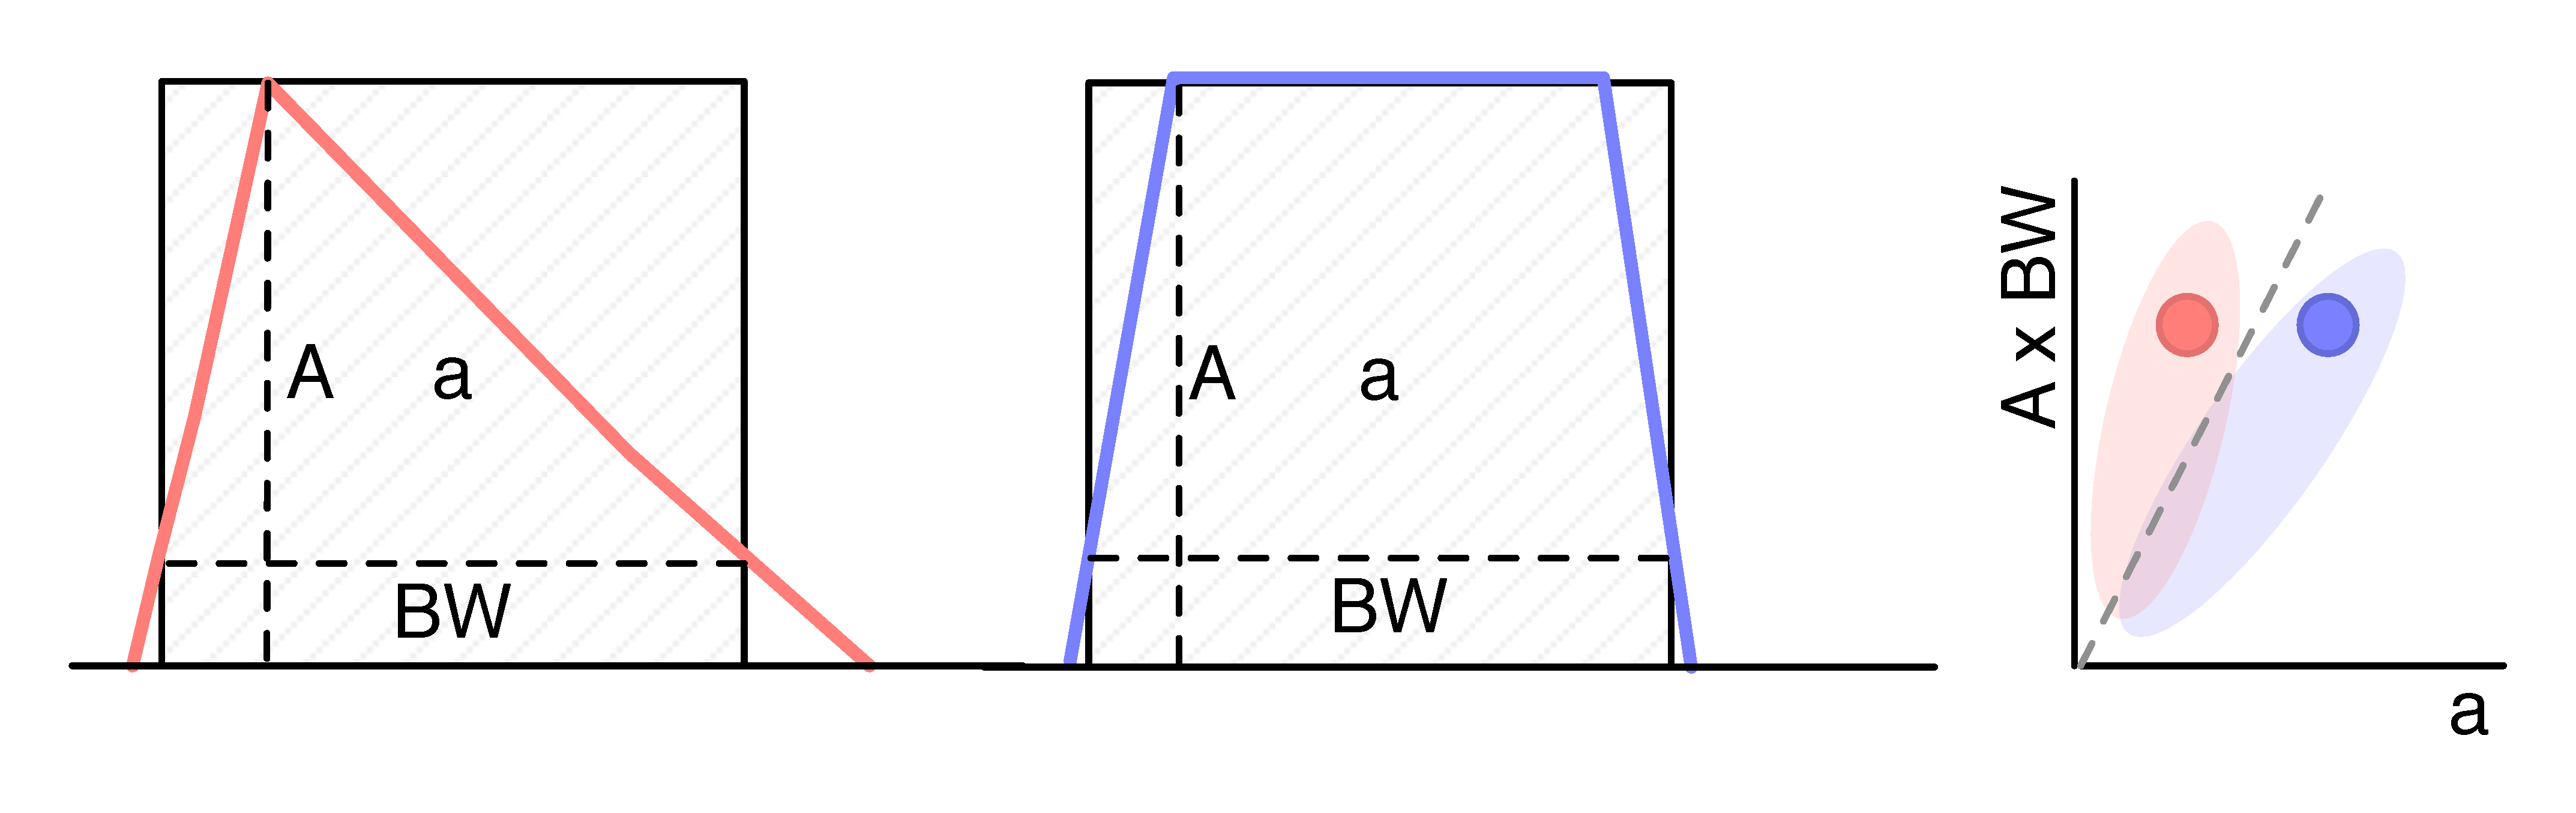
\includegraphics[width=0.7\textwidth]{05_current_monitoring/plots/formfac1}
\caption{Form Factor. The black squares show the calculated area of the pulse. The calculated area is similar to the measured area for rectangular pulses, but not so much for triangular pulses. The red and blue dot in the right plot are the value entries of the two pulses shown. The red and blue oval shapes depict the regions for the values expected for triangular and rectangular pulses. %By carefully choosing the linear qualifier (black line) and taking only the entries below the cut rectangular pulses can be identified.
}
\label{fig:formfac1}
\end{figure}

%Every parameter set is saved into a histogram after analysis.  The falling slope is not even a physical quantity, but as will be shown later, can improve the identification. 


%\subsection{Real-time pulse shape analysis algorithm}
%\clearpage
%\section{Applications}
%\label{sec:applications}
%
%The FPGA firmware is designed for systems instrumented with CIVIDEC amplifiers and CIVIDEC sCVD diamond detectors. Three applications are available: \emph{Spectroscopy}, \emph{Pulse Shape Analysis} and \emph{Counter}, each optimised for a specific task. Their capabilities are described below. The firmware runs in ROSY, a readout system produced by CIVIDEC.
%
%\begin{description}
%\item[Spectroscopy] is a tool for measuring energy spectra of radioactive sources. It is used in combination with the CIVIDEC Cx spectroscopic charge amplifier. The signal from the charge amplifier is analysed in real time. The FPGA measures the maximum amplitude of the signal. The amplitude value is ready at the end of the pulse and is stored in the amplitude histogram. Immediately after, the analysis is reset and the system is ready for a new acquisition. Upon request from the software, the histogram is read out, during which the analysis is paused. In addition to the histogram building, the firmware can also store raw pulse waveforms, which can be then read out by the software. The maximum allowed throughput is 10$^6$ counts per second.
%
%\item[Pulse Shape Analysis] is a tool for measuring energy spectra of radioactive sources, with an additional feature. It can identify the type of radiation detected by the diamond detector. By means of the pulse analysis it can subtract the background radiation and only measure the signals from the defined radiation source. It is used in combination with the CIVIDEC C2 broadband current amplifier. The firmware receives a current pulse from the detector and digitises it. The pulse is then analysed and parametrised. The analysis module measures its maximum amplitude, full width at half maximum (FWHM), baseline amplitude, falling slope and its area. Then it compares the obtained pulse parameters with the qualifiers set by the software and determines what type of radiation hit the diamond detector. Depending on the qualifiers, the pulse can either be \emph{accepted} or \emph{rejected}. The firmware then stores the parameters of the analysed pulse into histograms. Two histograms exist for each parameter: one for all pulses and one for accepted pulses. In addition, there is one 2D histogram (a scatter plot), which can plot two parameters one with respect to the other. Upon request from the software, all histograms are read out, during which the analysis is paused. The maximum allowed throughput is 1~million counts per second.
%
%\item[Counter] is a tool that measures the count rate and the mean time during counts. It is used in combination with the CIVIDEC Cx, C6 or C2 amplifier. It contains one histogram which holds the information about the mean time during counts. The counter is operational also during the readout of the histogram. The highest counting rate with enabled histogram writing is 3$\times10^7~s^{-1}$.
% 
%\end{description}



\section{Description of the firmware}
The application is built on top of the existing platform that handles the low-level connectivity with the hardware. It also provides the interface to the ADC data, the input/output registers and the USB data transfer. The PSA application has a set of modules that handle the data input and output and a module for signal analysis, as shown in figure~\ref{fig:application}. 
%The data handling modules are very similar in all the applications to ensure compatibility of the communication between software and firmware and the readout data format. 
The data handling layer consists of the final state machine (FSM), the histogram builder, the raw signal handler, the USB FIFO buffer and the register array.

The firmware is written entirely in VHDL. The diagram in figure~\ref{fig:application} shows the module architecture. The ADC provides the module with 32 digitised signal samples every clock cycle. The signal is routed directly to the pulse analyser and into the raw signal handler. The analyser outputs are connected to I/O registers and to histogram buffers. Both the histogram buffers and raw signal buffers are connected to the USB FIFO through a multiplexor. The firmware communication to the controller is done via input/output (I/O) registers (control and status registers, counters) and serially via USB (histogram data, waveforms). 


\begin{figure}[!t]
\centering
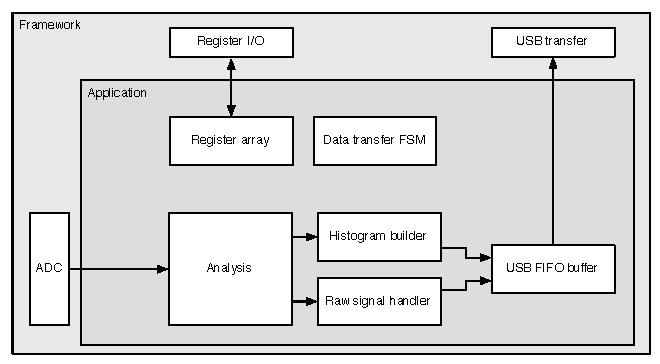
\includegraphics[width=0.7\textwidth]{05_current_monitoring/plots/application}
\caption{Firmware design structure.}
\label{fig:application}
\end{figure}


\subsection{Design constraints}
\begin{description}
\item[Speed] The ADC provides 32 8-bit samples on every 6.4~ns clock cycle. It is not possible to e.g. sum all 32 values in a single cycle, because the summation takes too long to complete. This is why the summation has to be pipelined and carried out in three cycles. This adds up to the analysis duration, which in turn decreases the maximum pulse rate.
\item[Firmware size] The PSA application makes use of a number of FIFO and RAM buffers to store the pulse waveforms and histograms. 48 32k block RAM modules have been used for the implementation, maxing out the available block RAM memory space on this FPGA. The analysis algorithm also takes up a significant portion of the FPGA fabric. Many of the operations are carried out on 256-bit long numbers received from the ADC, which quickly fills up the available logic. This is also why the place and route procedure takes a long time.
\item[Power consumption] The reduction of the power consumption is not crucial for the intended applications.
\end{description}


%=====================================================
\subsection{Analysis module}
\label{subsec:algorithm}
This module is different for different applications. The Pulse Shape Analysis (PSA) application has the most complex module design. The spectroscopy application only uses a small part of that design and the Counter application an even smaller one.


\begin{figure}[!t]
\centering
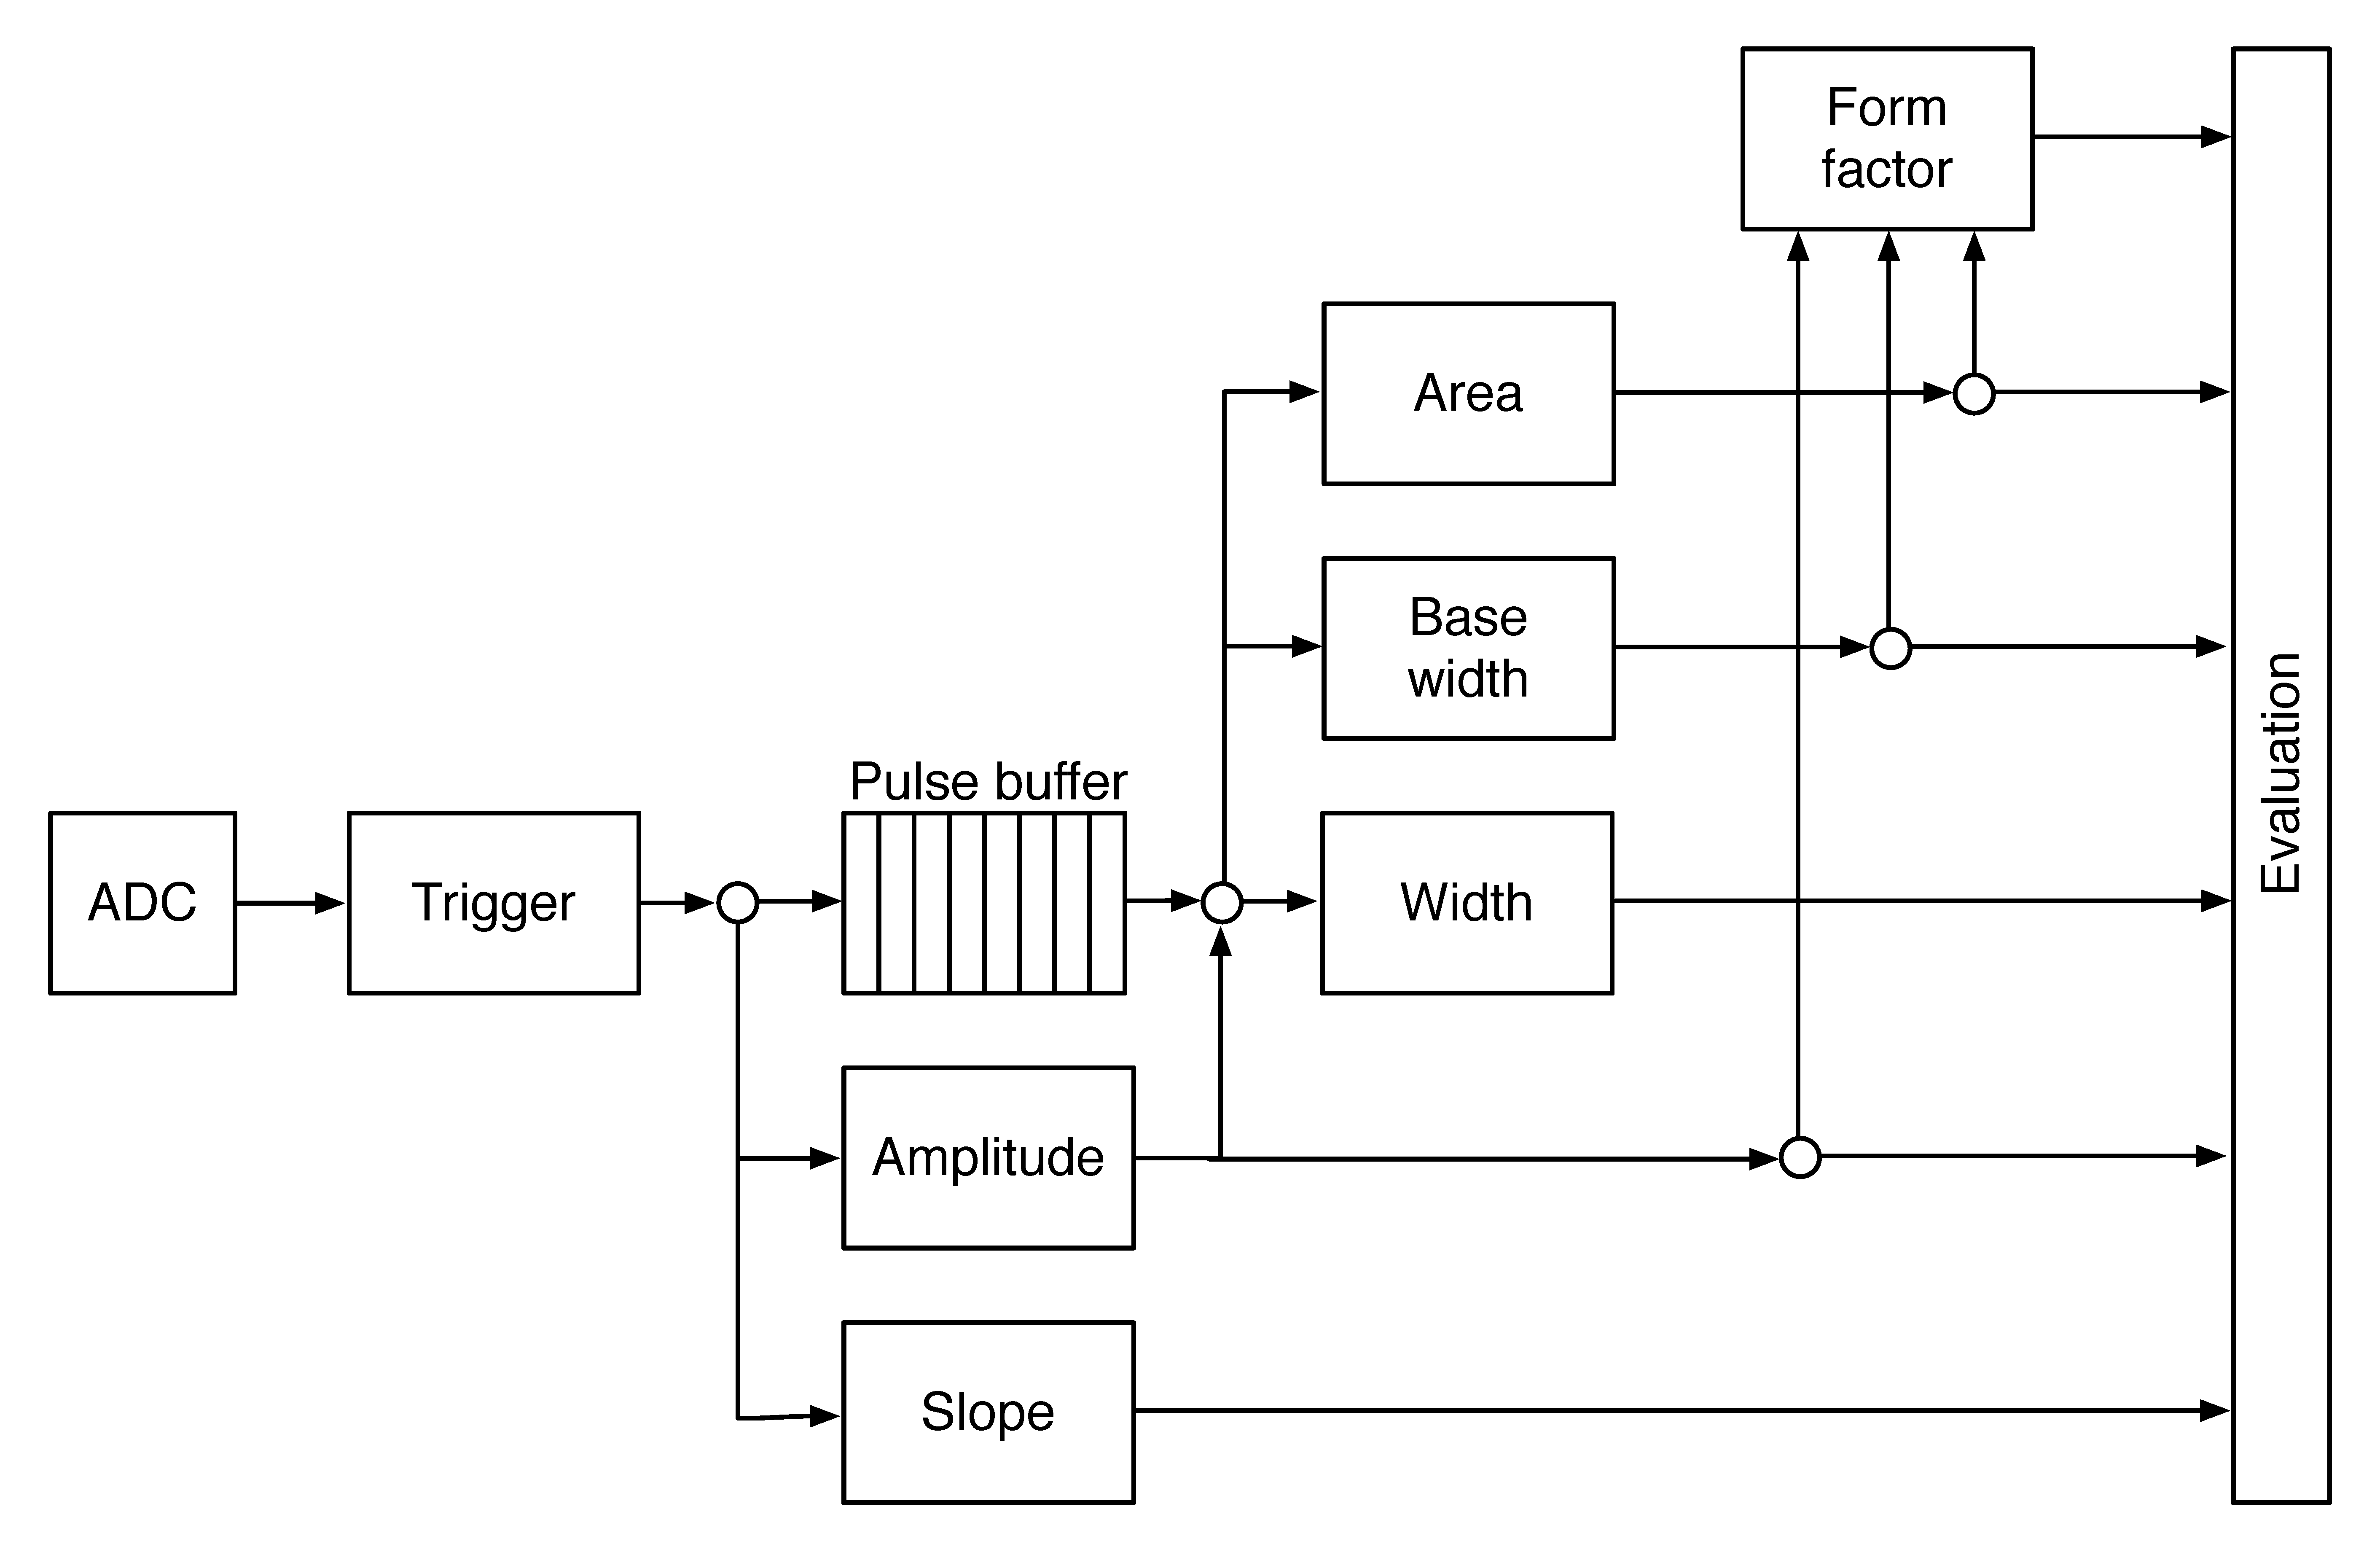
\includegraphics[width=0.7\textwidth]{05_current_monitoring/plots/analysis1}
\caption{Code design plan.}
\label{fig:architecture}
\end{figure}

The analysis (or parametrisation) is carried out in several steps, as shown in figure~\ref{fig:architecture}. The triggering block starts the readout upon signal threshold crossing. The maximum slope of the falling edge is observed. The Amplitude block calculates the pulse height and retains the maximum amplitude while pushing the signal into the pulse buffer. Then the entire pulse is clocked out of the buffer while its FWHM, baseline width and area are measured. Finally, the Form factor is calculated. At the end the Evaluation block takes in all the parametrised information and classifies the pulse according to user-defined cuts. 

%Figure~\ref{fig:pulseana} shows the timing of the data flow within the block. All submodules are described in detail in the following subsections. The waveform in figure~\ref{fig:waveform1} is a simplified representation of the pulse analysis process. The logic bits show which modules within the PSA are active at which stage of the analysis.
\begin{description}
\item[Triggering] module handles signal polarity swapping, triggering on threshold and defining the trigger window. The real-time processing algorithm allows for a positive or an inverted input signal. However, the PSA only handles positive-polarity pulses. Therefore a negative signal is swapped in the \textit{triggering} block. Signal analysis and readout are then triggered when the signal crosses a user-defined threshold. In addition, the signal has to be over the threshold for a defined number of samples. This is to avoid triggering on noise spikes.
A double clock cycle delay is used on the signal to make sure that the recorded signal window includes the rising edge of the pulse as well as some baseline before it. A \textit{trigger active} signal marks a window that contains the entire pulse including some baseline signal before and after it. 
The trigger can be vetoed by three signals: if the pulse analysis is still taking place, if the input signal exceeds the maximum voltage range or if the data transfer FSM is pausing the analysis due to data transfer to the controller.

%\subsubsection{Baseline producer}
%\label{subsub:base}
%This module has two functionalities. It carries out baseline noise filtering and it produces a baseline signal during a pulse. The filtering is implemented as a moving average of four data points. User can choose which four points to use: every first, second, third or fourth sample.
%
%Baseline signal during a pulse is used to calculate pulse height. It is produced by re-playing the last 64 data points of the baseline in a loop (an example shown in figure~\ref{fig:pulsepars}). It is implemented as a double register which replaces the real signal during the trigger window.


\item[Amplitude] block calculates the pulse height as a difference between the pulse and the baseline. It also finds the position of the maximum amplitude within the clock cycle. It receives 32 8-bit samples from the triggering block every clock cycle. Time delays in the logic prevent it to find the maximum value of the 32 samples within one clock cycle. Therefore the decision logic has been pipelined in three stages, which means that the final maximum value is ready three clock cycles after the end of the pulse.
\item[Pulse buffer] is a FIFO buffer that stores the signal while its amplitude is being measured. At the end of the pulse the FIFO is read out so that the remaining measurements can take place. 

\item[Width] block uses the maximum amplitude to determine the \emph{half-maximum} and to measure the FWHM. To do so, it counts the samples that are above the half-maximum amplitude. However, this method might also count high enough noise spikes before or after the pulse. Hence an improved method, which ``cleans'' the measurement of unintentional additional noise, has been implemented. It is described in section~\ref{sec:vecclean}.
\item[Baseline width] block is the same as the Width block, but it measures the width either at 50~\%, 25~\%, 12.5~\% or 6.25~\%, depending on the setting in the register. It also makes use of the special method described in~\ref{sec:vecclean} to avoid overestimations due to including noise in the measurement.
\item[Area] block measures the pulse area by summing up the amplitude values of the samples in the pulse. The boundaries of the summation are defined with the crossing of the amplitude above a certain threshold. Only the samples between those boundaries are summed up. The boundaries can be set at  50~\%, 25~\%, 12.5~\% or 6.25~\% of the maximum amplitude of the pulse. The area measurement makes use of the same routine as the FWHM and Baseline width block to remove the potential outlying samples.

\item[Falling slope] block measures the highest negative difference between amplitudes of two adjacent samples, thus getting the maximum negative slope of the pulse. It is an experimental routine, only used for academic purposes.
\item[Form factor] block is used as a special qualifier for particle identification. It compares the weighted measured area of the pulse with its weighted calculated ``form'', which is defined as the multiplication of the measured amplitude and baseline width. The equation is as follows:
\begin{equation}
\label{eq:formfactor1}
x\cdot a - y \cdot A \cdot BW \geq 0,
\end{equation}
where $a$ is the measured area, $A$ is the amplitude, $BW$ is the baseline width and $x$ and $y$ the user-defined weighting factors for the measured and calculated area. Typical values for these factors are 2 and 1, respectively. The output of the block is the boolean result of this equation.
\item[Evaluation] block takes in all the parameters from the analysis blocks and compares them against the user-defined qualifiers. If the parameters are within the bounds, the pulse is accepted, otherwise it is rejected. The corresponding counters within the block are incremented.

\end{description}


\subsection{Area and width measurement}
\label{sec:vecclean}
The routine for measuring pulse area and width must have a specific algorithm implemented to carry out the measurements correctly. The core point is that the routine precisely defines the edges of a pulse. It does so by means of \emph{vector cleaning}, presented in figure~\ref{fig:samplepulse}. An important input, beside the ADC data and the measurement threshold, is the position of the sample with the highest amplitude. 

The signal arrives from the ADC as a set of 32 8-bit samples every every clock cycle with a period of 6.4~ns. All 32 samples are compared against the width measurement threshold. If a sample value is equal or higher than this threshold, a binary 1 is set in a 32-bit \emph{vector} on the position corresponding to the position of the sample in the incoming ADC data set. The resulting vector might also include some noise at the edges of the pulse, depending on the height of the width measurement threshold. The old routine simply counts the binary ones in this vector to get the pulse width. This works well for measuring the FWHM because the threshold is high. However, for width measurements at 25~\%, 12.5~\% or 6.25~\% of the pulse height this might already become a problem, because the noise might be counted in as well. This is why the new routine cleans the outliers in this vector before counting the remaining ones in the clean vector. 

\begin{figure}[!t]
\centering
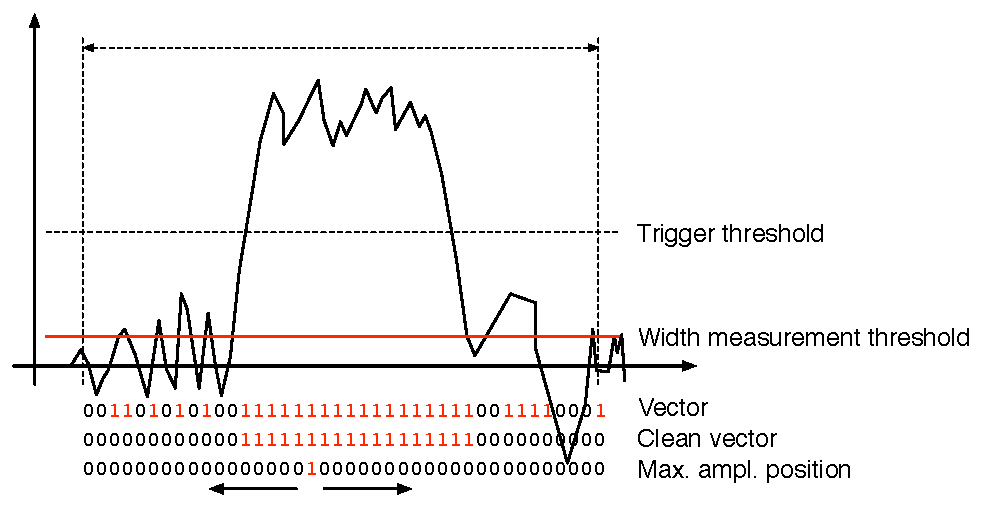
\includegraphics[width=0.7\textwidth]{05_current_monitoring/plots/pulse1}
\caption{A sample pulse. The first vector shows which samples are above the width measurement threshold. The second vector is a clean vector. The third line shows the position of the maximum amplitude. The vector cleaning algorithm starts from the maximum amplitude and continues in both ways along the vector. From the first falling edge on it sets all bits to 0.}
\label{fig:samplepulse}
\end{figure}

The routine starts from the position of the maximum height. It follows the vector in both ways and finds the first falling edge (0 at this position and 1 at the previous one). From there on it rewrites any binary 1 with a binary 0. The resulting clean vector only has one bunched set of binary ones which are summed, yielding a precise pulse width. The area measurement is similar - it only integrates over the samples marked in the clean vector. Both measurement routines, for area and for width, are implemented separately so that the area routine can have a different threshold set.

This section explains how the algorithm is designed. The idea for it was tested using Excel and was only afterwards ported to the VHDL. The underlying algorithm first cleans the vector. Then it passes the cleaned vector either to the width or area measurement, as shown in figures~\ref{fig:width} and \ref{fig:area}. The width measurement module only sums the ones in the vector whereas the area measurement module sums the data samples marked by the cleaned vector. Both modules issue a \emph{valid} signal when they finish the measurement.

\begin{figure}[!t]
\centering
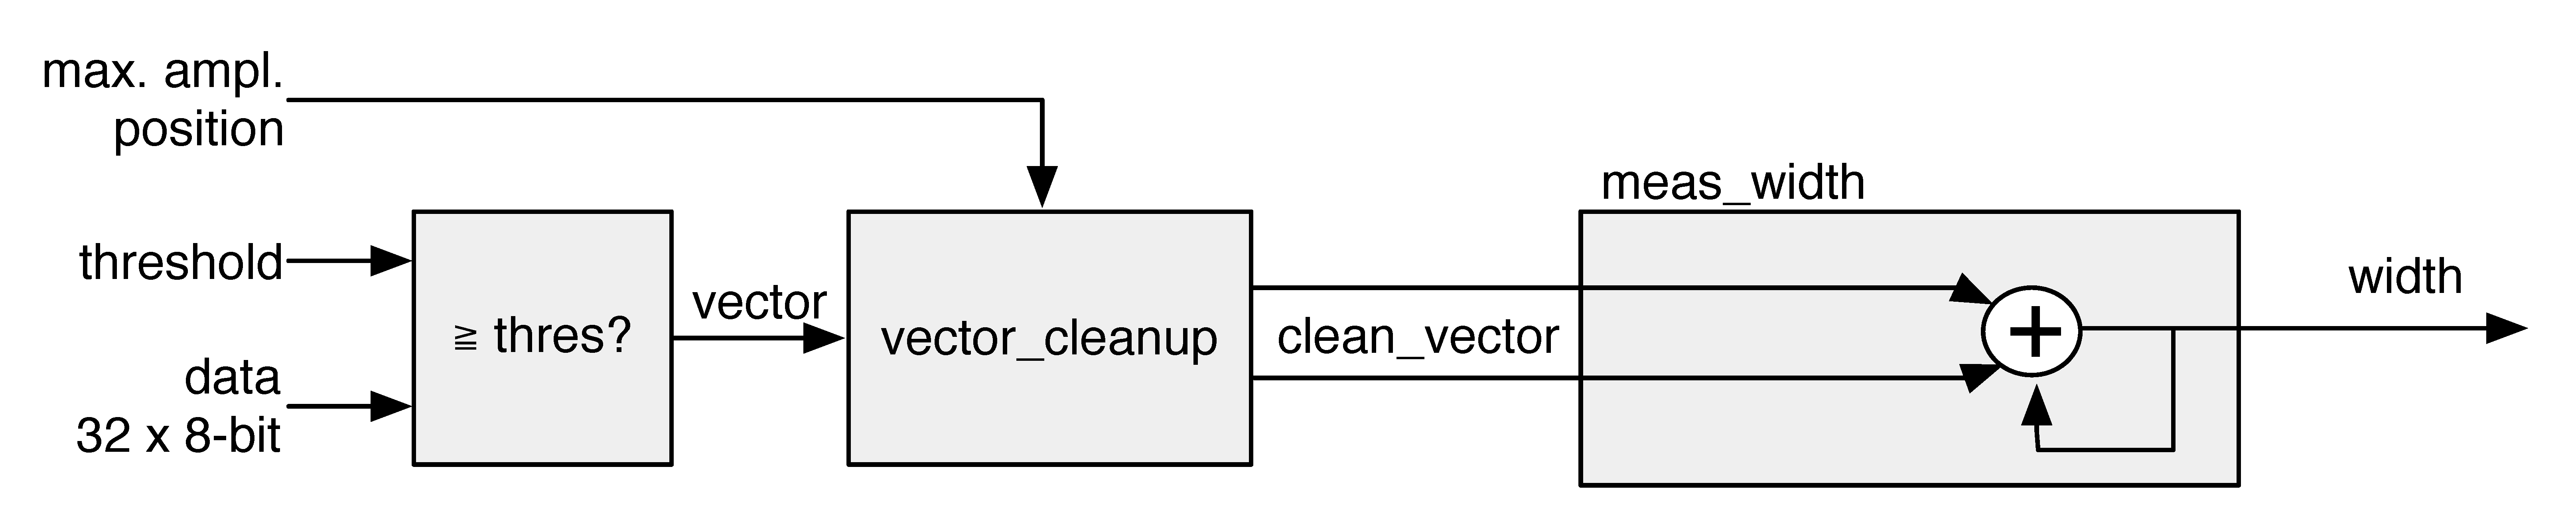
\includegraphics[width=0.95\textwidth]{05_current_monitoring/plots/width2}
\caption{This block counts the remaining binary ones in the clean vectors and outputs this value as the pulse width.}
\label{fig:width}
\end{figure}


\begin{figure}[!t]
\centering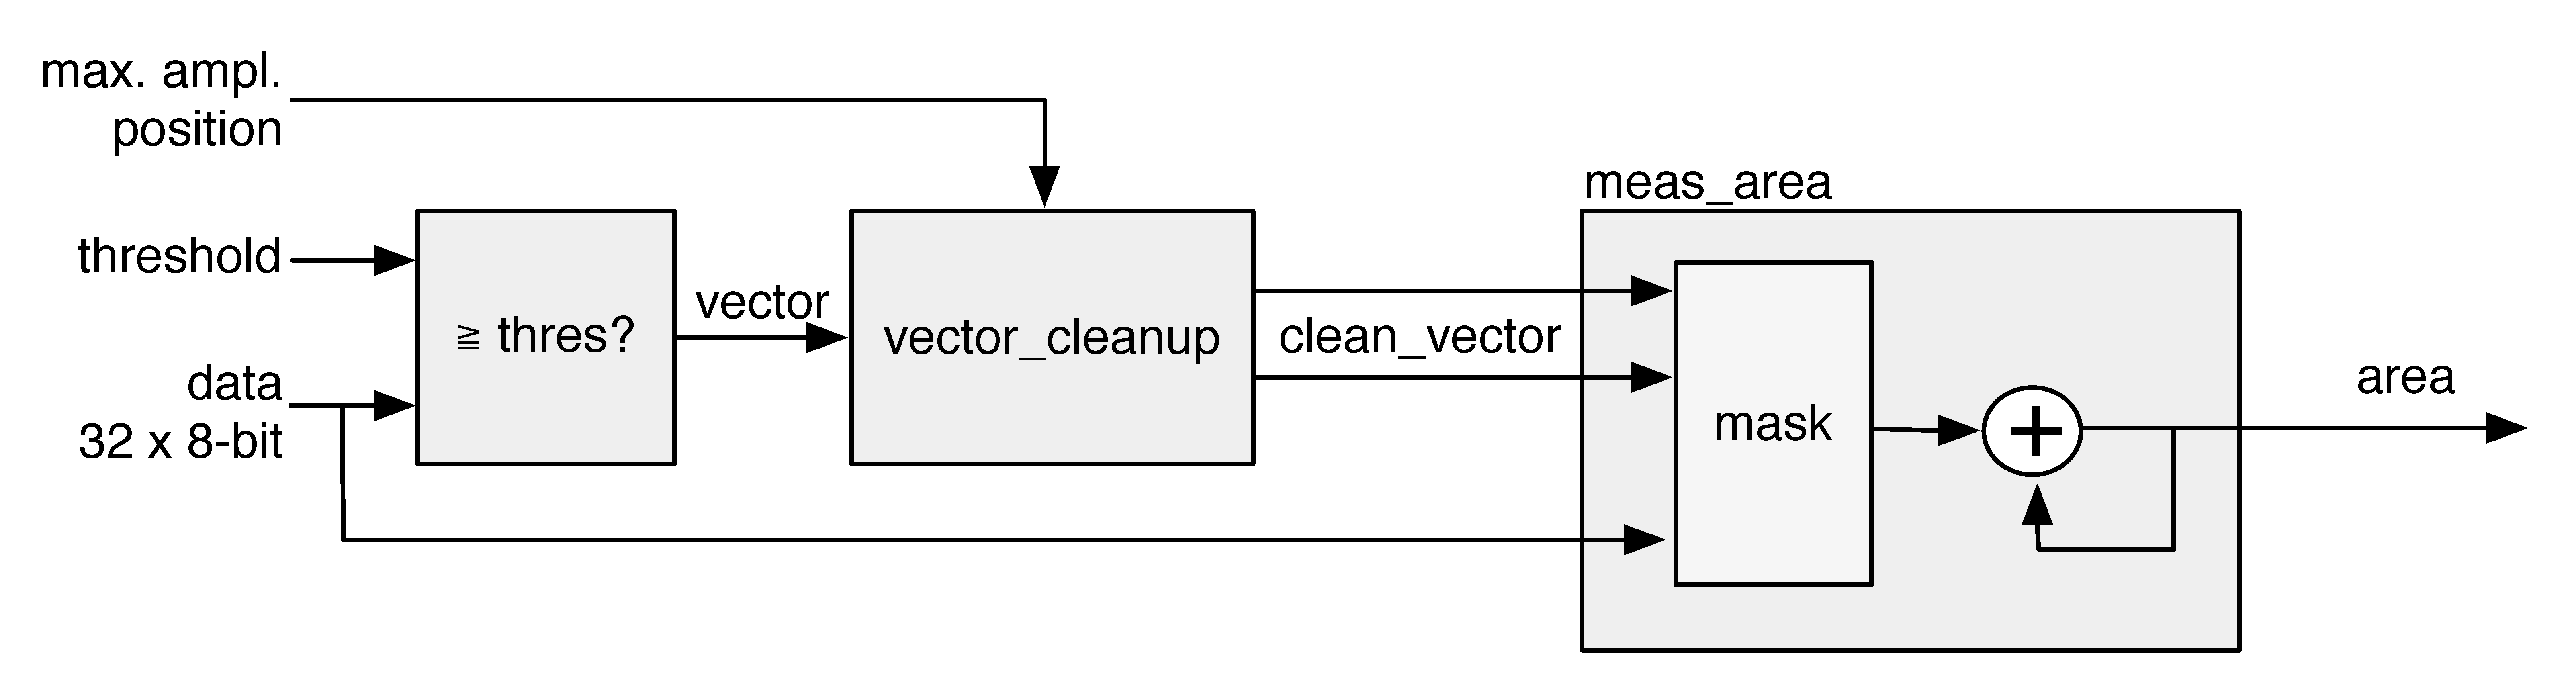
\includegraphics[width=0.95\textwidth]{05_current_monitoring/plots/area2}
\caption{This block masks the input data with the clean vector and sums the remaining samples.}
\label{fig:area}
\end{figure}


 
\subsubsection{Vector cleaning}
This is the most important block. Its inputs are: \emph{vector, parsing active, position of the max. amplitude (PA) and its delay (DA)}. PA is a 32-bit binary number that shows the position of the sample with the maximum amplitude within the data block (see figure~\ref{fig:samplepulse}) whereas the DA tells how many clock cycles after the start of the parsing this PA block is.
\begin{figure}[!t]
\centering
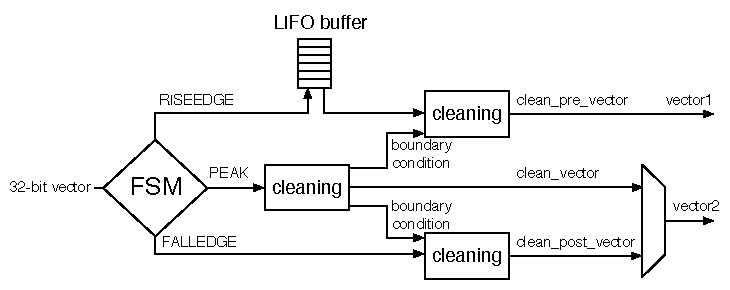
\includegraphics[width=0.9\textwidth]{05_current_monitoring/plots/vector_clean}
\caption{Vector cleaning routine outputs two vectors - one forward in time and one back in time starting from the peak of the pulse.}
\label{fig:routine}
\end{figure}
The vector cleaning module is designed as a final state machine (FSM) with the states IDLE, RISEEDGE, PEAK, FALLEDGE and READY.  The FSM is idle until it receives the \emph{active} signal from the external module, marking that the vector parsing has commenced. It switches to RISEEDGE, which starts two procedures: 1) it fills the vector of the pulse's rising edge into a last-in-first-out LIFO buffer (see figure~\ref{fig:routine}) and 2) counts down from the DA value. When this counter reaches 0, the FSM changes its state to PEAK because the current vector on the input is the one containing the maximum amplitude. This data block is sent through the \emph{peak algorithm}, which cleans the vector. The FSM switches to FALLEDGE state. Now both the previously buffered vector of the rising edge and current vector of the falling edge go through the \emph{pre- and post- algorithm} where they are cleaned, but they get their boundary conditions from the \emph{peak algorithm}. The output of this module is therefore two cleaned vectors in parallel -- one forward in time and the other backwards.



\subsubsection{Algorithm}
The underlying algorithm is sequential - it carries out a logic operation shown in figure~\ref{fig:log} on vector bit on position 0, uses the output of this operation for the operation on bit on position 1 and so on. This means that it has to carry out 32 logic operations per clock cycle. With each operation taking approximately 0.3~ns, the entire logic chain takes approximately 10~ns to complete. With only 6.4~ns per clock cycle, this means timing errors would occur. To fix the problem, a more complicated \emph{decimated algorithm} has been designed. It consists of two parallel logic chains. Each of the two only takes every second bit into account (Chain one: 0, 2, 4 ..., 30. Chain two: 1, 3, 5 ..., 31). This makes the chains effectively 16 bits long. The algorithm is run on the two chains and the results are merged together at the end as shown in figure~\ref{fig:algobase}. This effectively reduces the number of sequential logic operations to 18, which is within the timing constraints. 
%Nevertheless, to explain the algorithm, a non-decimated version will be shown first.
%This would need to be explained more in detail I guess...



\begin{figure}[!t]
\begin{tabular}{rr}
\subfloat{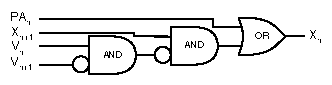
\includegraphics[width=0.47\textwidth]{05_current_monitoring/plots/logic1} \label{fig:logic1}} &
\subfloat{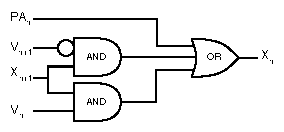
\includegraphics[width=0.47\textwidth]{05_current_monitoring/plots/logic2}  \label{fig:logic2}}
\end{tabular}
\caption{One logic step in the algorithm chain before and after Karnaugh minimisation.}
\label{fig:log}
\end{figure}

\begin{figure}[!t]
\centering
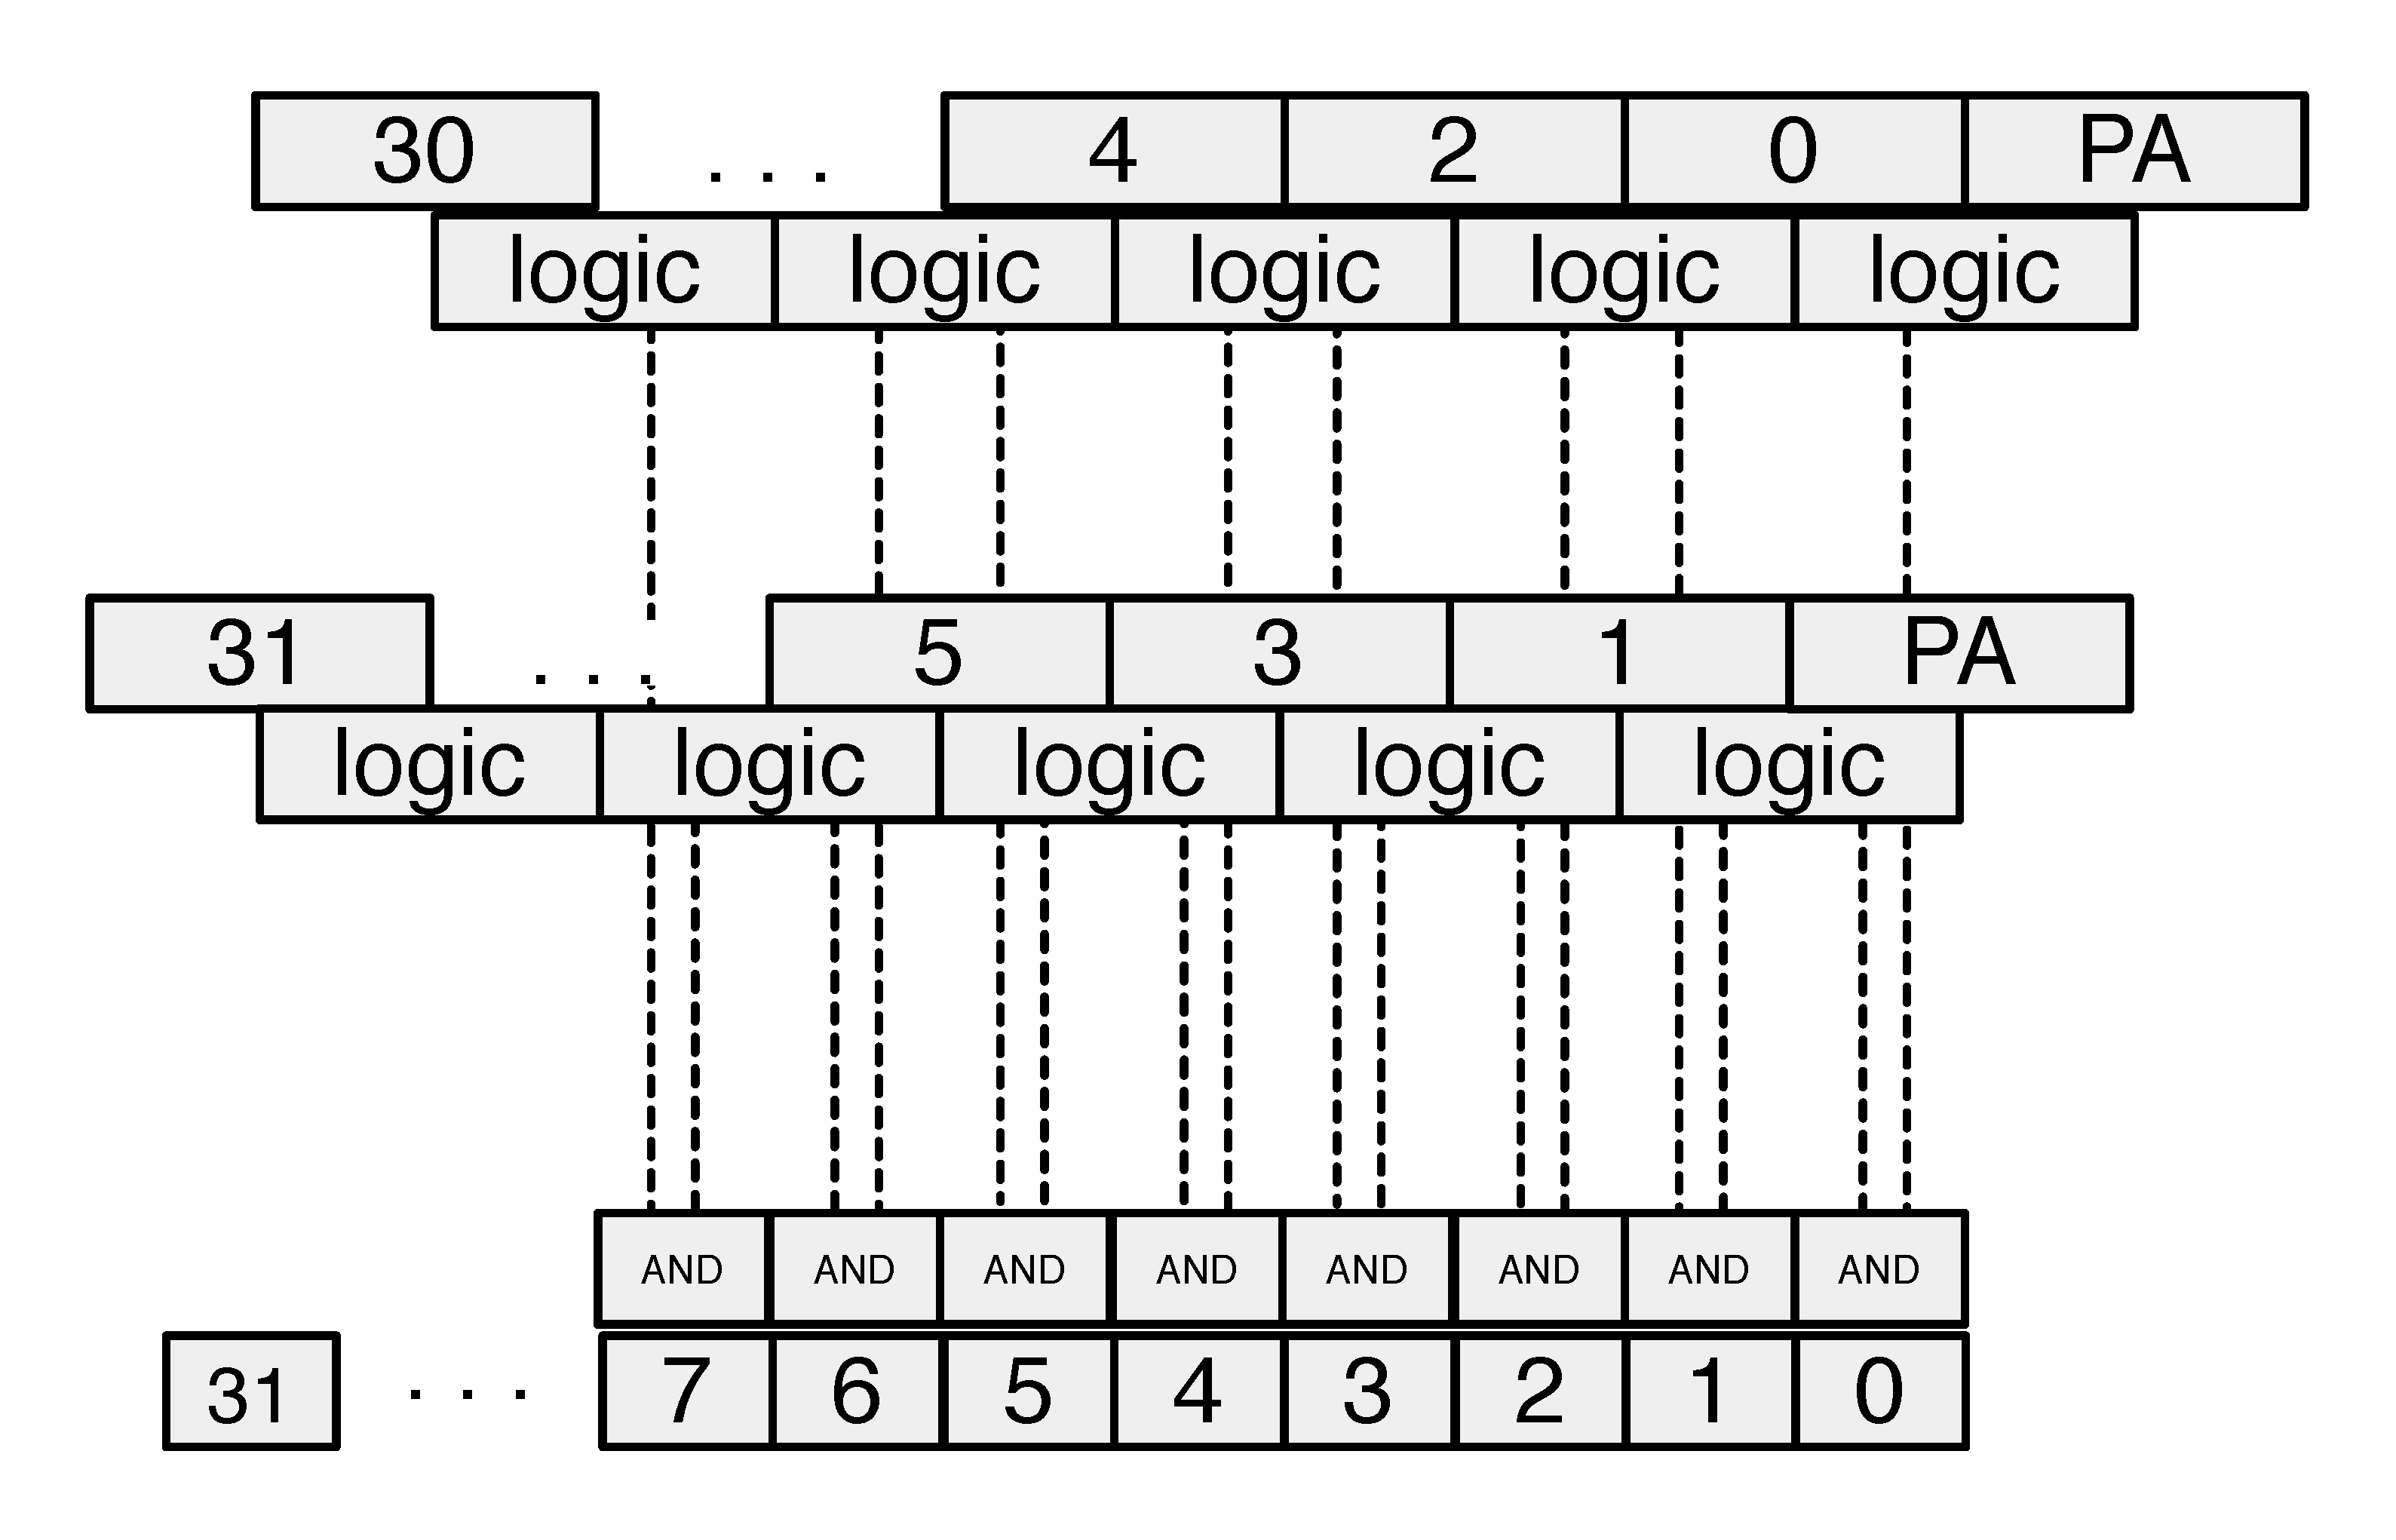
\includegraphics[width=0.5\textwidth]{05_current_monitoring/plots/algobase}
\caption{The vector is divided into two 16-bit logic chains. The algorithm logic is then run on the two chains separately. The results are then merged into one 32-bit clean vector by using a set of AND gates.}
\label{fig:algobase}
\end{figure}


\section{Control and data interface}
Communication between the device and the controller PC is done via the API functions provided by the producer. In addition, the API used by CIVIDEC has access to several extra functions. These allow the user to download a customised bitfile to the FPGA, access the I/O registers and use the USB data transfer.

\subsection{Software}
The software has been designed in C++ in several levels of abstraction. Figure~\ref{fig:controller} shows the structure of the classes. The classes Device, PSA and RawSignalHandler are there to make it easier to read and understand the controller code. In principle the PSfunctions can also be accessed directly by the controller, but for this the instruction sequences must be well known and understood. 

\begin{figure}[!t]
\centering
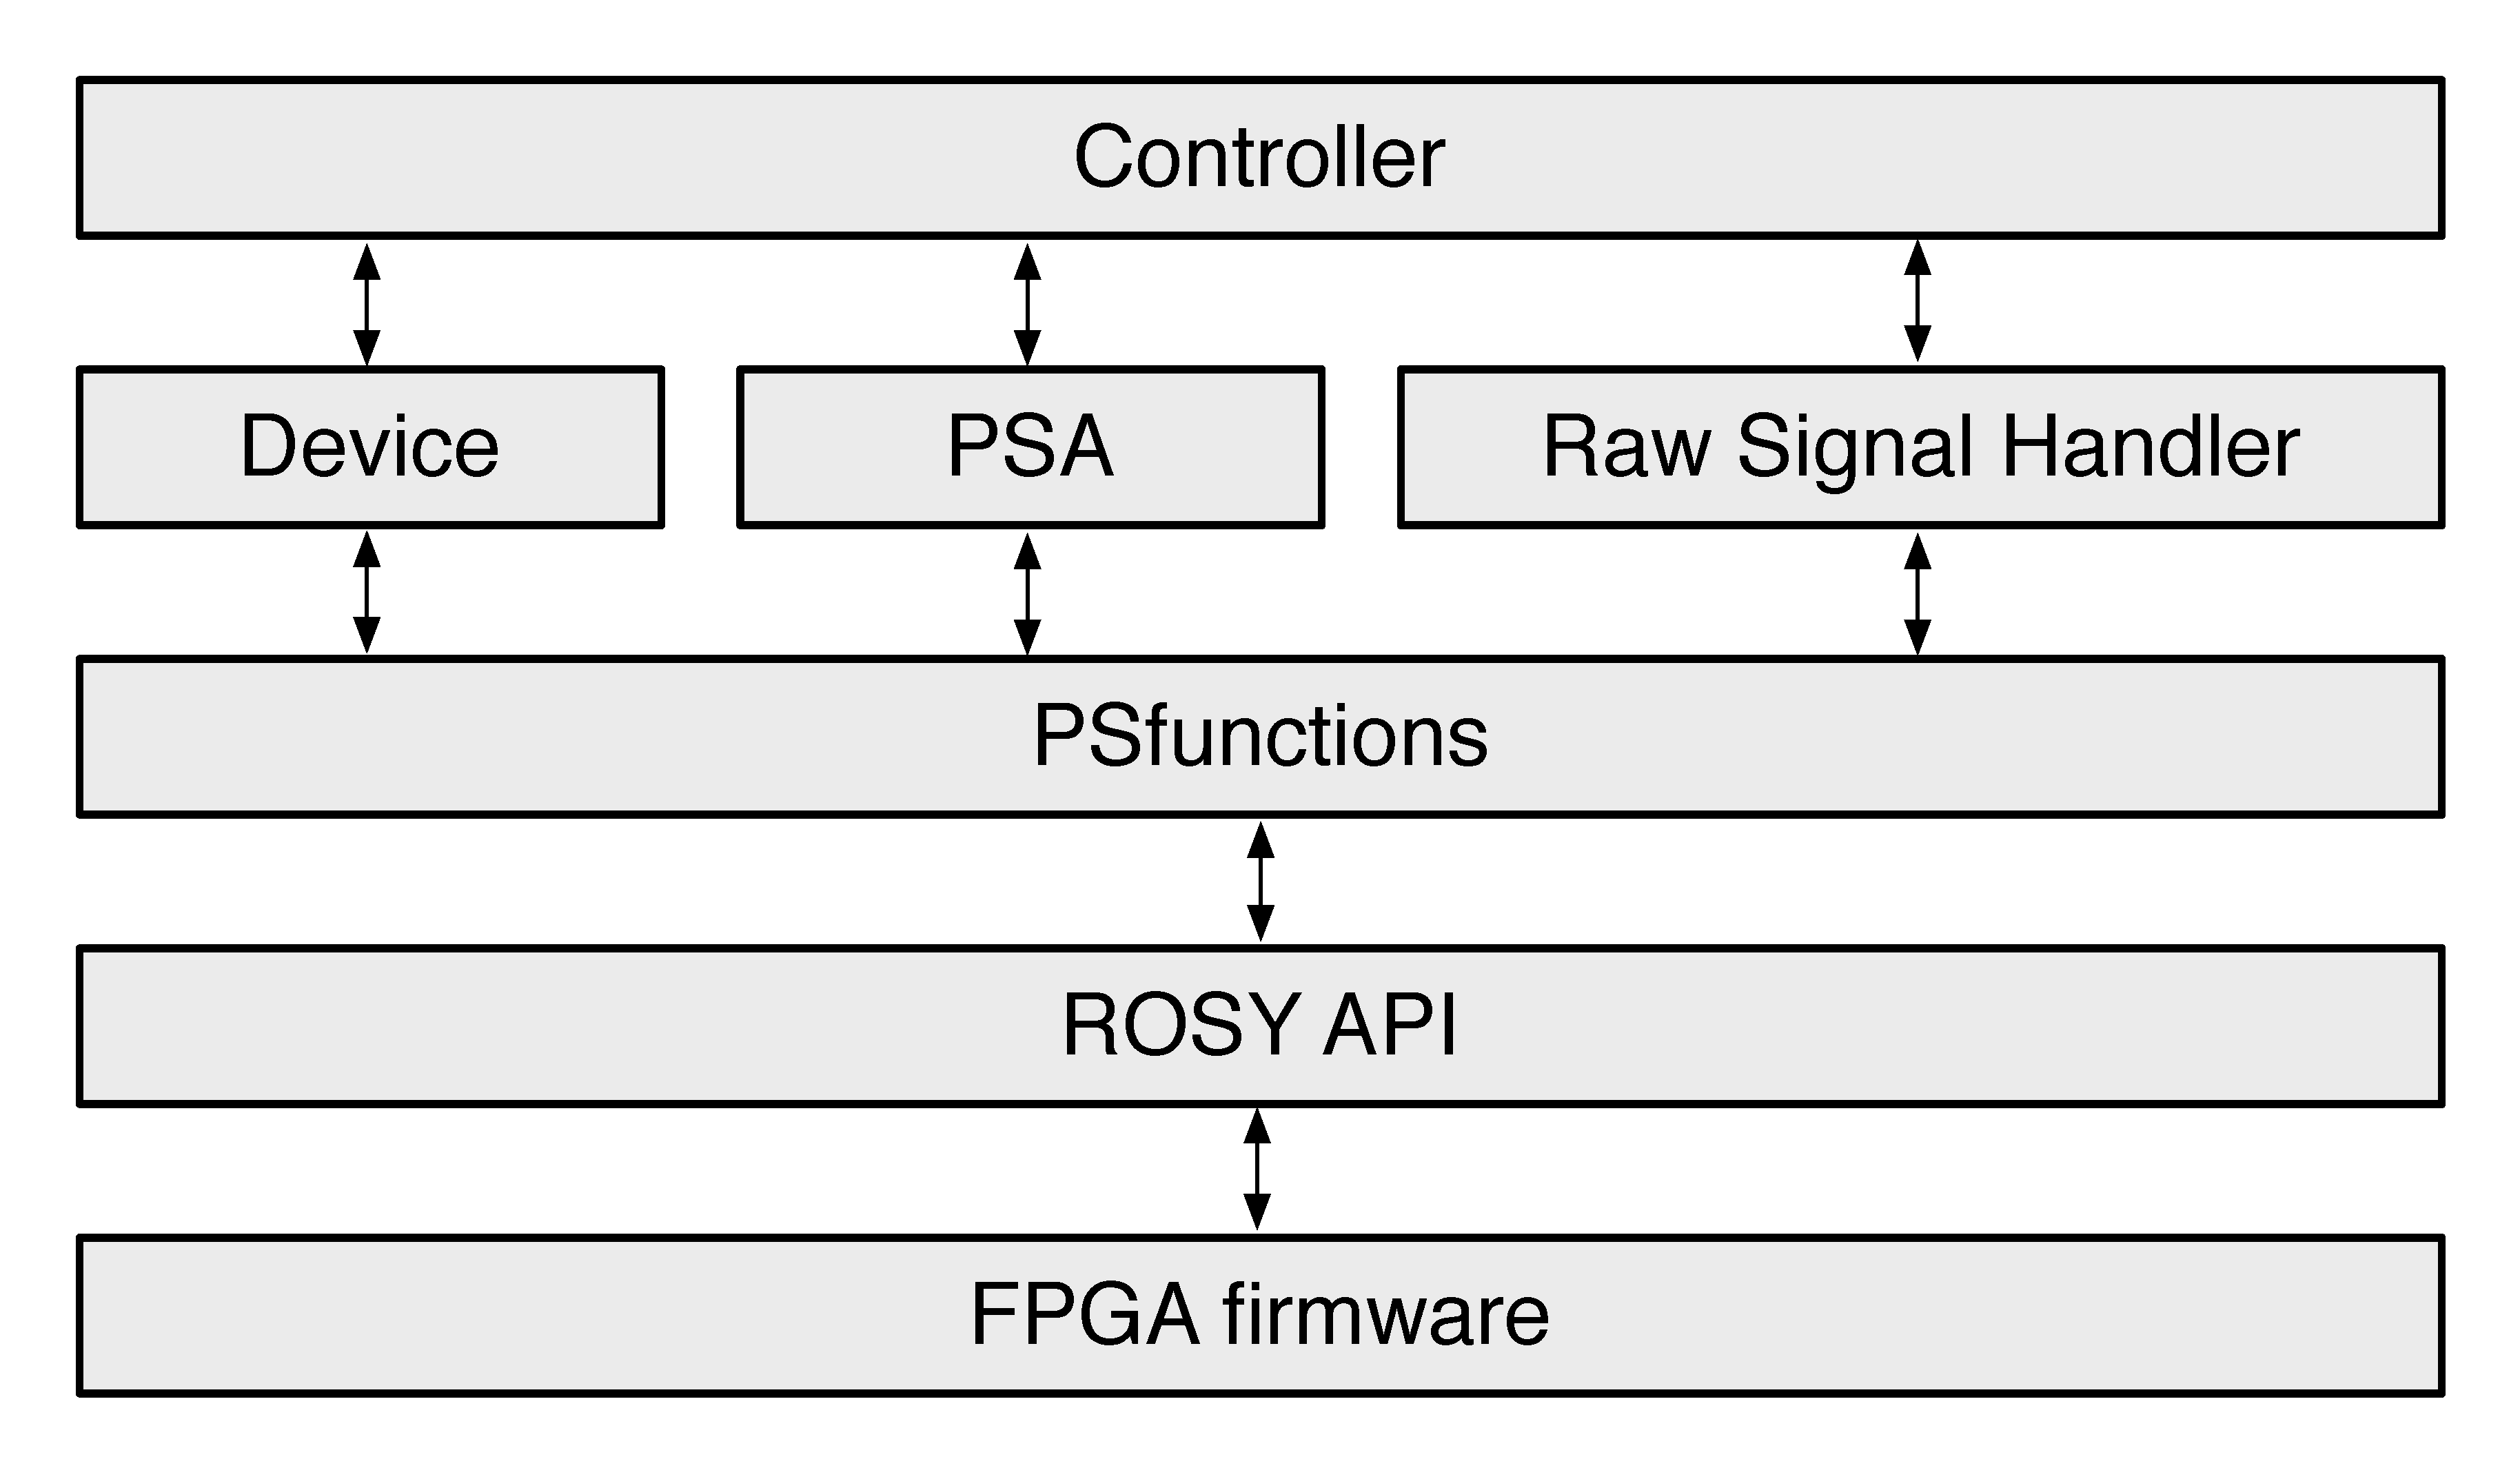
\includegraphics[width=0.45\textwidth]{05_current_monitoring/plots/controller}
\caption{Abstraction levels of the controller software.}
\label{fig:controller}
\end{figure}

\subsection{Data readout}
The device records the data in two forms - as signal waveforms and as histograms of analysed pulse parameters. Both are available upon request from the controller. Only one of the two can be transferred via the USB line at a time. 
%The waveforms are read out as a series of 64 pulses whereas the histograms are 

The waveforms are saved into a FIFO buffer, which can hold up to 64 pulses of the length of $\sim$500~samples. The data format for each pulse is such that it starts with a header containing the pulse timestamp and the sequential number, continues with the data samples and ends with a header containing all the measured parameters (width, amplitude, area, fallling slope and form factor). When the FIFO is full, it issues a flag, which tells the controller that the data buffer is ready for readout. 

The histograms are implemented into the FPGA's Block RAM. Their sizes range from 256 to 4'096 bins (8-bit to 12-bit histograms, respectively), depending on the required histogram resolution. For instance, the width parameter is measured with a 0.2~ns resolution and the expected maximum pulse width is less than 20~ns. This yields the maximum range of 100 bins, making an 8-bit histogram sufficiently large. The amplitude histogram range is defined by the 8-bit resolution of the ADC. The area measurement, however, yields higher values and can therefore have a more refined 12-bit binning. Finally, a single 12-bit 2D histogram is included, with six bits for every axis. It is used as an online scatter plot for comparing two measured parameters. An example for it is a comparison of the width against the area, which can help the user determine the cuts that need to be applied to the measurement. All implemented 2-D plots are shown in section~\ref{sec:sourcecalib}.




























% ---------------------------------------------------------------------------------------------------------------
%\clearpage
\section{Performance results}
\label{sec:perres}
% ---------------------------------------------------------------------------------------------------------------
The PSA was tested in the laboratory first using a pulse generator and then with a radioactive sources. This section contains the results of the performance tests.

\subsection{Tests with a pulse generator}
\subsubsection{Trigger rate}
A pulse generator was used to verify the highest achievable rate at which the PSA still analyses every incoming pulse. The final state machine implemented in the pulse analysis module prevents the triggering block from issuing a trigger due to an incoming pulse if the previous analysis is still ongoing. Given that all the pulses have the same length, the analysis duration must always be the same. When the time between the incoming pulses is shorter than the time of the analysis, the pulses are not analysed. Figure~\ref{fig:trigrate} shows the sharp decline in the percentage of the analysed pulses when reaching the rate of 6~MHz. Therefore the overall analysis duration for a 10~ns pulse is approximately 200~ns.

\begin{figure}[!t]
\centering
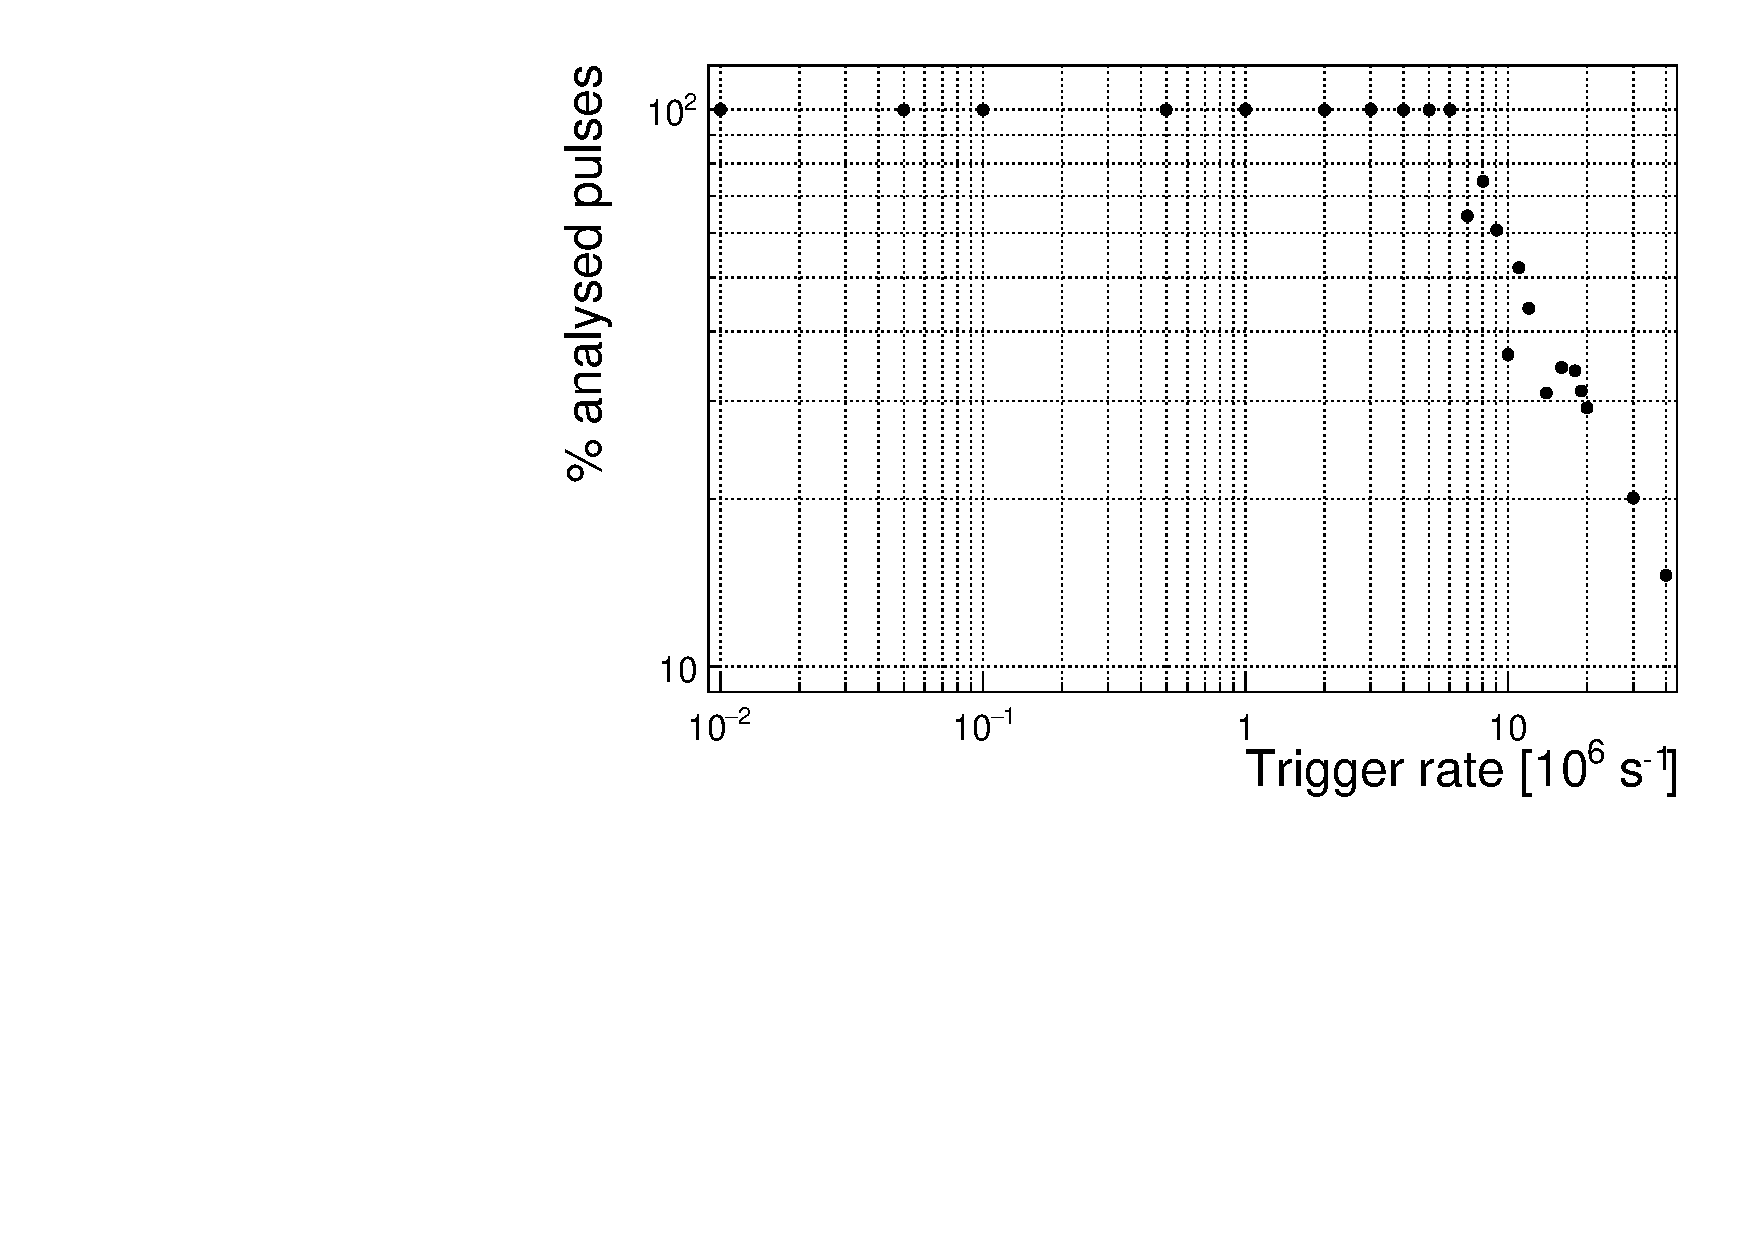
\includegraphics[width=0.7\textwidth]{../scripts/05_current_monitoring/PulseGenTests/plots/freq}
\caption{This figure shows the capability of the device to analyse all arriving pulses for a range of input frequencies. The highest achievable rate with zero lost pulses is $6\times10^6$~s$^{-1}$.}
\label{fig:trigrate}
\end{figure}

\subsubsection{Linearity}
A pulse generator was used to verify the linearity of the measurements across all input ranges. The pulse width and the amplitude were varied and measured both with the oscilloscope and the PSA to estimate the systematic error of the PSA measurements with respect to those taken by the oscilloscope. The results are shown in figures~\ref{fig:ratioAmpl1} and~\ref{fig:ratioWidth1}. The measured amplitude error $e_\mathrm{ampl}$ is within $\pm$3~\% of the real value throughout the amplitude range. The width error $e_\mathrm{width}$, however, increases significantly in the lower width range. This stems from the low bandwidth limit of the PSA, which affects the pulse shape via a slow rising and falling time, effectively smearing the pulse along the time axis. Therefore the PSA cannot measure rectangular pulses shorter than 2~ns.

\begin{figure}[!t]
%\centering
\begin{tabular}{rrr}
\subfloat{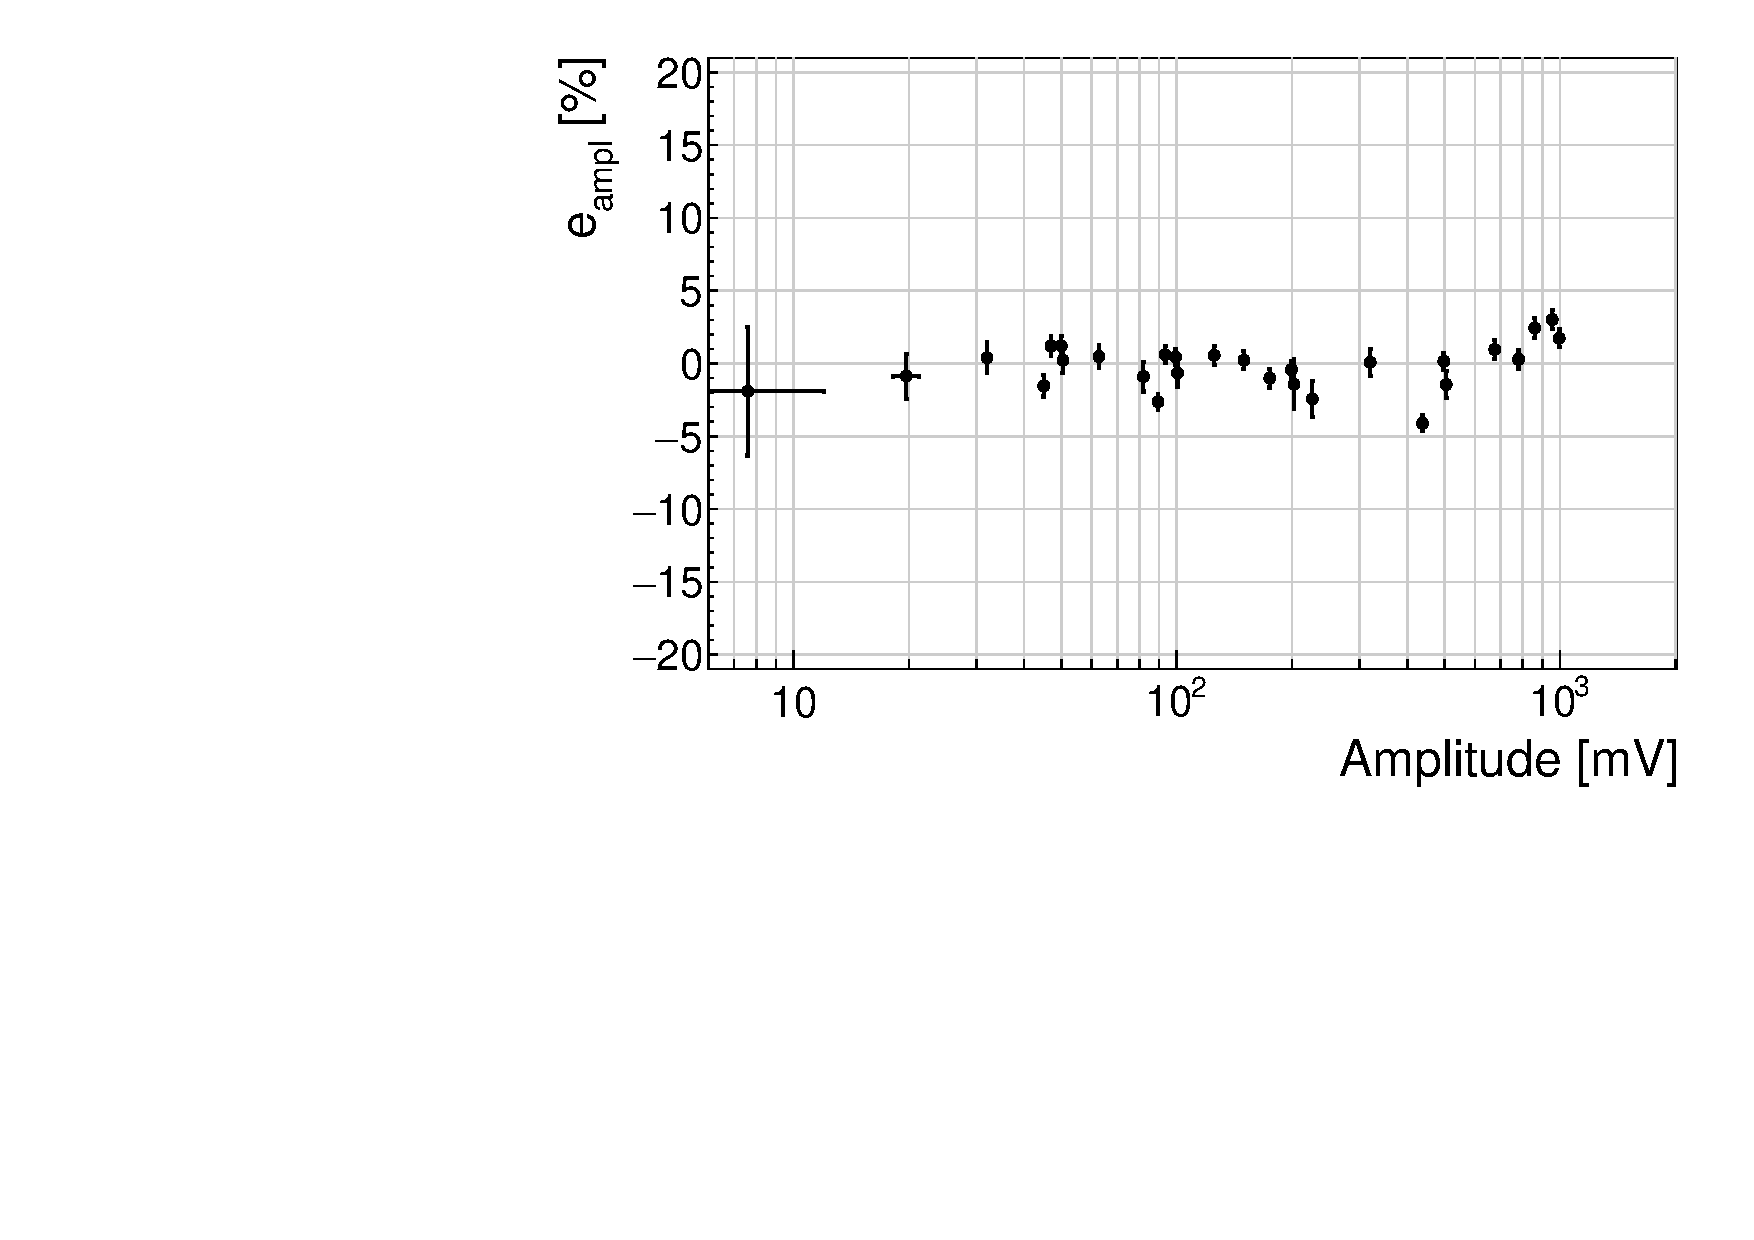
\includegraphics[width=0.47\textwidth]{../scripts/05_current_monitoring/PulseGenTests/plots/ratioAmpl1} \label{fig:ratioAmpl1}} &
\subfloat{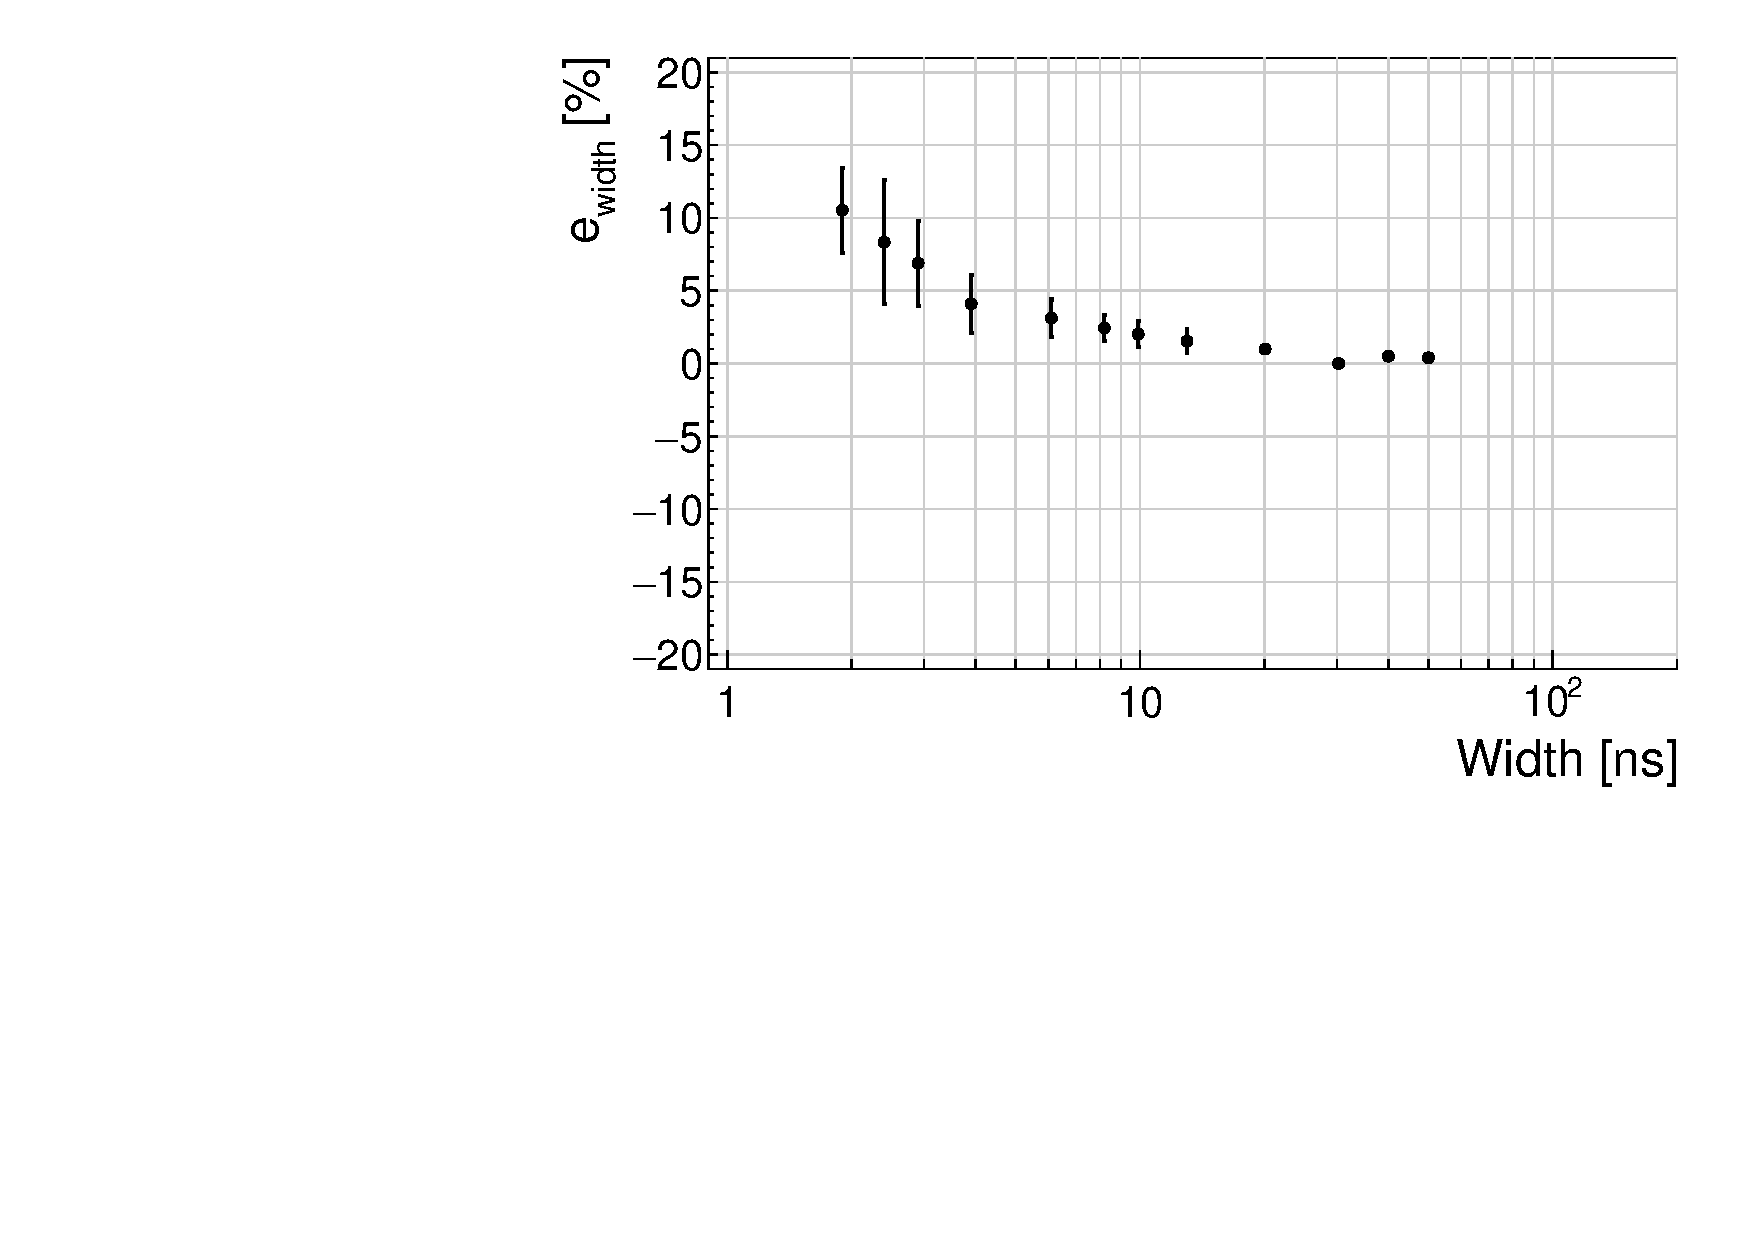
\includegraphics[width=0.47\textwidth]{../scripts/05_current_monitoring/PulseGenTests/plots/ratioWidth1}  \label{fig:ratioWidth1}}
\end{tabular}
\caption{These figures show the measurement errors for amplitude (left) and width (right) across the measurement range.}
\label{fig:ratiorange}
\end{figure}


\subsubsection{Stability}
The input pulse signal was superimposed with the white noise generated by a CIVIDEC noise generator with a variable attenuation. The mixed signal yielded pulses with an SNR ranging from 5 (very noisy) to 100 (noise negligible). The PSA then performed the pulse parametrisation at different SNRs without changing the pulse shape. The results of the measurement errors for amplitude, width and area are shown in figures~\ref{fig:snrAmpl1}, \ref{fig:snrWidth1} and \ref{fig:snrArea1}. The amplitude is highly overestimated at a low SNR (high noise). This is because the algorithm takes the peak of the signal as the maximum amplitude and these peaks are higher with a higher noise. Therefore the $e_\mathrm{ampl}$ is always positive and increasing with increasing noise. The width measurement, on the other hand, is stable even for the low SNR. The $e_\mathrm{width}$ does not exceed $\pm$5~\%. Finally, the mean of the area measurement error $e_\mathrm{area}$ is always 0, but the spread of the error increases with noise. This means that the increased noise only affects the resolution of the measured area spectrum, not its position.

\begin{figure}[!t]
%\centering
\begin{tabular}{rrr}
\subfloat{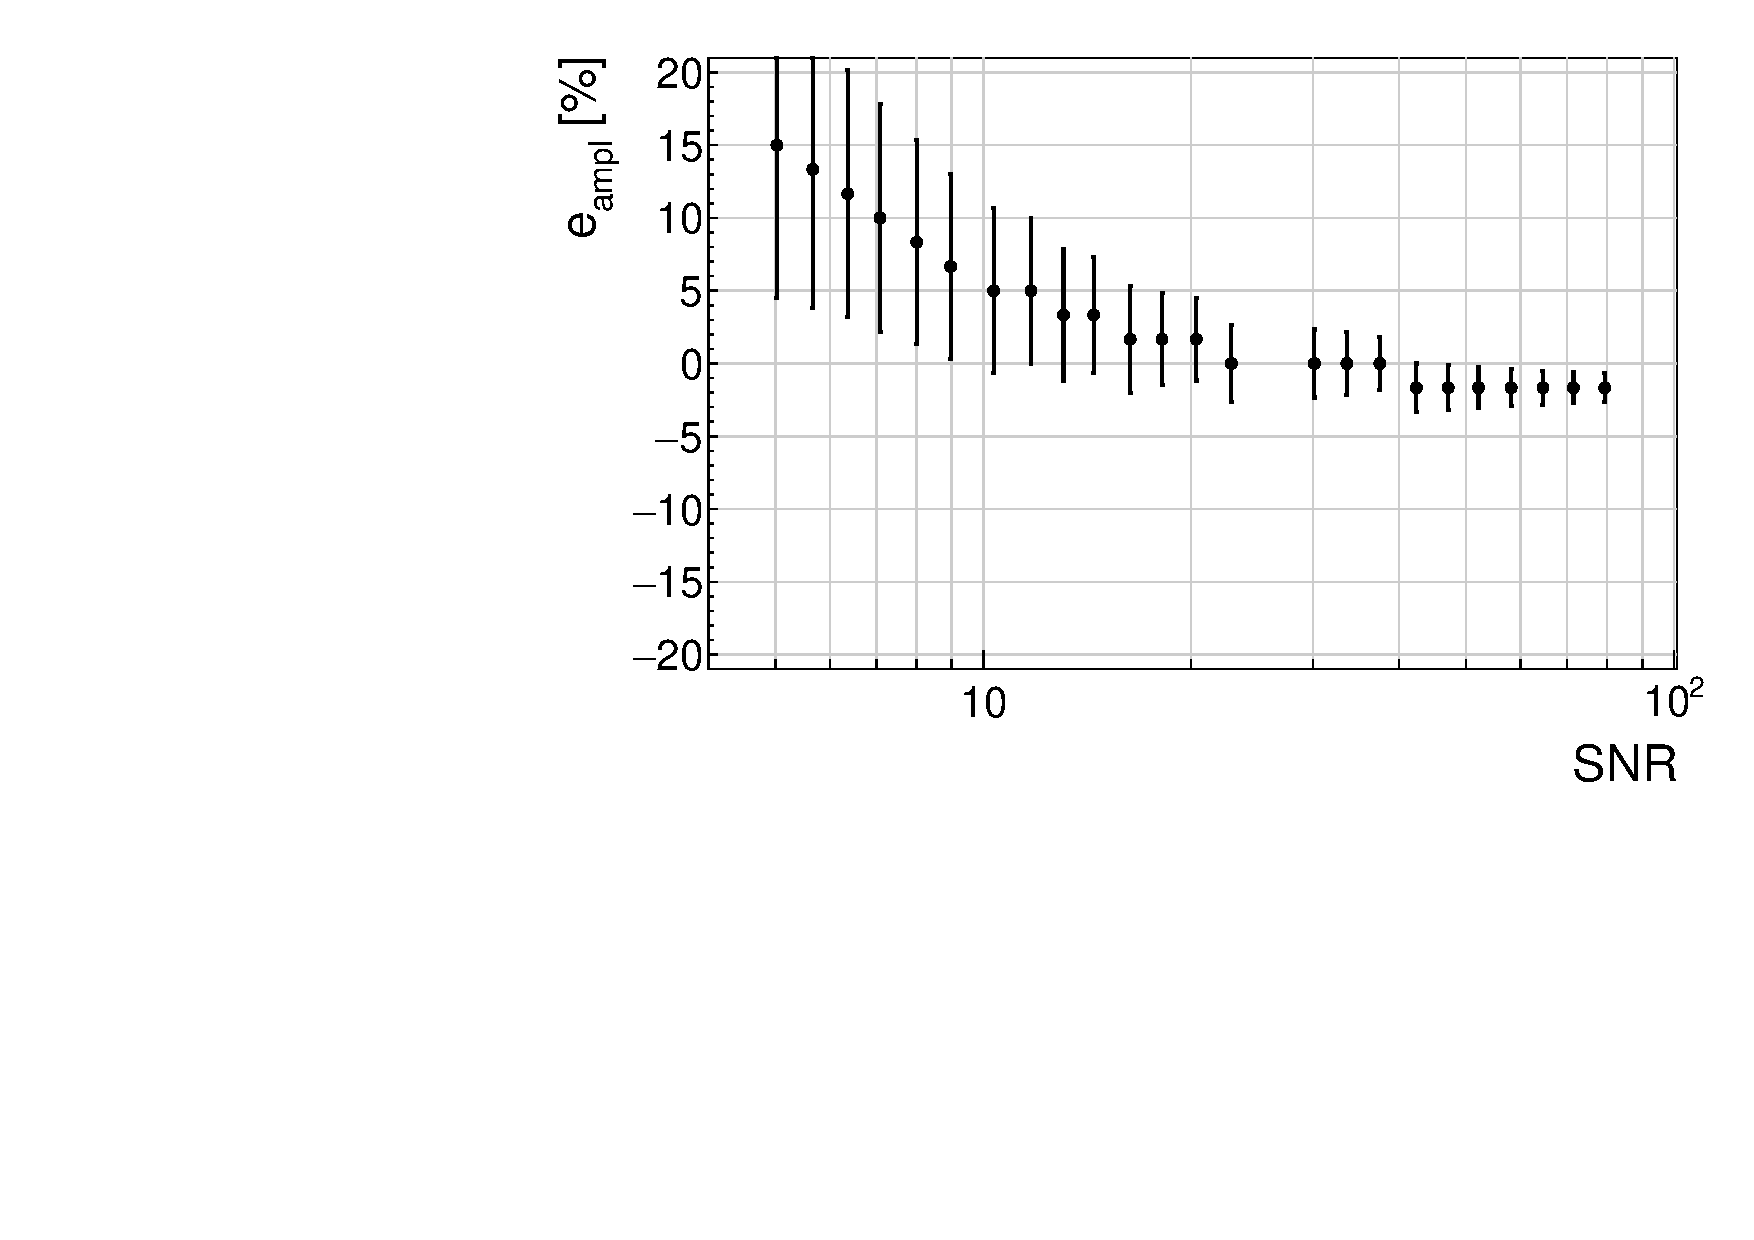
\includegraphics[width=0.47\textwidth]{../scripts/05_current_monitoring/PulseGenTests/plots/snrAmpl1} \label{fig:snrAmpl1}} &

\subfloat{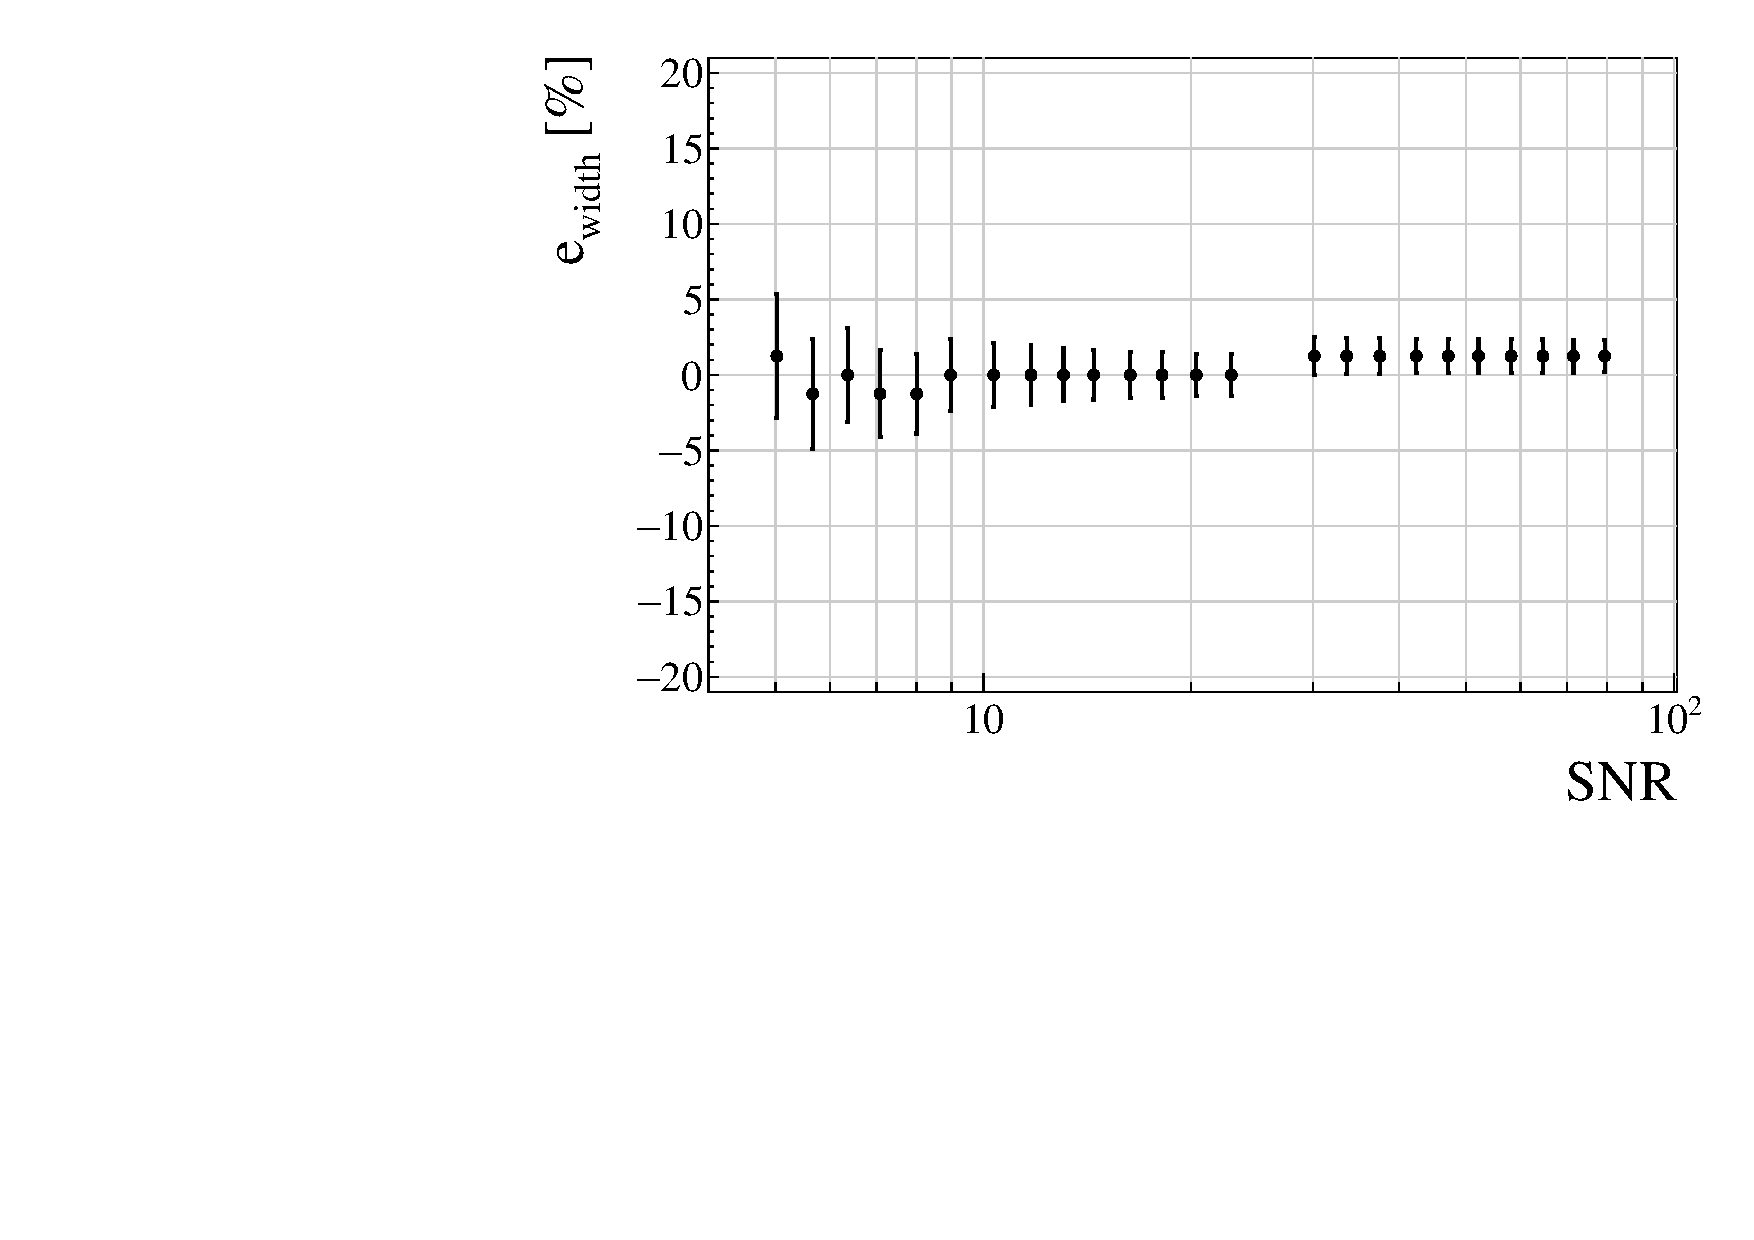
\includegraphics[width=0.47\textwidth]{../scripts/05_current_monitoring/PulseGenTests/plots/snrWidth1}  \label{fig:snrWidth1}} \\
 
%\subfloat[Linearity across the area range]{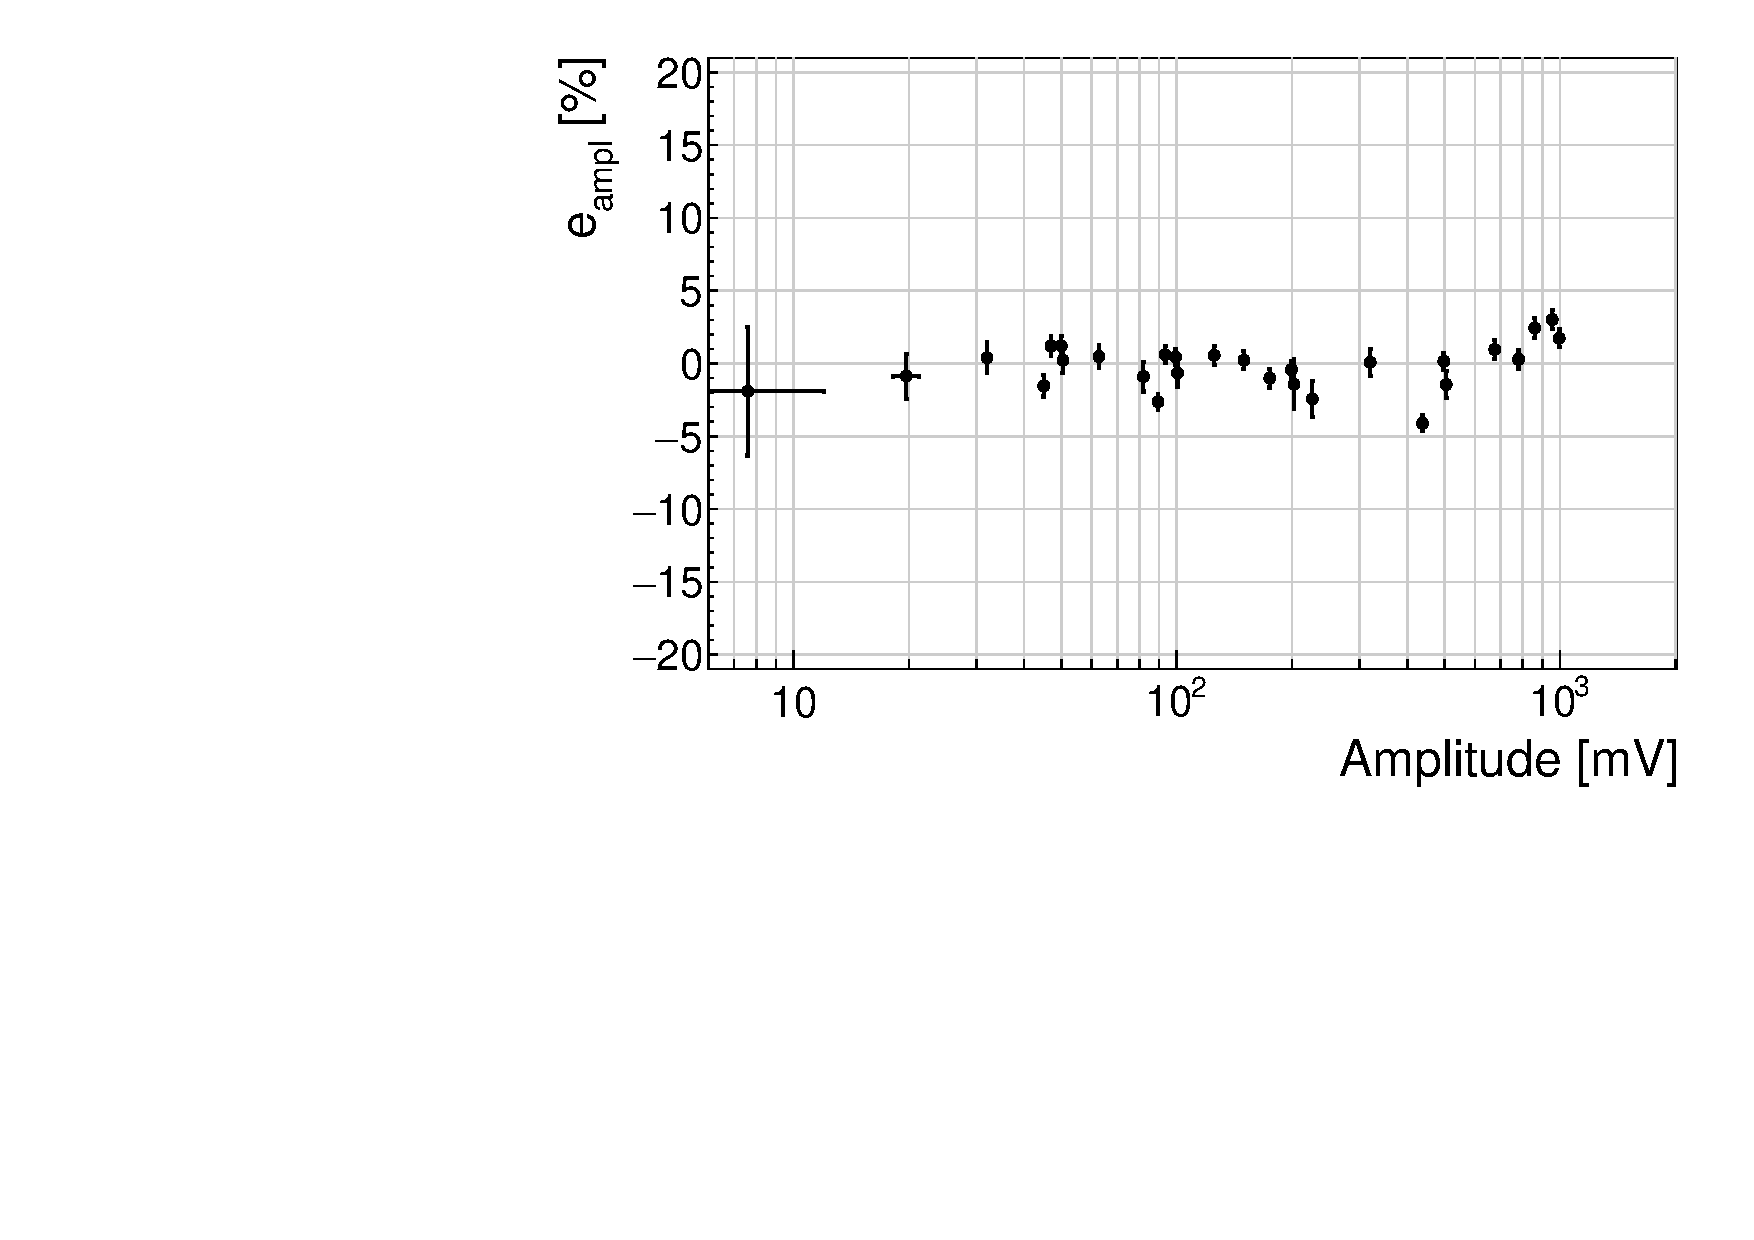
\includegraphics[width=0.45\textwidth]{../scripts/05_current_monitoring/PulseGenTests/plots/ratioAmpl1}  \label{fig:ratioArea1}} \\
\subfloat{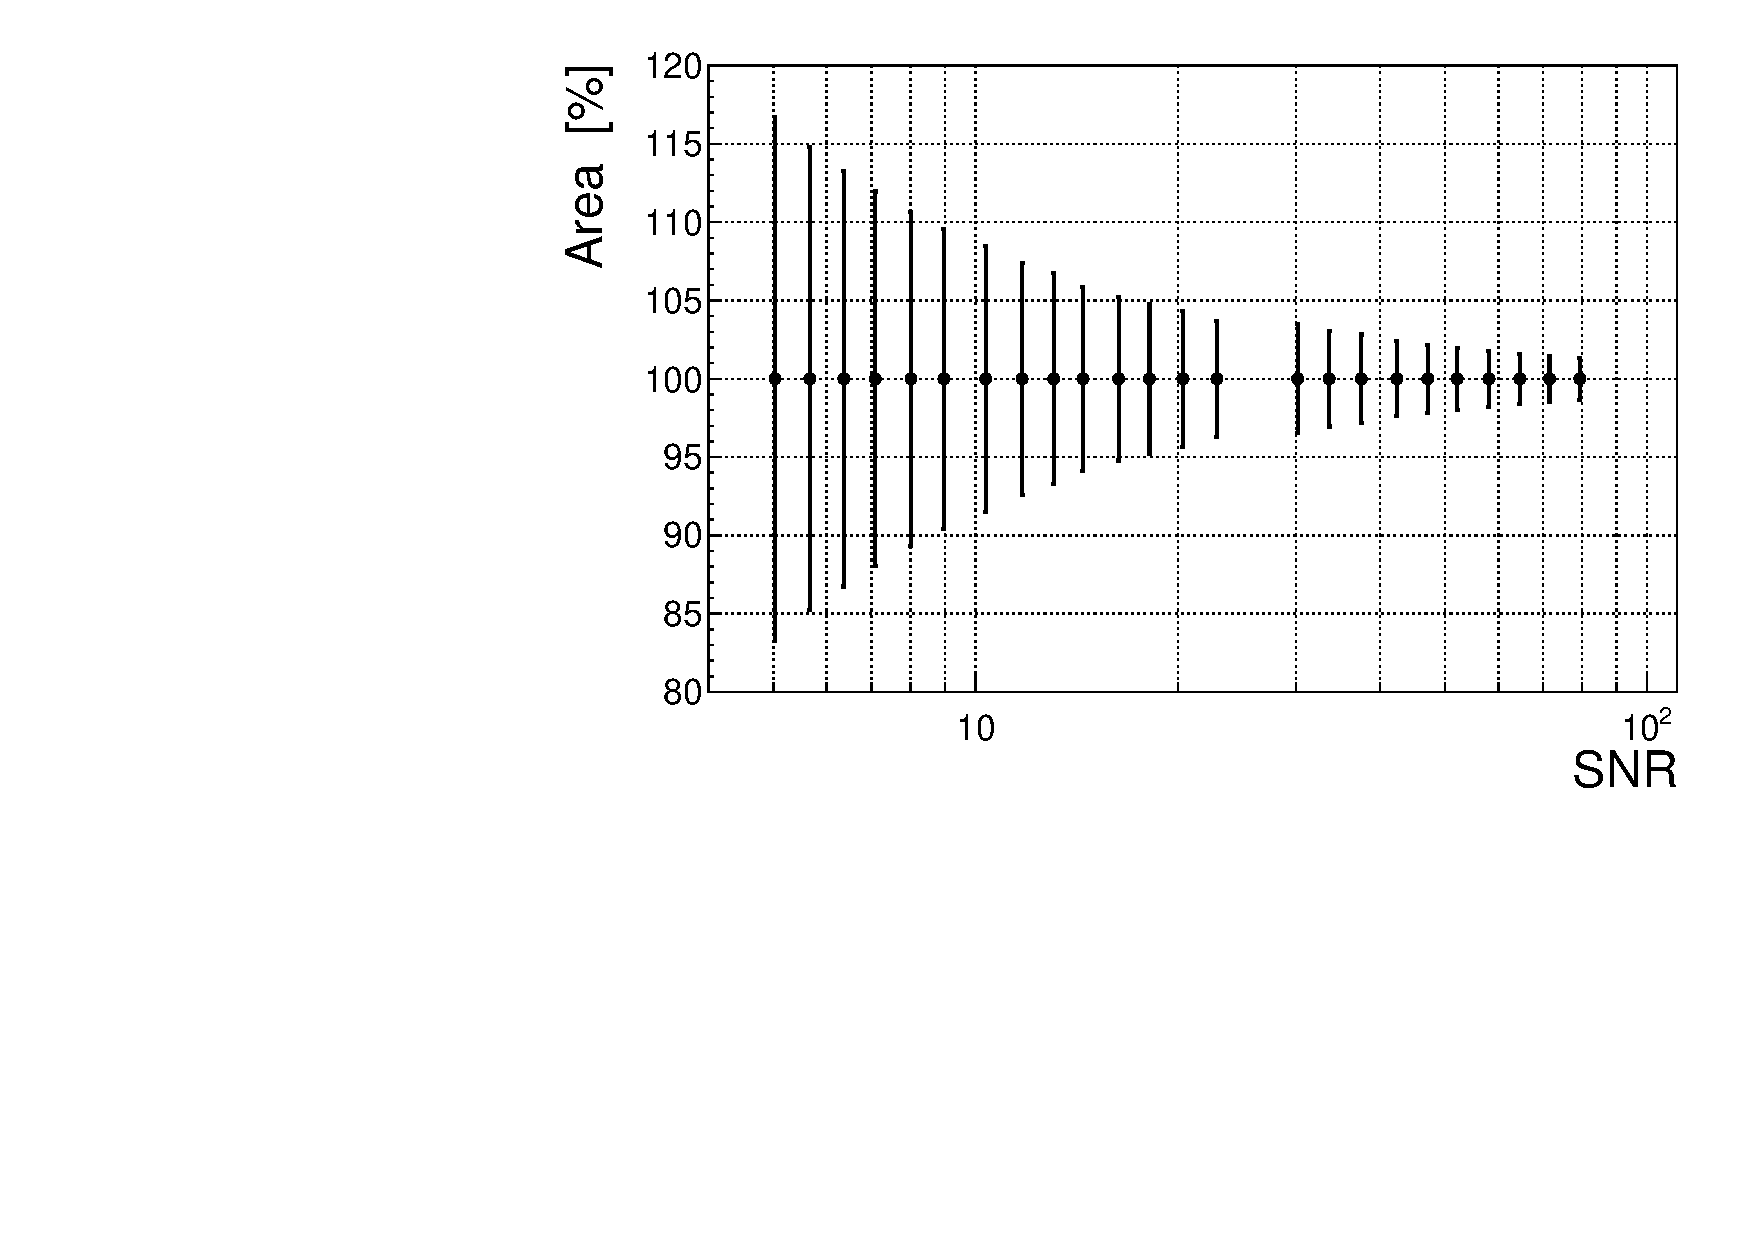
\includegraphics[width=0.47\textwidth]{../scripts/05_current_monitoring/PulseGenTests/plots/snrArea1}  \label{fig:snrArea1}}
\end{tabular}
\caption{These figures show the measurements errors for amplitude (top left), width (top right) and area (bottom left) as a function of the signal-to-noise ratio.}
\label{fig:ratiosnr}
\end{figure}


\subsubsection{Conclusion}
The results show that: 1) the amplitude, area and width measurement are linear for pulses at least 2~ns wide, 2) the highest rate of the PSA algorithm is $\sim6\times10^6$ pulses per second and 3) the lowest SNR where the algorithm still functions is $\sim$5, but the area measurement spread at that SNR is significant.




\subsection{Comparison between the charge-sensitive and current spectroscopy}
The calibration was done using a quadruple-$\upalpha$ source containing \textsuperscript{148}Gd, \textsuperscript{239}Pu, \textsuperscript{241}Am and \textsuperscript{244}Cm. Each of the radioactive elements emits $\upalpha$ particles with a specific energy: 3.2~MeV, 5.2~MeV, 5.5 MeV and 5.8~MeV. The PSA in combination with the CIVIDEC C2 current amplifier was compared against an 8-bit spectroscopic application in combination with the CIVIDEC Cx spectroscopy amplifier.% and a commercial 14-bit spectroscopic readout.

\begin{figure}[!t]
\centering
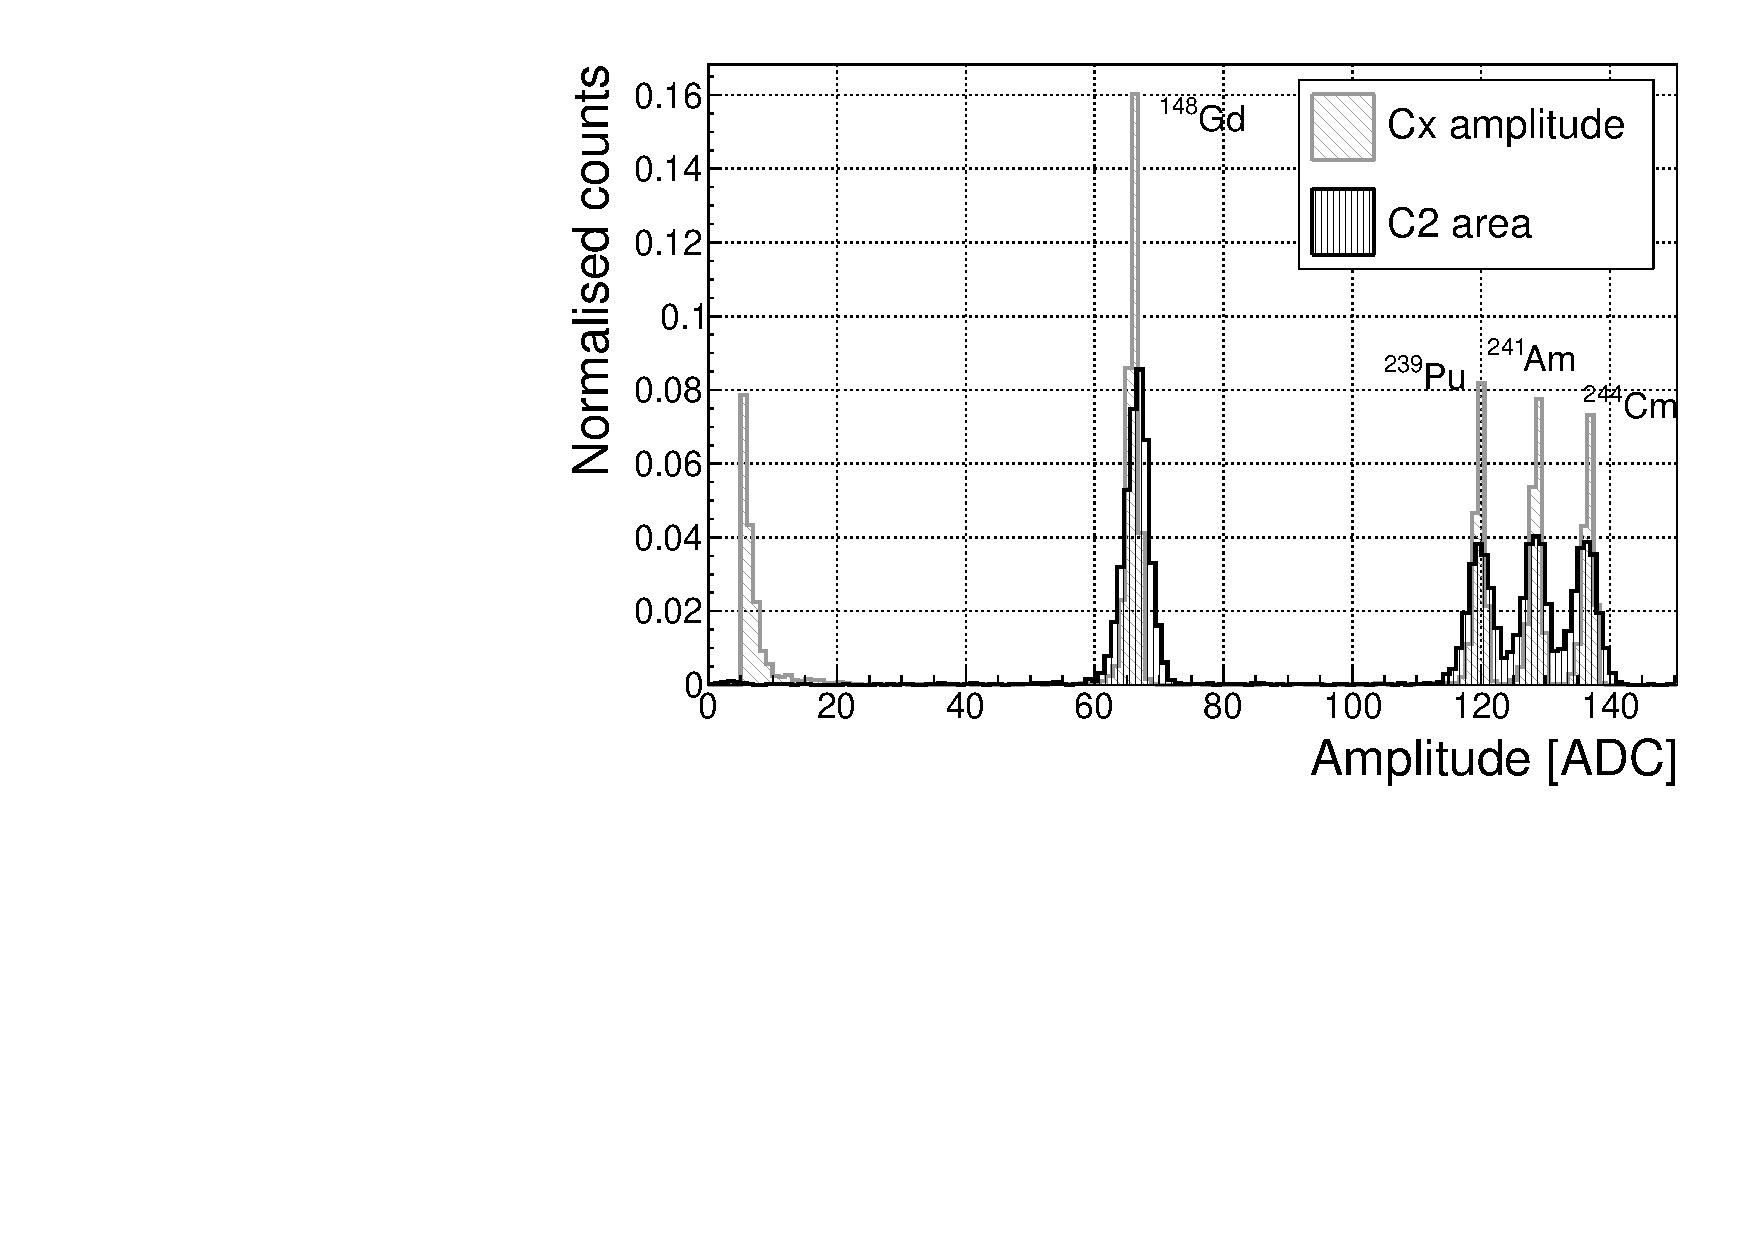
\includegraphics[width=0.7\textwidth]{../scripts/05_current_monitoring/plot4alpha/plots/4alphaCompare}
\caption{Energy spectrum of a quadruple-$\upalpha$ source using a CIVIDEC Cx spectroscopic amplifier and a CIVIDEC C2 current amplifier. The peak on the left part of the Cx distribution is attributed to the $\upgamma$ background.}
\label{fig:c2cx4alpha}
\end{figure}

Figure~\ref{fig:c2cx4alpha} shows the energy spectrum acquired by the two amplifiers. The $^{241}$Am peak measured by the CIVIDEC Cx amplifier has an RMS of 0.8~ADC, which corresponds to a 32~keV energy resolution. For comparison, the CIVIDEC C2 broadband current amplifier measures this peak with an RMS of 1.9~ADC, which corresponds to a 75~keV energy resolution. Therefore the energy spectrum measured by the current amplifier has a factor of 2.3 lower energy resolution.


%\subsection{Pulse identification test}
%The device was tested using two radioactive sources at the same time. The $^{241}Am$ source of 5.12~MeV $\upalpha$ particles was placed on one side of the diamond. The $^{60}$Co source of photons with the energy of 1.3~MeV was placed on the other side. The diamond was put in the vacuum chamber to reduce the energy loss of $\upalpha$ particles in the air. The chamber also provided good shielding, reducing the noise pick-up significantly. 
%alpha and cobalt







% ---------------------------------------------------------------------------------------------------------------
%\clearpage
\section{Source calibration}
\label{sec:sourcecalib}
% ---------------------------------------------------------------------------------------------------------------

\subsection{Pulse classification}
\label{sec:radclass}

Pulses induced by a specific radiation type have a specific pulse shape and therefore similar parameters. This section outlines the parameter space for several types of radiation. Table~\ref{tab:class} lists the types of radiation and their respective pulse shapes. The  types have been sorted into classes for easier discussion. The table includes the radioactive sources that emit these particles. 

\begin{footnotesize}
\begin{center}
\begin{tabular}{l c c c c c c c}
\hline
Class & Particle type & Current signal & Source   \\
\hline
A & $\upalpha$        & Square pulse, h$^-$ drift & $^{241}$Am  \\
B & $\upalpha$        & Square pulse, e$^-$ drift & $^{241}$Am   \\
C & $\upbeta$         & Triangular pulse               & $^{90}$Sr  \\
D & $\upgamma$    & Triangular pulse               & $^{60}$Co   \\
E & n                       &  Mixed pulse shapes        & $^{239}$Pu  \\
F & p                       & Mixed pulse shapes         & $^{239}$Pu  \\ 
\hline
\end{tabular}
\captionof{table}{Current pulse classification.}
\label{tab:class}
\end{center}
\end{footnotesize}


%\clearpage

\begin{figure}[h]
\centering
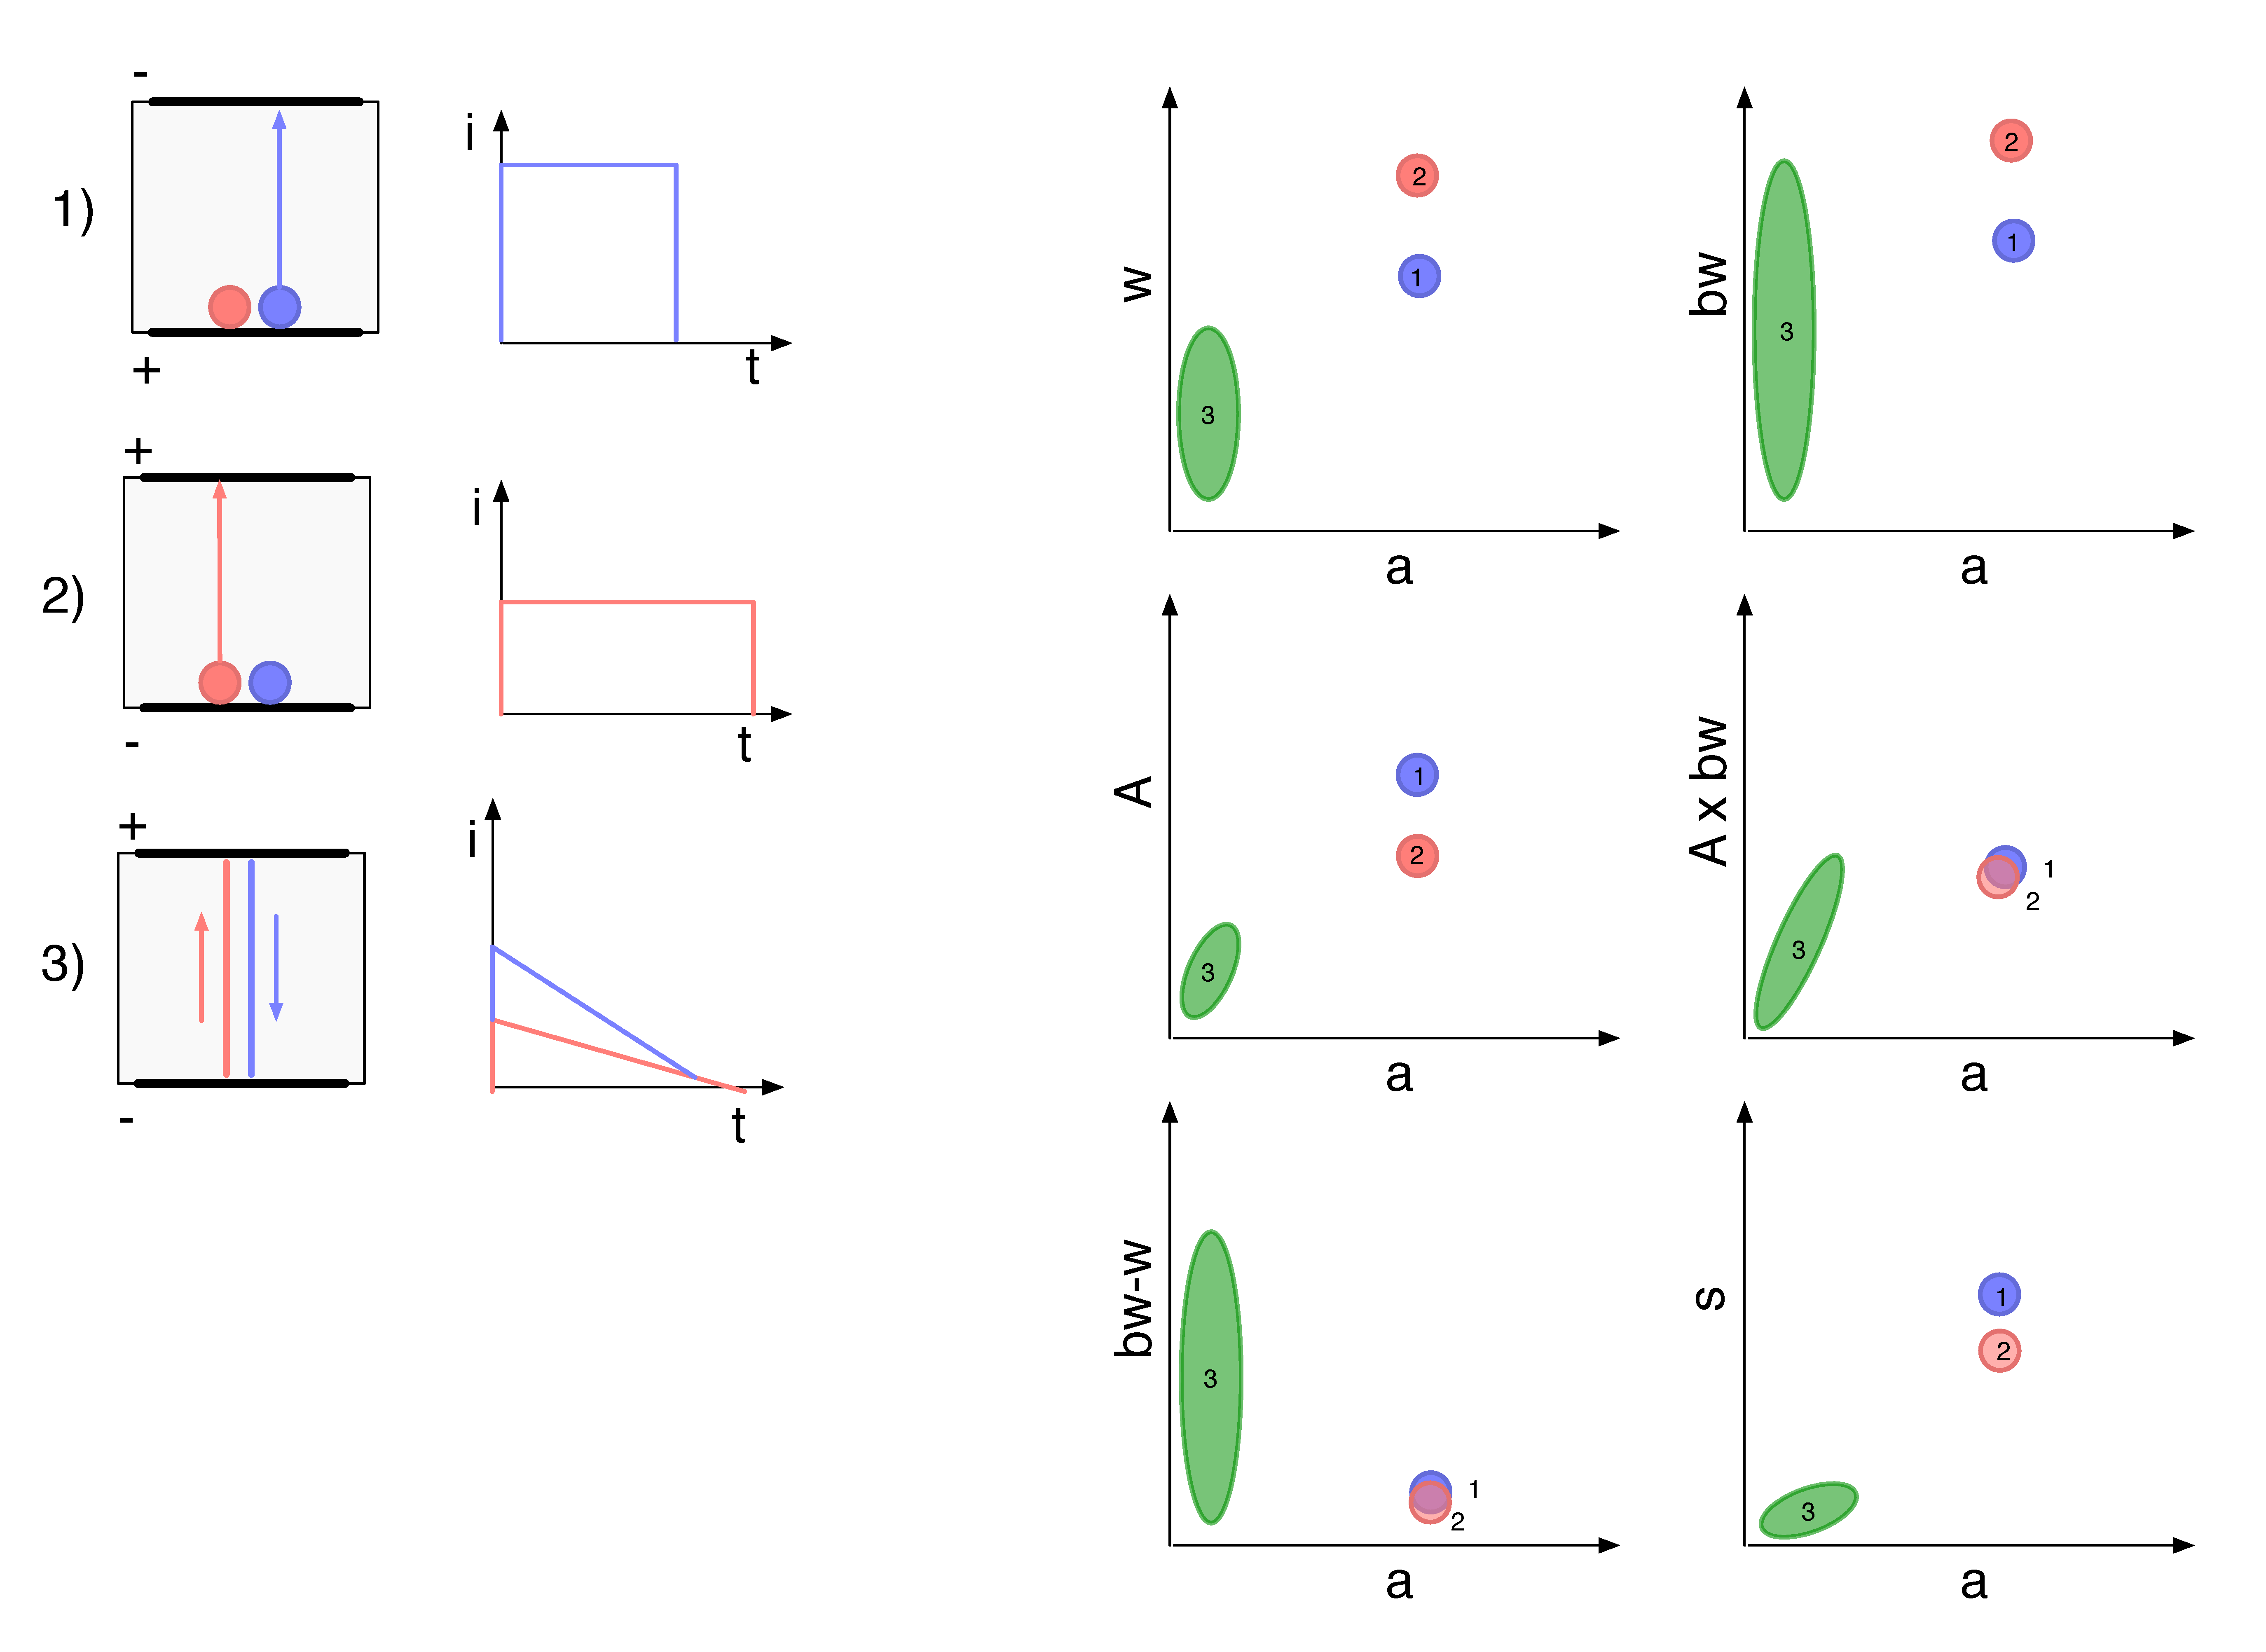
\includegraphics[width=0.9\textwidth]{05_current_monitoring/plots/classABCD}
\caption{Class A, B, C, D.}
\label{fig:classabcd}
\end{figure}
\clearpage
\subsubsection{Class A, B, C, D}
\label{sec:classabcd}%$\upalpha$ and $\upbeta$ pulses have been discussed in previous chapters. 
An $\upalpha$ particle deposits all its energy at the point of entry in the sensor. Depending on the polarity of the sensor bias voltage, either holes or electrons drift through the sensor, inducing a rectangular current pulse. 

Schematic 1) in figure~\ref{fig:classabcd} shows the positive charge carriers drifting through the sensor and the current pulse they induce -- Class A. Holes produce a short and high rectangular pulse. The parametric ``fingerprint'' of these current pulses is shown on the right side of figure~\ref{fig:classabcd}, marked with number 1. All $\upalpha$ particles deposit the same amount of charge.
%Most $\upalpha$ particles deposit the same amount of charge, except for those that lose some of their energy in the air or in the sensor's electrode. Therefore the area distribution peaks at a specific area value and has a tail towards the lower area values. 
The width and the base width are always the same as the drift velocity of the charge carriers does not change regardless of the number of carriers drifting. The base value is slightly higher due to the rise and fall time of the current signal. The amplitude is the same for all pulses. The same goes for the calculated area (a product of the amplitude and base value). For an ideal pulse, the coefficient between the measured area and the calculated area for a rectangular pulse is 1. The difference between the base width and the width is close to 0 and depends on the rise and fall time of the current signal defined by the electronics. The falling slope of the signal depends on the amplitude of the signal, therefore it is constant for a nominal pulse. 

Schematic 2) in figure~\ref{fig:classabcd} shows the negative charge carriers drifting through the sensor and the current pulse they induce -- Class B. Electrons produce a wide and low rectangular pulse. Parametrically Class B differs from Class A in the width, base width, amplitude and slope. The former two are higher due to a lower drift velocity of electrons. The amplitude is proportionally higher to preserve the constant pulse area due to a constant deposited charge.

Schematic 3) in figure~\ref{fig:classabcd} shows the configuration of the deposited charge created by an incident $\upbeta$ particle -- Class C. The positive and negative charge carriers induce a triangular pulse while drifting to their respective electrodes. The number of electrons and holes created differs from pulse to pulse, but follows a Landau distribution, as discussed in previous chapters. The amplitude of the pulse is linearly dependent on the initial number of created carriers, but has a higher coefficient than that of Class A or B. The same goes for the width and base width. The width of the pulses is lower than that of Class A and B. The base width, however, can already be close to Class A and B for the widest Class C pulses. The coefficient between the measured and calculated area is close to 2. The difference between the base width and width is a wide distribution. The falling slope is a low value for triangular pulses of all amplitudes.

$\upgamma$ particles interact with the diamond mostly via the photoelectric effect and via Compton scattering, exciting an electron, which in turn ionises the sensor. Therefore the predicted pulse shape -- Class D -- will be similar to that of $\upbeta$ particles -- Class C. 




%travel 30~\% faster than electrons at room temperature and create a narrower and higher pulse. The area is equal for both pulses. 

\clearpage

\begin{figure}[!t]
\centering
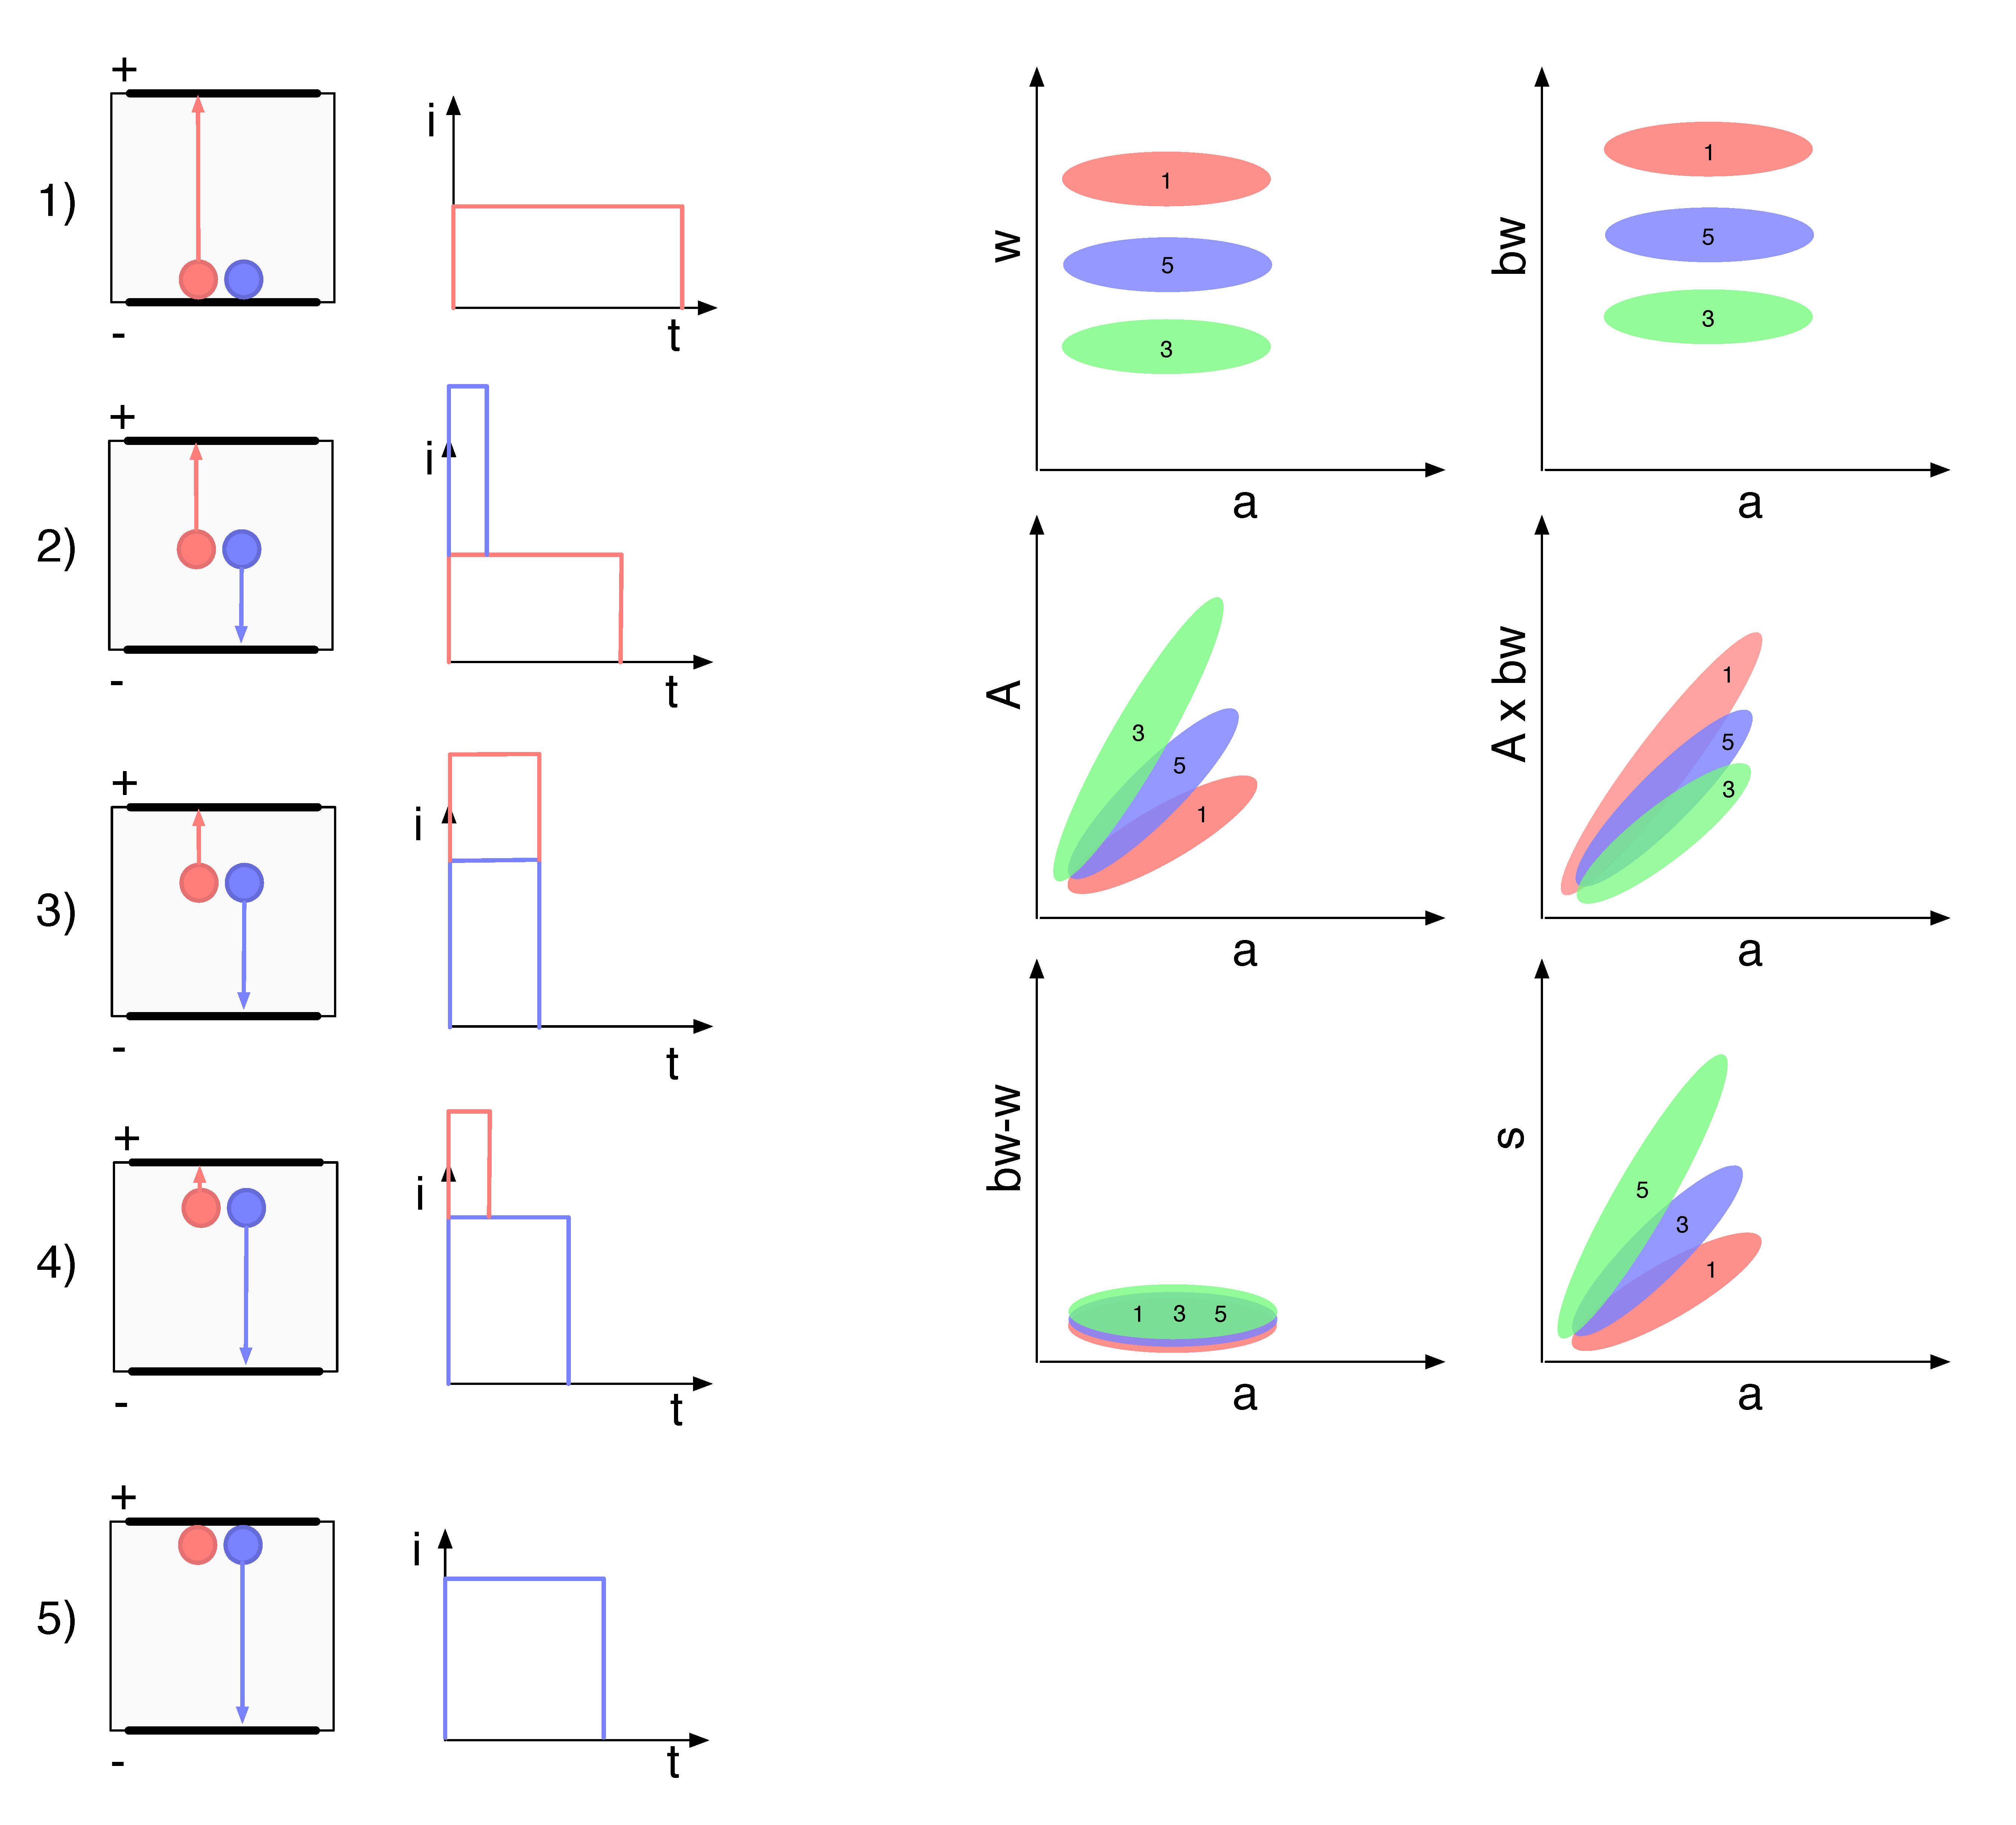
\includegraphics[width=0.9\textwidth]{05_current_monitoring/plots/classE}
\caption{Class E.}
\label{fig:classe}
\end{figure}

\clearpage
\subsubsection{Class E}
\label{sec:classe}
Neutrons interact with the core of the carbon atoms, producing a range of particles ranging from $\upgamma$, $\upbeta$ and $\upalpha$ to protons. Neutrons are therefore a source of Class A, B, C, D, E and F pulses. Class E is a special case whereby $\upalpha$ particles are created at various points throughout the sensor. These particles immediately deposit all their energy and the created electrons and holes that drift to their respective electrodes induce a pulse with a specific shape. Schematics in figure~\ref{fig:classe} show examples of an $\upalpha$ creation in the sensor at five depths. 

Schematics 1) and 5) are equal to Class B and A type. The difference here is that the created $\upalpha$ particles have a range of energies and therefore the deposited charge has a wide range. Their parametric fingerprint is similar to that of Class A and B, but is now spread over a wide range. The width and base width are equal across the measured range, the same holds for the difference between base width and width. The amplitude for both 1 and 5 increases linearly with the area.

Schematic 2) shows a carrier creation in the middle of the sensor and its respective current pulse. The holes drift faster and reach their respective electrode before the electrons reach the opposite side. The resulting pulse has a high peak at the start where both charges contribute to the signal and a long rectangular tail pertaining to the electron drift. Schematic 4) is similar to 2), with a difference that in this case the electrons contribute to the initial peak. These two cases are not shown in the parameter space.

Schematic 3) shows a special case in which the created electrons and holes reach their respective electrodes at the same time. This results in a short and high rectangular shaped current pulse. It is narrower than 1) and 5). Its amplitude increase as a function of the area is faster than for the other two. The same goes for the slope. Inversely, the calculated area increase as a function of the area is slower due to a narrower base width. 

In summary, Class E pulses stem from neutron interactions at the electrodes or in the bulk, forming three distinct lines.





\clearpage

\begin{figure}[!t]
\centering
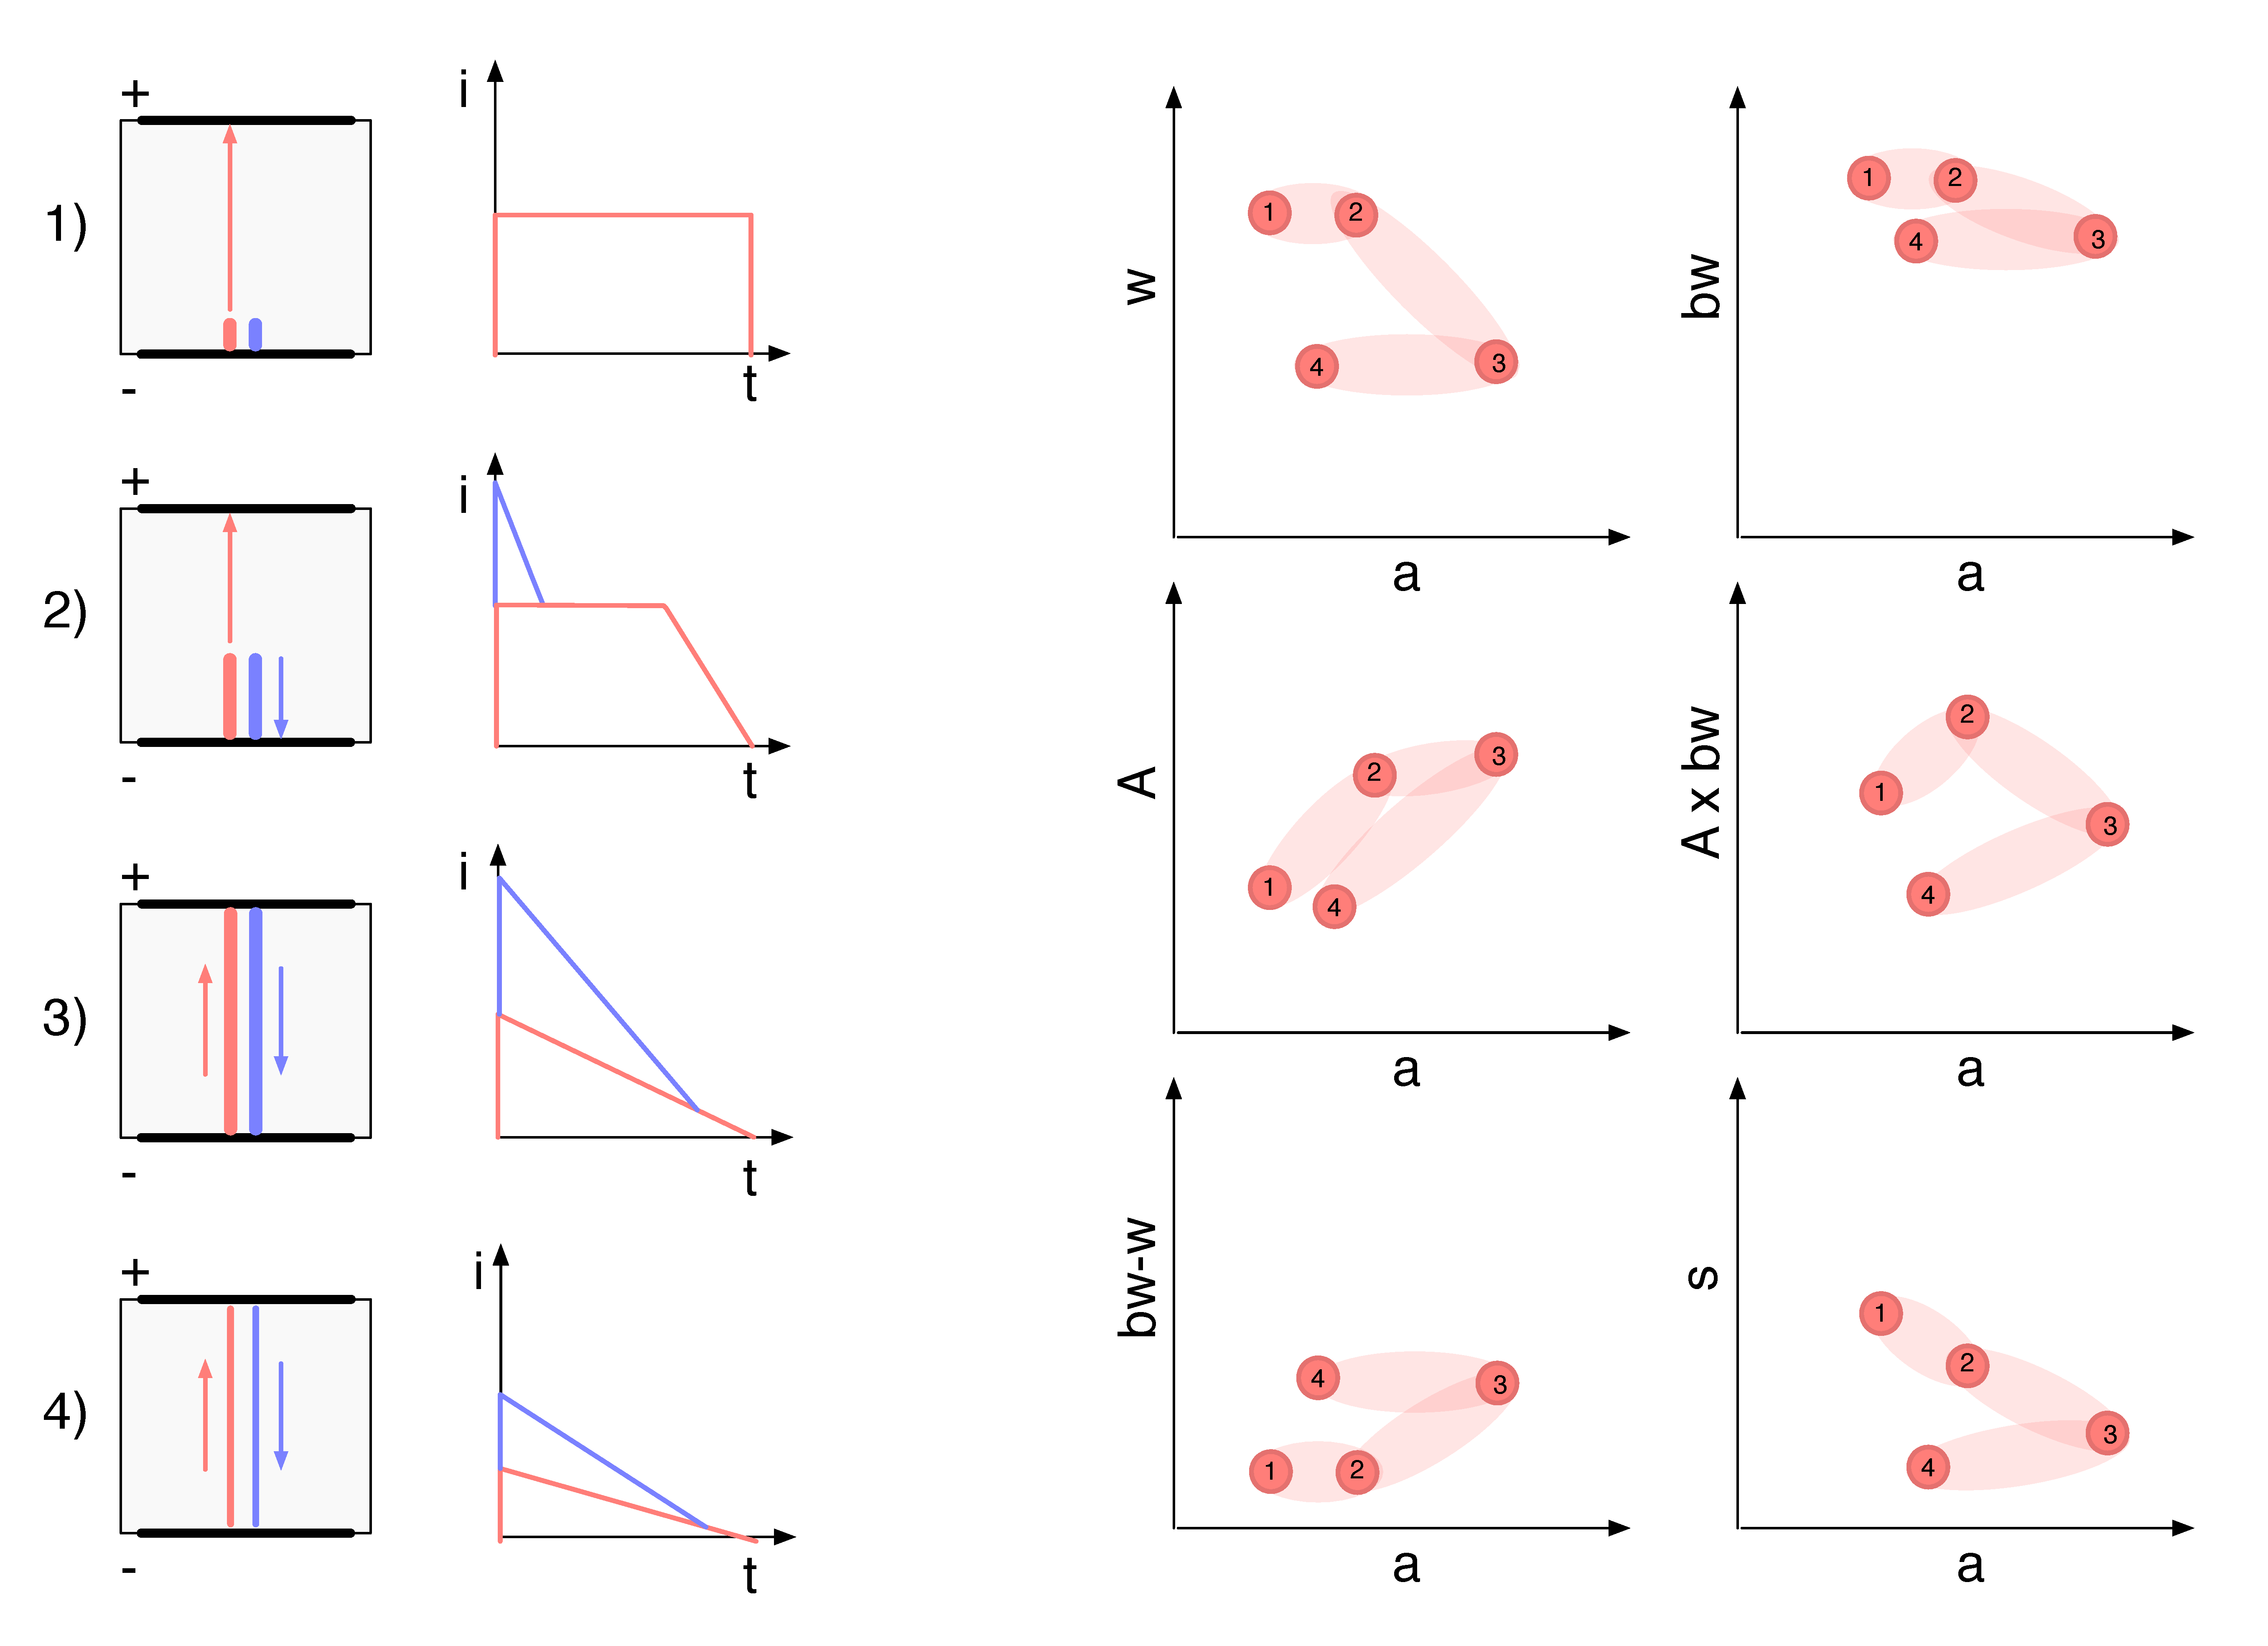
\includegraphics[width=0.9\textwidth]{05_current_monitoring/plots/classF}
\caption{Class F. Red points in the graphs marked 1, 2, 3 and 4 correspond to example pulses on the left.}
\label{fig:classf}
\end{figure}

\clearpage
\subsubsection{Class F}
\label{sec:classf}

Protons can produce a range of pulse shapes, depending on their energy. High-energy MIPs fly through the sensor and produce a triangular pulse equal to that of $\upbeta$. Those with a low energy get stopped in the sensor, inducing a pulse with a complex shape. Class F comprises protons created by a neutron interaction with a carbon atom, referred to as recoil protons. For reasons of clarity the examples shown below stem from a neutron interaction at the negatively charged electrode. In addition, the direction of the recoil proton is always in the direction of the opposite electrode.

Schematic 1) shows a creation of a low-energy recoil proton. It deposits all its energy within a few $\upmu$m, inducing a Class B rectangular pulse. It also resembles the Class B in the parameter space.

Schematic 2) shows a proton that travels for a third of the sensor width before being stopped. The trace it leaves induces a pulse with an initial peak due to the contribution of the drifting holes and a gentle falling edge at the end. Its width and base width are still close to the nominal value. The amplitude is significantly higher due to the initial peak. As a consequence, the calculated area is higher as well. The difference between the base width and width is still nominal. The slope value decreases due to a less pronounced falling edge of the pulse.

Schematic 3) shows a corner case whereby the recoil proton is stopped at the opposite electrode. It induces a high triangular pulse. Its width is significantly lower due to the high amplitude. The base width, however, remains almost the same. Therefore the difference between the base width and width increases. The slope continues decreasing.

Schematic 4) shows a high-energy recoil proton that exits the sensor with a high velocity. According to the Bethe-Bloch such a highly energetic particle deposits less charge than that with a low energy. The resulting current pulse therefore has a lower amplitude while preserving the width. Its slope is also lower due to the lower amplitude.


\subsection{Data acquisition}
The operation of the pulse shape analysis has been tested using several radioactive sources. In particular, an $\upalpha$, a $\upbeta$ and a $\upgamma$ source have been used. Each source has been placed on top of the diamond detector and left for a predefined time depending on its activity. Table~\ref{tab:semicompare} shows the sources used, the time of exposure and their rate during data acquisition. The data for the $\upalpha$ source have been taken for both polarities. 
%In addition, a long run with an $\upalpha$ source with a sheet of paper in between the source and the diamond has been taken. The paper stops the $\upalpha$ particles but lets through the photons, which helps to estimate the background photon radiation of the source.

\begin{footnotesize}
\begin{center}
\begin{tabular}{l c c c c c c c}
\hline
Run & Source & Radiation & Energy [MeV] & Time [h]  & Triggers & Rate [s$^{-1}$]  & Bias [V]   \\
\hline
%1&$^{241}$Am*  & $\upalpha$ & 5.5 & 60 & 958 & 4.4e-3  & 500 \\
1&$^{241}$Am  & $\upalpha$ & 5.5 & 17 & 10558 & 0.17  & 500 \\
2&$^{241}$Am  & $\upalpha$ & 5.5 & 18 & 11454 & 0.18 & -500 \\
3&$^{90}$Sr  & $\upbeta$ & 2.3 & 0.42 & 1.07e6 & 1'000 & 500 \\
4&$^{60}$Co  & $\upgamma$ & 1.3 & 0.28 & 1.34e6 & 3'300 & 500 \\
5&$^{239}$Pu~Be  & $n$ & 1--10 & 2.5 & 1.5e6 & 230 & 500 \\ 
\hline
\end{tabular}
\captionof{table}{Measurements carried out at Atominstitut.}
\label{tab:sources}
\end{center}
\end{footnotesize}

% ATI source measurements
\clearpage
\begin{figure}[!t]
%\centering
\begin{tabular}{rrr}
%\subfloat[$^{241}$Am background.]{\includegraphics[width=0.44\textwidth]{../../../CIVIDEC/dataRead/data/plots/reportATI/27-pulse-background-1} \label{fig:am1}} &
\subfloat[$^{241}$Am, e$^{-}$ collection.]{\includegraphics[width=0.44\textwidth]{../../../CIVIDEC/dataRead/data/plots/reportATI/10-pulse-alpha-e-0}  \label{fig:am2}} &
\subfloat[$^{241}$Am, h$^+$ collection.]{\includegraphics[width=0.44\textwidth]{../../../CIVIDEC/dataRead/data/plots/reportATI/18-pulse-alpha-h-0}  \label{fig:am3}} \\
\subfloat[$^{90}$Sr.]{\includegraphics[width=0.44\textwidth]{../../../CIVIDEC/dataRead/data/plots/reportATI/13-pulse-beta-0} \label{fig:sr1}} &
\subfloat[$^{60}$Co.]{\includegraphics[width=0.44\textwidth]{../../../CIVIDEC/dataRead/data/plots/reportATI/12-pulse-gamma-0}  \label{fig:co1}} \\
\subfloat[$^{239}$Pu~Be.]{\includegraphics[width=0.44\textwidth]{../../../CIVIDEC/dataRead/data/plots/reportATI/15-pulse-neutron-0}  \label{fig:pu1}} 
\end{tabular}
\caption{Accumulated current pulses for all runs.}
\label{fig:accpulses}
\end{figure}
\clearpage
%The pulses acquired during the data taking are shown in persistence plots in figures~\ref{fig:accpulses}. 
%Figure~\ref{fig:am1} showing the $^{241}$Am source background reveals that the diamond detector had been contaminated, probably with chipped-off grains of the unsealed source. This stems from the fact that $\upalpha$ pulses are recorded despite having a sheet of paper, which stops all the particles emitted by the source. 
%However, the number of $\upalpha$ hits due to contamination is negligible - an estimated 1~h$^{-1}$. 
Figure~\ref{fig:accpulses} shows five sets of data acquired by a non-irradiated diamond sensor. The measurements were carried out in the following order: a), c), d), e), b).

Figure~\ref{fig:am2} shows a set of current pulses induced by the $\upalpha$ particles whereby only the electrons drift through the sensor. The great majority of particles creates a defined number of charge carriers. According to the FWHM of the pulse, the electrons drift for 9~ns before reaching the opposite electrode. The pulse amplitude is stable during the drift, with a gentle positive inclination. This hints on a weak negative space-charge built up across the sensor. Some pulses have a lower amplitude while retaining the width; the smaller pulse area means that there are fewer drifting charge carriers than a nominal value. This shows that some incident $\upalpha$ already lose a part of their energy while traveling through the air before hitting the sensor. Furthermore, there is a number of low-amplitude triangular pulses which are created by incident $\upgamma$ particles. Finally, the scarce entries above the baseline after the pulse stem from interference pulses.

Figure~\ref{fig:am3} also shows the $\upalpha$-induced current signals, but for the hole collection. The number of holes created is equal to the number of created electrons, therefore the collected charge is the same for both. This means that the area of the current pulse is equal to that in figure~\ref{fig:am2}. The pulses are only 6~ns wide, which confirms that hole mobility in diamond is $\sim$30~\% higher than that of electrons at room temperature. Therefore the current pulse must be higher to preserve the area. The pulses have a steep negative droop. This is due to a strong negative space-charge built up during preceding measurements with a neutron source. Furthermore, some pulses induced by a lower energy $\upalpha$ have a lower amplitude and hence a lower pulse area. Finally, the $\upgamma$-created triangular pulses are still present. 

Figure~\ref{fig:sr1} shows the triangular pulses created by the incident $\upbeta$ particles. Most have a low amplitude that is close to the trigger threshold (red coloured line). Those below the threshold are not visible by the PSA. The entries behind the pulses are either interference pulses or $\upbeta$ pulses following the first pulse.

Figure~\ref{fig:co1} shows the triangular pulses created by the incident $\upgamma$ particles. The distribution is very similar to that created by the incident electrons in figure~\ref{fig:sr1}. This is expected -- $\upgamma$ particles interact with the sensor via compton scattering, freeing an electron which in turn ionises the sensor. Therefore the resulting current pulses of an incident $\upgamma$ are similar to those of an incident $\upbeta$.

Figure~\ref{fig:pu1} shows that the neutron source causes the widest variety of pulse shapes - triangular and rectangular as well as those in between. This stems from the various interactions of neutron with carbon atoms, whereby $\upalpha, \upbeta, \upgamma$ or protons can be produced. The prevailing pulses are still those created by $\upgamma$. %The area spectrum is also significantly higher than that of all previous radiation types.  
Pulse shapes caused by neutrons are described in detail in~\cite{PAVEL:00003, CHRISSI:00005}. 


%Another point worth noting is the falling slope of the rectangular pulse in figure~\ref{fig:am3}. This stems from the space charge that had built up during the neutron irradiation. %and is discussed in section~\ref{sec:spacecharge}. 





\subsection{Scatter plots}
The parameters of the pulses are plotted in 2D histograms - in form of scatter plots. The energy spectrum is directly proportional to the measured area of the current pulses, therefore all the parameters are plotted as a function of the pulse area.

Every individual parameter can be attributed a set of qualifiers with which a certain part of the distribution can be rejected. There are two ways to apply the qualifiers. One is to set the minimum and maximum value for a specific parameter. The accepted pulses are those in between these two values. The minimum and the maximum qualifier are marked with a blue and a red line in the subsequent scatter plots. The second way is to apply a linear cut to the distribution in the scatter plot. The user can choose the slope of the line and to accept either the pulses above or below the line. The colour of the line is blue if the part above the line is accepted and red if opposite. Currently two scatter plots have this option implemented: area vs amplitude and area vs amplitude$\times$base width. The latter represents the Form Factor, which is discussed in section~\ref{subsec:algorithm}.

%The sets of plots in figures~\ref{fig:scatterae}, \ref{fig:scatterah}, \ref{fig:scattersr} and \ref{fig:scatterco} show the above listed parameters plotted as a function of the pulse area for $^{241}$Am (electrons and holes), $^{90}$Sr and $^{60}$Co source, respectively. Any distinguishable difference between the plots of two sources would suggest that that particular parameter can be used to distinguish one type radiation from the other. 
%For the most part the $\upgamma$ are considered the rejected pulses (greyscale colour palette) whereas $\upalpha$ particles or neutrons are accepted (yellow colour palette). In special cases only a certain types of neutron interactions are accepted, as depicted in section~\ref{sec:nm}.


 

% alpha: gamma background. alphas of all energies (air).
% gamma, beta - overlapping
%\clearpage
%\begin{figure}[!t]
%\centering
%\includegraphics[width=0.99\textwidth]{../../../CIVIDEC/dataRead/data/plots/reportATI/29-scatter-0}
%\caption{Background measurements}
%\label{fig:scatterbm}
%\end{figure}
\clearpage
\begin{figure}[!t]
\centering
\includegraphics[width=0.99\textwidth]{../../../CIVIDEC/dataRead/data/plots/reportATI/18-scatter-10-add}
\caption{$^{241}$Am, h$^{+}$ collection. Qualifiers: FWHM, amplitude, calculated area.}
\label{fig:scatterah}
\end{figure}

\clearpage
\subsubsection{$^{241}$Am source, h$^+$ collection}
\label{sec:amsrch}
The source emits $\upalpha$ particles at $\sim$5.5~MeV and 60~keV $\upgamma$ photons. Due to the losses in the air and in the electrode the measured $\upalpha$ energy varies -- between $\sim$5~MeV down to 1~MeV.  Figure~\ref{fig:scatterah} shows the parameter space of the acquired data for hole collection - Class A . Width, amplitude and calculated area qualifiers have been used to identify the $\upalpha$ pulses and reject the $\upgamma$. Figure~\ref{fig:1dalphaareah} shows a one-dimensional area distribution of the acquired data. The MPV of the $\upgamma$ distribution is not at the expected position (30~pVs, which is approximately a factor of 20 lower than the $\upalpha$ peak). This is due to two factors: increased non-linearity in area measurement at the lower range as shown in figure~\ref{fig:ratiorange} and the fact that the threshold for self-triggering cuts the majority of the Landau distribution due to the low amplitude of the pulses. The effect is also observed in $\upgamma$ source measurements in section~\ref{sec:gammasrc}.
\begin{description}
\setlength\itemsep{-0.3em}
\item[Width: ] A distinct horizontal line at 6.5~ns starting from 100 and peaking at 600~pVs shows the aforementioned spread of $\upalpha$ energies. The width of the pulse remains constant. $\upgamma$ cluster overlaps with the $\upalpha$ cluster at low energies. Width qualifier is used.
\item[Base width: ] Wider than the FWHM, yet still constant over the entire range. High overlap with $\upgamma$.
\item[Amplitude: ] Linear increase with area. The coefficient for $\upalpha$ pulses is lower than that for $\upgamma$. Amplitude qualifier is used.
\item[Calculated area: ] Barely distinguishable difference in slope coefficients for $\upalpha$ and $\upgamma$. Calculated area qualifier is used.
\item[Base width -- width: ] Minimal difference for $\upalpha$, high spread for $\upgamma$ as expected. At low $\upgamma$ area the overlap is high, so the qualifier cannot be used.
\item[Slope: ] Linear increase with the area. Significant overlap in the low area range. A line of entries with a high slope at low area pertains to short noise pulses with a high spike.
\end{description}
\begin{figure}[]
\centering
\includegraphics[width=0.7\textwidth]{../../../CIVIDEC/dataRead/data/plots/reportATI/10-area-0}
\caption{$^{241}$Am area histograms for hole collection. The green histogram represents all collected data whereas the red one marks the data whereby the pulse parameters are within the qualifiers. The $\upalpha$ peak at 600~pVs is clearly visible, followed by a $\upgamma$ quasi-Landau distribution with an MPV of $\sim$70~pVs and a noise peak at the very left of the area distribution. These two contributions have been rejected by the qualifiers.}
\label{fig:1dalphaareah}
\end{figure}
%The shape of the pulse from this type of radiation retains the width even at smaller energies. Only its amplitude is decreased. This is because the free charge carriers in the diamond are traveling with the same speed in all cases, inducing rectangular pulses of the same widths. 
%
%The other cluster in the [area, FWHM] space comes from the background $\upgamma$. The two clusters are far apart from one another with no overlap. It is therefore straightforward to define a cut in the FWHM to distinguish between the $\upalpha$ and $\upgamma$ entries. This is done by means of the minimum and maximum FWHM constant qualifier, which marked red and blue in the [area, FWHM] subfigure.
%
%The [area, amplitude] subfigure also reveals two distinguishable clusters, which can be segregated using a linear qualifier. The angle of the $\upalpha$ stripes in the [area, amplitude] subplots is significantly smaller than that of the photon stripe. The separation is much less pronounced in the other subfigures. 
%
%There is a third barely distinguishable island visible in the top two plots, both area and width values close to zero. This island is formed by noise, which triggered the analysis.
%
%The situation is similar when inverting the bias voltage and collecting holes, as shown in figure~\ref{fig:scatterah}. Here, however, the two clusters are much closer together even in the [area, FWHM] subfigure. This makes it more difficult to define a clear border between the two. The other five qualifiers are in this case less important than the FWHM. Nevertheless, it can be deduced from the plots that the difference BW-FWHM must be below 4~ns.
%
%The slope is dependent of the amplitude, which can be seen in the bottom right plot, making it an unreliable qualifier in the lower area range. The amplitude, scaling with area, makes a distinguishable straight line in the middle left subfigure. 
%
%The amplitude increase with area in the [area, amplitude] subfigure is similar for $\upgamma$ and $\upalpha$ particles. Therefore a linear qualifier can not be used to distinguish $\upalpha$ radiation from $\upgamma$ radiation when measuring holes.


\clearpage
\begin{figure}[!t]
\centering
\includegraphics[width=0.93\textwidth]{../../../CIVIDEC/dataRead/data/plots/reportATI/10-scatter-10-add}
\caption{$^{241}$Am, e$^{-}$ collection. Qualifiers: FWHM, amplitude, calculated area.}
\label{fig:scatterae}
\end{figure}


\clearpage
\subsubsection{$^{241}$Am source, e$^-$ collection}
Figure~\ref{fig:scatterae} shows the parameter space of the acquired data for electron collection - Class B. Width, amplitude and calculated area qualifiers have been used to identify the $\upalpha$ pulses and reject the $\upgamma$. Figure~\ref{fig:1dalphaareae} shows a one-dimensional area distribution of the acquired data. The $\upgamma$ MPV of 70~pVs is not as expected (30~pVs); the reason for the shift is discussed in section~\ref{sec:amsrch}.
\begin{description}
\setlength\itemsep{-0.3em}
\item[Width: ] A distinct horizontal line at 8.5~ns starting from 100 and peaking at 600~pVs shows the spread of $\upalpha$ energies. The width of the pulse remains constant. $\upgamma$ cluster does not overlap with the $\upalpha$ cluster at low energies as none of the $\upgamma$ pulses are as wide as the $\upalpha$. Width qualifier is used.
\item[Base width: ] Wider than the FWHM, yet still constant over the entire range. Small overlap with $\upgamma$.
\item[Amplitude: ] Linear increase with area. The coefficient for $\upalpha$ pulses is significantly lower than that for $\upgamma$, also lower than that for hole collection. Amplitude qualifier is used.
\item[Calculated area: ] Distinguishable difference in slope coefficients for $\upalpha$ and $\upgamma$. Calculated area qualifier is used.
\item[Base width -- width: ] Minimal difference for $\upalpha$, high spread for $\upgamma$ as expected. At low $\upgamma$ area the overlap is low, but due to low statistics.
\item[Slope: ] Linear increase with the area. Overlap in the low area range. A line of entries with a high slope at low area pertains to short noise pulses with a high spike.
\end{description}

\begin{figure}[]
\centering
\includegraphics[width=0.7\textwidth]{../../../CIVIDEC/dataRead/data/plots/reportATI/18-area-0}
\caption{$^{241}$Am area histograms for electron collection. The green histogram represents all collected data whereas the red one marks the data whereby the pulse parameters are within the qualifiers. The $\upalpha$ peak at 600~pVs is clearly visible, followed by a $\upgamma$ quasi-Landau distribution with an MPV of $\sim$70~pVs and a noise peak at the very left of the area distribution. These two contributions have been rejected by the qualifiers.}
\label{fig:1dalphaareae}
\end{figure}




\clearpage
\begin{figure}[]
\centering
\includegraphics[width=0.99\textwidth]{../../../CIVIDEC/dataRead/data/plots/reportATI/13-scatter-10}
\caption{$^{90}$Sr scatter plots.}
\label{fig:scattersr}
\end{figure}

\clearpage
\subsubsection{$^{90}$Sr source}
Figure~\ref{fig:scattersr} shows the parameter space of the acquired data for $\upbeta$ particles - Class 3. Figure~\ref{fig:1dsrarea} shows a one-dimensional area distribution of the acquired data. 
\begin{description}
\setlength\itemsep{-0.3em}
\item[Width: ] The width of the $\upbeta$ cluster is spread over a wide range and is not linearly dependent on the area. This implies that the pulse shapes are not necessarily triangular but have varying shapes.
\item[Base width: ] Wider than the FWHM with a similar distribution.
\item[Amplitude: ] Linear increase with the area. A line of entries with a high slope at low area pertains to short noise pulses with a high spike.
\item[Calculated area: ] Linear increase with area.
\item[Base width -- width: ] A wide spread of entries.
\item[Slope: ] A gentle linear increase with the area. A line of entries with a high slope at low area pertains to short noise pulses with a high spike.
\end{description}


\begin{figure}[]
\centering
\includegraphics[width=0.7\textwidth]{../../../CIVIDEC/dataRead/data/plots/reportATI/13-area-0}
\caption{Area histogram for $\upbeta$ particles. Relative to the 600~pVs $\upalpha$ peak, the expected MPV of a $\upbeta$ MIP is $\sim$30~pVs, which is not the case in these distributions (peaking at 60~pVs). This is because the PSA device is a self-triggering system, which cuts the lower energetic particles with the trigger threshold. The resulting distribution is therefore only the top part of the real Landau distribution. This is a limitation of the device, governed by the analog noise of the current pre-amplifier.}
\label{fig:1dsrarea}
\end{figure} 
 
 
\clearpage
\begin{figure}[]
\centering
\includegraphics[width=0.99\textwidth]{../../../CIVIDEC/dataRead/data/plots/reportATI/12-scatter-10}
\caption{$^{60}$Co scatter plots.}
\label{fig:scatterco}
\end{figure}

\clearpage
\subsubsection{$^{60}$Co source}
\label{sec:gammasrc}
The parameter space of the $^{60}$Co source overlaps entirely with that of the $^{90}$Sr source. This renders it virtually impossible to distinguish between $\upgamma$ and $\upbeta$ particles. Comparing the width of the $\upgamma$ and $\upbeta$ and the high reach of the former, the electron collection of the alphas would need to be used to effectively discriminate between the two types of particles. 

The one-dimensional histogram in figure~\ref{fig:1dcoarea} shows a quasi-Landau distribution with the MPV at $\sim$60~pVs, which is in agreement with the background $\upgamma$ radiation emitted by the $^{241}Am$~source, as shown in figure~\ref{fig:1dalphaareae} in the previous subsection. This is again not a pure Landau distribution -- the real MPV should be peaking at 30~pVs, with a minimum expected area of 20~pVs at 2/3 of the MPV. This is not possible to measure due to the high electronics noise of the amplifier and consequently a high trigger threshold to avoid noise triggers.

\begin{figure}
\centering
\includegraphics[width=0.7\textwidth]{../../../CIVIDEC/dataRead/data/plots/reportATI/12-area-0} 
\caption{Area distribution of $\upgamma$ particles. Relative to the 600~pVs $\upalpha$ peak, the expected MPV of a $\upbeta$ MIP is $\sim$30~pVs, which is not the case in these distributions (peaking at 60~pVs). }
\label{fig:1dcoarea}
\end{figure}


%\clearpage
%\begin{figure}[!t]
%\centering
%\includegraphics[width=0.99\textwidth]{../../../CIVIDEC/dataRead/data/plots/reportATI/15-scatter-0}
%\caption{$^{239}$Pu~Be. Qualifiers: BW-FWHM 0.2--4~ns, FWHM 3--12~ns, Form factor 1.45}
%\label{fig:scatterpu}
%\end{figure}
%
%\clearpage
%\begin{figure}[!t]
%\centering
%\includegraphics[width=0.99\textwidth]{../../../CIVIDEC/dataRead/data/plots/reportATI/15-scatter-1}
%\caption{$^{239}$Pu~Be. Qualifiers: BW-FWHM 0.2--4~ns, FWHM 3--12~ns, Slope 25--104~mV/ns}
%\label{fig:scatterpu2}
%\end{figure}



% ---------------------------------------------------------------------------------------------------------------
%\subsection{Space charge build-up}
%\label{sec:spacecharge}
%Space charge built up during the neutron irradiation ($\sim10^{10}~$n), which reflected on the pulse shapes. Instead of a flat top, they developed a slope. This was of opposite signs for the two polarities, as can be seen in figures~\ref{fig:sc1} and~\ref{fig:sc2}. The figures contain a set of 64 superimposed pulses taken at $\pm$500~V bias. The shape persisted until the space charge was neutralised by means of a $\upbeta$ source irradiation at a 0~V bias. Figure~\ref{fig:sm} shows the decreasing of the slope coefficient as a function of received $\upbeta$ dose.
%
%
%\begin{figure}[!t]
%\centering
%\begin{tabular}{rrr}
%\subfloat[$^{241}$Am, e$^{-}$ collection]{\includegraphics[width=0.44\textwidth]{../../../CIVIDEC/dataRead/data/plots/reportATI/16-pulse-alpha-sc-1} \label{fig:sc1}} &
%\subfloat[$^{241}$Am, h$^+$ collection]{\includegraphics[width=0.44\textwidth]{../../../CIVIDEC/dataRead/data/plots/reportATI/17-pulse-alpha-sc-1}  \label{fig:sc2}} \\
%\end{tabular}
%\caption{Built up space charge causes a slope which has the opposite slope for electrons and holes}
%\label{fig:sc}
%\end{figure}
%
%\begin{figure}[!t]
%\centering
%\includegraphics[width=0.7\textwidth]{../../../CIVIDEC/dataRead/data/plots/spaceChargeStudy}
%\caption{Using $\upbeta$ radiation to reduce space charge in diamond}
%\label{fig:sm}
%\end{figure}


























% ---------------------------------------------------------------------------------------------------------------
\clearpage
%\section{Neutron reactor measurements}
\section{Applications in neutron instrumentation}
\label{sec:nm}
% ---------------------------------------------------------------------------------------------------------------

The real-time pulse shape analysis procedure can be applied to more complex systems. This section includes three applications where the PSA has been applied.

Semiconductor-based neutron detectors provide a compact technology for neutron detection. However, the cross section of a neutron with diamond is very low, since it only interacts with the core of the atoms. Diamond is mainly used to detect charged particles. 

Research neutron reactors radiate a mix of particles, apart from neutrons also $\upgamma$, considered a background radiation, which conceals the neutron spectrum. When measured with diamond, the signal from neutrons is difficult to distinguish from the photon spectrum. In addition, low energy neutrons do not cause nuclear reactions in the bulk. All in all, the neutron measurements in a reactor using a diamond sensor present a challenge. However, by means of the PSA, the neutron signal can be discriminated from the photon background to some extent. The following examples show how measurements of fast (n$^+$) and thermal (n$^-$) neutrons have been carried out by means of the PSA.

Note the changing scale on the $x$ axis in the figures.


%----------------------------------------------------------
\subsection{Thermal neutron flux monitoring}
Research neutron reactors like TRIGA MARK II~\cite{Triga:00000} at Atominstitut~\cite{AtomInst:00000} in Vienna are capable of emitting neutrons at a wide range of energies. The neutron flux is proportional to the current power of the reactor. It is therefore instrumental to monitor the neutron flux to make sure that the reactor operation is within the specified limits. However, the byproduct of the radioactive decays in the core is $\upgamma$ radiation, which has an energy range that overlaps with that of neutrons, making it difficult to measure the neutron flux. This is where PSA and diamond detectors come into play. This section describes the application of thermal neutron flux monitoring by means of the PSA.

Thermal neutrons do not interact with the diamond bulk due to their low kinetic energy (of the order of 0.012~eV). Hence a converter foil has to be added to produce second order effects. Incoming neutrons interact with the foil, producing a set of secondary particles. These can then be detected upon hitting the detector bulk. Common neutron interactions that are used in thermal neutron detection are \textsuperscript{10}B(n,$\alpha$)\textsuperscript{7}Li reaction and \textsuperscript{6}Li(n,$\alpha$)\textsuperscript{3}H reaction ($\alpha$ stands for $^4_2$He, see equation~\ref{eq:reaction}). The focus in this section is on the latter. With a foil installed, there are several possibilities for neutrons to interact with the detector system. Each of these interactions ionises the diamond bulk in its own way, resulting in a specific shape of the current pulse. A neutron can: 1) interact with the foil, producing an $\upalpha$ and a \textsuperscript{3}H, 2) interact with a carbon atom in the lattice, producing an $\upalpha$ and a $\upgamma$ or even three $\upalpha$. The thermal neutrons do not have enough kinetic energy to interact with the lattice, therefore the focus is on case (1). The equation for this reaction is the following:
\begin{equation}
\label{eq:reaction}
   ^6_3Li   +   ^1_0n \;\rightarrow\; ^3_1H_{(2.73 MeV)} + \alpha_{(2.05 MeV)}
\end{equation}
The particles in the first case are produced outside the diamond and get stopped immediately upon hitting the sensor. The resulting pulses for both particles have a rectangular shape of the same width, because the carriers drift with the same velocity in both cases. The difference is in the number of free carriers produced - the tritium creates more (proportional to the deposited energy), which in turn induces a higher pulse. The tritium and $\upalpha$ particle produced travel at 180~\textdegree from each other. Therefore a sensor placed after the converter foil can detect at most one of the two.

TRIGA MARK II neutron reactor emits large amounts of $\upgamma$ radiation in the energy range up to 3~MeV. This already affects the measurements of $\upalpha$ particles, the energy of which peaks at 2.05 MeV in the case of \textsuperscript{6}Li converter foil. However, $\upgamma$ background radiation can be suppressed by discriminating current pulses of $\upgamma$ from those induced by $\upalpha$ particles. 
%This idea has already been implemented in offline analysis in~\cite{PAVEL:00000,PAVEL:00002}. 
%The results in~\cite{PAVEL:00000,PAVEL:00002} show that the background $\upgamma$ can be subtracted successfully. In order to make sure that every single incident thermal neutron has been accounted for, the algorithm has been ported to FPGA where it detects and analyses particles in real time. 

\subsubsection{Measurements}
ROSY readout device with the implemented Pulse Shape Analysis was put to a test at Atominstitut in Vienna. Their TRIGA neutron reactor is capable of delivering thermal neutrons with the energy 0.012~eV at a rate of 10$^3$~n~cm$^{-2}$~s$^{-1}$, with a considerable $\upgamma$ background. 

First, the device was calibrated using an unsealed monochromatic $^{241}$Am source with the emitted particle energy $E_\alpha=5.1$~MeV (taking into account the losses in the air). Then the diamond detector was exposed to the beam. Secondary reaction products ($\upalpha$ and \textsuperscript{3}H particles) created by neutrons hitting the converter foil were detected by the diamond sensor, together with a significant photon background. Then the pulse identification algorithm was applied to discriminate between the reaction products and the $\upgamma$.

The main parts of the detector are an sCVD diamond sensor sized 4.7~cm~$\times~4.7$~cm and a $1.8~\upmu$m thick $^6$LiF converter foil, both embedded in an RF-tight PCB. The diamond sensor is biased with a bias voltage of 1~V/$\upmu$m  and capacitively coupled to CIVIDEC's C2 40~dB wide bandwidth current preamplifier. A 5~m long BNC cable connects the preamplifier to CIVIDEC ROSY box. 

%The detector assembly together with the preamplifier has to be placed in front of an exit hole of the reactor.

Note: this data set has been taken with an older version of the firmware, which only measured a limited number of pulse parameters.

\clearpage
\begin{figure}[]
\centering-
\includegraphics[width=0.99\textwidth]{../../../CIVIDEC/dataRead/data/plots/triga-08-scatter-10-add}
\caption{Thermal neutrons, $\upgamma$. Qualifier: FWHM.}
\label{fig:scattertriga1}
\end{figure}

\subsubsection{Results and discussion}
The data shown in figure~\ref{fig:scattertriga1} show a high flux of $\upgamma$, which covers a wide area range. 
\begin{description}
\item[Width] The $^3$He peak is clearly visible in the top left plot and has almost no overlap with the $\upgamma$ cluster. The $\upalpha$ cluster has a much lower energy and is in the same energy range as the $\upgamma$. However, its width is higher and makes a separation between the $\upgamma$ and the $\upalpha$. By setting a qualifier to the right value, the photon background is cut away, leaving only the thermal neutron decay products in the data set. 
\item[Amplitude] A clear difference between the linear coefficients is seen. However, at low area values the $\upalpha$ peak is already hidden by the $\upgamma$, which makes the amplitude qualifier insufficient.
\end{description}
The resulting one-dimensional area histogram before and after applied cuts is shown in figure~\ref{fig:areatriga0}. The blue distribution is the mixed field of background $\upgamma$, tritium and $\upalpha$ particles. The latter are completely hidden in the $\upgamma$ energy distribution. After applied qualifiers the $\upalpha$ peak appears. There are $2'422$ and $1'174$ entries in the respective peaks, pointing to a $\sim$50~\% detection efficiency of $\upalpha$ particles. This is due to the limitations of the measurement system, which can not detect low-energy $\upalpha$ pulses. These have a low energy due to losses in the air, yielding rectangular pulses with amplitudes below the trigger level. The mean values of the distributions for tritium and $\upalpha$ are at 260~pVs and 100~pVs, which correspond to 2.1~MeV and 0.8~MeV. $\upalpha$ therefore on average lose 60~\% of their energy whereas tritium particles only lose 22~\%.

Given that the sensor can only detect one of the two particles per neutron interaction due to the geometry of the decay trajectories and assuming that the sensor geometry allows for detection of 100~\% of the converted neutrons, the converted thermal neutron detection efficiency of the system is 75~\%.

\clearpage
\begin{figure}[!t]
\centering
\includegraphics[width=0.7\textwidth]{../../../CIVIDEC/dataRead/data/plots/triga-08-area-0}
\caption{Energy spectrum after applied qualifiers reveals the tritium and the $\upalpha$ peak.}
\label{fig:areatriga0}
\end{figure}

To sum up, by applying the FWHM qualifier to the acquired data from the TRIGA neutron reactor, the $\upalpha$ and tritium particles can be identified and separated from the $\upgamma$ background. The resulting cleaned data can be used to correctly count the thermal neutrons detected by the diamond sensor. The $50~\%$ detection efficiency of $\upalpha$ particles can be improved by minimising the distance between the $^6$LiF foil and sensor, thus minimising the energy loss in the air.










%------------------------------------------------
\clearpage
\subsection{Fusion power monitoring}
\label{sec:fusion}
Many research collaborations around the world are trying to develop a functional fusion reactor, which could provide a cleaner energy source. One of them is ITER~\cite{ITER:00000}, a research fusion reactor being built in France. The idea behind it is to harvest energy from the fusion of light atoms into a heavier one. For ITER the fuel chosen is a mixture of deuterium and tritium, which fuse into a helium atom at extremely high temperatures (plasma), emitting a highly energetic neutron as a byproduct. The equation is the following:
\begin{equation}
^2_1D+^3_1T ~\rightarrow~ ^4_2He+^1_0n+17.6~\textrm{MeV}.
\end{equation}
The $\upalpha$ particle immediately deposits its energy within the plasma. The neutron, due to its neutral charge, continues its way out of the system where it is stopped. The stopping power is converted into energy, which heats the water into steam, which in turn spins the turbines, generating electricity.

It is possible to monitor the activity of the reactor by measuring the flux of neutrons emitted. Neutron diagnostics such as neutron cameras, neutron spectrometers and neutron flux monitors therefore provide robust measurements of fusion power. A high $\upgamma$ background makes it difficult to accurately measure the neutron flux. This is a motivation to use a diamond based detector with a real-time PSA algorithm.

The neutrons emitted are 14~MeV mono-energetic fast neutrons. The most accurate and efficient way to detect them with a diamond detector is by means of a C$_\mathrm{12}$(n,$\upalpha$) reaction with a carbon atom in the ballistic centre~\cite{PAVEL:00001}. In this region the positive and negative charge carriers created by $\upalpha$ that start drifting in the opposite directions need the same time to reach the opposite electrodes.

\subsubsection{Measurements}
The $^{239}$Pu~Be neutron source has been used to simulate the fusion reactor. It emits a mixed field of neutrons and $\upgamma$ with a wide range of energies. The neutrons are rarely detected with diamond -- the interactions happen mostly in the electrodes on either side of the detector. The $\upalpha$ particles created by the interactions are detected by the diamond. Depending on the side of the interaction, the created pulse is either due to hole or electron collection. These two interactions make the two distinct lines in the \emph{width} plot at 9~ns and 6~ns, as shown in figure~\ref{fig:scatterpu}, top left plot. 

A very interesting interaction point is the ballistic centre~\cite{PAVEL:00001, CHRISSI:00005} of the diamond. A ballistic centre is the position from which it takes the holes and the electrons the same amount of time to drift to the respective electrodes. In this case the shortest possible pulse is created. Conversely, to conserve the collected charge and thus the pulse area, the pulse amplitude must be the highest at the ballistic centre. The entries in between are created by neutron interactions at random positions in the diamond, which produce pulses of various shapes. 
%at 4~ns is created when a neutron interacts .


\clearpage
\begin{figure}[]
\centering
\includegraphics[width=0.99\textwidth]{../../../CIVIDEC/dataRead/data/plots/reportATI/15-scatter-10-add}
\caption{$^{239}$Pu~Be. Qualifiers: BW-FWHM, FWHM, amplitude, calculated area.}
\label{fig:scatterpu}
\end{figure}

\clearpage
\begin{figure}[!t]
\centering
\includegraphics[width=0.7\textwidth]{../../../CIVIDEC/dataRead/data/plots/reportATI/15-area-4}
\caption{$^{239}$Pu~Be, energy distribution of the neutrons interacting in the ballistic centre.}
\label{fig:scatterpuarea}
\end{figure}

\subsubsection{Results and discussion}
Coming back to the motivation, the most efficient way of counting the 14~MeV neutrons is through the measurement of the neutrons interacting in the ballistic centre~\cite{PAVEL:00001, CHRISSI:00005}. To extract this type of interaction several qualifiers must be used. The first possibility is the FWHM set to 3--5~ns. However, this time the cuts on the \emph{width} and the \emph{calculated area} are preferred. First, a minimum constant amplitude qualifier is set to 22~mV, as shown in figure~\ref{fig:scatterpu}, middle left plot. Then a linear amplitude qualifier is set such that only the pulses with the highest amplitude for every area value are taken. This ensures that the high pulses from the ballistic centre are chosen. Second, a maximum linear calculated area qualifier is set such that only the pulses bearing the closest resemblance to a rectangle are chosen, as shown in figure~\ref{fig:scatterpu}, middle right plot. In this space the entries at the bottom of the distribution are bearing more resemblance to a rectangle whereas those at the top are more akin to triangles.

The resulting \emph{width} plot after applied qualifiers highlights the entries with a FWHM of 4~ns, which is the width of the pulses induced by neutrons interacting in the ballistic centre. This proves that these combined qualifiers indeed pinpoint these neutron interactions. The final one-dimensional area/energy distribution of the neutrons interacting in the ballistic centre is shown in figure~\ref{fig:scatterpuarea}. 

The result could be further improved by further constraining the identification, e.g to define the minimum FWHM constant qualifier and the minimum slope constant qualifier. To sum up, by applying the appropriate qualifiers to the data, the neutron interactions in the ballistic centre can be identified.


%By making use of the Form Factor set to 1.45, the three-line structure becomes more pronounced. However, a part of the cluster belonging to the 9~ns line is omitted. This part with the area ranging between 600 and 1000~pVs starts decreasing in FWHM due to an unexplained phenomenon, probably detector related. Consequently its Form Factor falls below the threshold of 1, rejecting these entries as background. In an alternative case (see figure~\ref{fig:scatterpu2}), a Slope qualifier is used instead. By cutting the pulses whose falling slope is not steep enough, there is a big chance that neutrons with a low energy deposition (small amplitudes) are cut away as well. Nevertheless, the entries with the large area, which definitely pertain to the neutron interactions, are accepted in this case. The three distinct lines in the FWHM space are still visible.




%-------------------------------------------------
\clearpage
\begin{figure}[]
\centering
\includegraphics[width=0.99\textwidth]{../../../CIVIDEC/dataRead/data/plots/reportATI/15-scatter-11-proton-add}
\caption{$^{239}$Pu~Be. Qualifiers: BW-FWHM, FWHM, amplitude, linear amplitude.}
\label{fig:scatterpu}
\end{figure}

\clearpage
\subsection{Recoil proton monitoring}
High energy neutrons are typically detected indirectly through elastic scattering reactions. They collide with the nucleus of atoms in the detector, transferring energy to that nucleus and creating an ion, which is detected. If the hydrogen ion -- a proton -- is created, it travels through the sensor while ionising it and, depending on its initial energy, stops in the sensor or exits it with some residual energy. Its specific parametric signature is discussed in section~\ref{sec:classf}.

\subsubsection{Measurements}
As in section~\ref{sec:fusion}, a $^{239}$Pu~Be has been used as a source of high energy neutrons.
\subsubsection{Results and discussion}
The most important qualifier for extracting the recoil protons is the amplitude. However, in this case the constant qualifiers do not help, nor does the linear qualifier starting at 0. To cut the recoil proton strand the starting point of the linear amplitude qualifier line has to start at a higher area value, 200~pVs in this case (shown in the \emph{amplitude} plot in figure~\ref{fig:scatterpu}). Other qualifiers are set only to clean the outliers.

The measured parametric signature is not fully in agreement with that in figure~\ref{fig:classf}. However, the steady fall in the \emph{width} plot is clearly seen. The resulting one-dimensional plot after applied qualifiers is shown in figure~\ref{fig:scatterpuarea}. 

To sum up, recoil protons can be extracted from a mix of created particles after neutron interactions with the diamond sensor.



\begin{figure}[!t]
\centering
\includegraphics[width=0.7\textwidth]{../../../CIVIDEC/dataRead/data/plots/reportATI/15-area-11}
\caption{$^{239}$Pu~Be, energy distribution of the neutrons creating a recoil proton.}
\label{fig:scatterpuarea}
\end{figure}








%-------------------------------------------------
\clearpage
\subsection{Fast and thermal neutron monitoring}
The CROCUS reactor at EPFL~\cite{EPFL:00000} is a research neutron reactor. The research group working on the reactor is interested in measuring neutrons with energies between 1--2~MeV, which is overlapping with the $\upgamma$ background energy range.

The highest output power of the CROCUS reactor is 100~W. Currently there are fission chambers that carry out the neutron counting, which is a measure of the activity of the reactor. The new goal is to measure both neutrons and $\upgamma$, but separately. The pulse shape analysis is a good solution for this task. For this, a 400~$\upmu$m thick diamond detector with a specially designed casing was installed to measure the activity. The $^6$LiF foil was added for conversion of thermal neutrons. The ROSY box with the integrated PSA routine was used for signal analysis.

\subsubsection{Measurements}
At the highest reactor activity the real-time system counts and analyses particles at a rate of $\sim1.5\times10^{5}$~s$^{-1}$. The results from a test run at 10~W output power are shown in figure~\ref{fig:scatterepfl2}. The data include a mixed field consisting of fast neutrons, $\upgamma$ and of $\upalpha$ and $^3$H particles as products of thermal neutron decay in the $^6$LiF foil in front of the detector. The energy deposited in the diamond is not as high as that from the $^{239}$Pu~Be source. In addition, the analog noise during this measurement is higher than in the previous application. These conditions combined make particle identification at CROCUS a challenging task.


\clearpage
\begin{figure}[]
\centering
\includegraphics[width=0.99\textwidth]{../../../CIVIDEC/dataRead/data/plots/epfl-scatter-10-add}
\caption{Fast neutrons, thermal neutrons, $\upgamma$. Qualifiers: BW-FWHM, FWHM, calculated area, slope.}
\label{fig:scatterepfl2}
\end{figure}

\clearpage
\begin{figure}[!t]
\centering
\includegraphics[width=0.7\textwidth]{../../../CIVIDEC/dataRead/data/plots/epfl-area-1}
\caption{Energy spectrum in CROCUS before and after applied qualifiers.}
\label{fig:scatterepfl2area}
\end{figure}


\subsubsection{Results and discussion}
The aim of this exercise is to identify both thermal and fast neutrons. For this the main qualifier used is the Form Factor - the linear line in the \emph{calculated area}. Additional FWHM, FWHM-BW and slope constant qualifiers are used to clean the outlying entries. The resulting accepted entries in figure~\ref{fig:scatterepfl2} have the distinctive three-line fast neutron signature in the \emph{width} plot with two superimposed islands by the $\upalpha$ and $^3$H cluster produced by thermal neutrons in the $^6$LiF foil. The $\upgamma$ background is sufficiently suppressed. The resulting one-dimensional histogram of the area/energy distribution is shown in figure~\ref{fig:scatterepfl2area}.

To sum up, by applying the Form Factor qualifier both fast and thermal neutrons can be identified, suppressing the $\upgamma$ background.



% ---------------------------------------------------------------------------------------------------------------
\clearpage
\section{Conclusion}
\label{sec:conclcurrent}
% ---------------------------------------------------------------------------------------------------------------
This chapter describes a system that can identify the type of radiation in real time. The system is implemented on an FPGA in a CIVIDEC ROSY box and is used with diamond detectors. The signal from the diamond sensor is read in and analysed in the firmware. First the shape of the pulse is parametrised. Then the logic determines the type of particle according to the user defined cuts. Finally the parameters are written into a histogram, which is read out by the user. The firmware is designed to carry out the pulse shape analysis of a single pulse in $\sim$200~ns, yielding a maximum pulse rate of $6\times10^6$ particles per second. The rate as well as the linearity the measurement stability with respect to noise have been verified using a pulse generator. Then several radioactive sources were used to calibrate the device. Finally the system has been set up in two neutron reactors to test the operation in a mixed field containing thermal neutrons, fast neutrons and $\upgamma$. The identification can be optimised using a combination of qualifiers to achieve the desired effect.


